\documentclass[twoside]{book}

% Packages required by doxygen
\usepackage{fixltx2e}
\usepackage{calc}
\usepackage{doxygen}
\usepackage[export]{adjustbox} % also loads graphicx
\usepackage{graphicx}
\usepackage[utf8]{inputenc}
\usepackage{makeidx}
\usepackage{multicol}
\usepackage{multirow}
\PassOptionsToPackage{warn}{textcomp}
\usepackage{textcomp}
\usepackage[nointegrals]{wasysym}
\usepackage[table]{xcolor}

% Font selection
\usepackage[T1]{fontenc}
\usepackage[scaled=.90]{helvet}
\usepackage{courier}
\usepackage{amssymb}
\usepackage{sectsty}
\renewcommand{\familydefault}{\sfdefault}
\allsectionsfont{%
  \fontseries{bc}\selectfont%
  \color{darkgray}%
}
\renewcommand{\DoxyLabelFont}{%
  \fontseries{bc}\selectfont%
  \color{darkgray}%
}
\newcommand{\+}{\discretionary{\mbox{\scriptsize$\hookleftarrow$}}{}{}}

% Page & text layout
\usepackage{geometry}
\geometry{%
  a4paper,%
  top=2.5cm,%
  bottom=2.5cm,%
  left=2.5cm,%
  right=2.5cm%
}
\tolerance=750
\hfuzz=15pt
\hbadness=750
\setlength{\emergencystretch}{15pt}
\setlength{\parindent}{0cm}
\setlength{\parskip}{3ex plus 2ex minus 2ex}
\makeatletter
\renewcommand{\paragraph}{%
  \@startsection{paragraph}{4}{0ex}{-1.0ex}{1.0ex}{%
    \normalfont\normalsize\bfseries\SS@parafont%
  }%
}
\renewcommand{\subparagraph}{%
  \@startsection{subparagraph}{5}{0ex}{-1.0ex}{1.0ex}{%
    \normalfont\normalsize\bfseries\SS@subparafont%
  }%
}
\makeatother

% Headers & footers
\usepackage{fancyhdr}
\pagestyle{fancyplain}
\fancyhead[LE]{\fancyplain{}{\bfseries\thepage}}
\fancyhead[CE]{\fancyplain{}{}}
\fancyhead[RE]{\fancyplain{}{\bfseries\leftmark}}
\fancyhead[LO]{\fancyplain{}{\bfseries\rightmark}}
\fancyhead[CO]{\fancyplain{}{}}
\fancyhead[RO]{\fancyplain{}{\bfseries\thepage}}
\fancyfoot[LE]{\fancyplain{}{}}
\fancyfoot[CE]{\fancyplain{}{}}
\fancyfoot[RE]{\fancyplain{}{\bfseries\scriptsize Generated by Doxygen }}
\fancyfoot[LO]{\fancyplain{}{\bfseries\scriptsize Generated by Doxygen }}
\fancyfoot[CO]{\fancyplain{}{}}
\fancyfoot[RO]{\fancyplain{}{}}
\renewcommand{\footrulewidth}{0.4pt}
\renewcommand{\chaptermark}[1]{%
  \markboth{#1}{}%
}
\renewcommand{\sectionmark}[1]{%
  \markright{\thesection\ #1}%
}

% Indices & bibliography
\usepackage{natbib}
\usepackage[titles]{tocloft}
\setcounter{tocdepth}{3}
\setcounter{secnumdepth}{5}
\makeindex

% Hyperlinks (required, but should be loaded last)
\usepackage{ifpdf}
\ifpdf
  \usepackage[pdftex,pagebackref=true]{hyperref}
\else
  \usepackage[ps2pdf,pagebackref=true]{hyperref}
\fi
\hypersetup{%
  colorlinks=true,%
  linkcolor=blue,%
  citecolor=blue,%
  unicode%
}

% Custom commands
\newcommand{\clearemptydoublepage}{%
  \newpage{\pagestyle{empty}\cleardoublepage}%
}

\usepackage{caption}
\captionsetup{labelsep=space,justification=centering,font={bf},singlelinecheck=off,skip=4pt,position=top}

%===== C O N T E N T S =====

\begin{document}

% Titlepage & ToC
\hypersetup{pageanchor=false,
             bookmarksnumbered=true,
             pdfencoding=unicode
            }
\pagenumbering{alph}
\begin{titlepage}
\vspace*{7cm}
\begin{center}%
{\Large A\+E\+D\+A\+\_\+\+Part2 }\\
\vspace*{1cm}
{\large Generated by Doxygen 1.8.13}\\
\end{center}
\end{titlepage}
\clearemptydoublepage
\pagenumbering{roman}
\tableofcontents
\clearemptydoublepage
\pagenumbering{arabic}
\hypersetup{pageanchor=true}

%--- Begin generated contents ---
\chapter{Hierarchical Index}
\section{Class Hierarchy}
This inheritance list is sorted roughly, but not completely, alphabetically\+:\begin{DoxyCompactList}
\item \contentsline{section}{Binary\+Node$<$ Comparable $>$}{\pageref{classBinaryNode}}{}
\item \contentsline{section}{Binary\+Node$<$ Client $>$}{\pageref{classBinaryNode}}{}
\item \contentsline{section}{B\+ST$<$ Comparable $>$}{\pageref{classBST}}{}
\item \contentsline{section}{B\+ST$<$ Client $>$}{\pageref{classBST}}{}
\item \contentsline{section}{B\+S\+T\+Itr\+In$<$ Comparable $>$}{\pageref{classBSTItrIn}}{}
\item \contentsline{section}{B\+S\+T\+Itr\+Level$<$ Comparable $>$}{\pageref{classBSTItrLevel}}{}
\item \contentsline{section}{B\+S\+T\+Itr\+Post$<$ Comparable $>$}{\pageref{classBSTItrPost}}{}
\item \contentsline{section}{B\+S\+T\+Itr\+Pre$<$ Comparable $>$}{\pageref{classBSTItrPre}}{}
\item \contentsline{section}{Data\+Base}{\pageref{classDataBase}}{}
\item \contentsline{section}{Entity}{\pageref{classEntity}}{}
\begin{DoxyCompactList}
\item \contentsline{section}{Person}{\pageref{classPerson}}{}
\begin{DoxyCompactList}
\item \contentsline{section}{Client}{\pageref{classClient}}{}
\item \contentsline{section}{Staff\+Member}{\pageref{classStaffMember}}{}
\end{DoxyCompactList}
\item \contentsline{section}{Pharmacy}{\pageref{classPharmacy}}{}
\end{DoxyCompactList}
\item \contentsline{section}{Error\+Opening\+File}{\pageref{classErrorOpeningFile}}{}
\item \contentsline{section}{Item\+Does\+Not\+Exist}{\pageref{classItemDoesNotExist}}{}
\item \contentsline{section}{Prescription}{\pageref{classPrescription}}{}
\item \contentsline{section}{Product}{\pageref{classProduct}}{}
\begin{DoxyCompactList}
\item \contentsline{section}{Medicine}{\pageref{classMedicine}}{}
\end{DoxyCompactList}
\item \contentsline{section}{Sale}{\pageref{classSale}}{}
\item \contentsline{section}{string\+Hash}{\pageref{structstringHash}}{}
\end{DoxyCompactList}

\chapter{Class Index}
\section{Class List}
Here are the classes, structs, unions and interfaces with brief descriptions\+:\begin{DoxyCompactList}
\item\contentsline{section}{\hyperlink{classBinaryNode}{Binary\+Node$<$ Comparable $>$} }{\pageref{classBinaryNode}}{}
\item\contentsline{section}{\hyperlink{classBST}{B\+S\+T$<$ Comparable $>$} }{\pageref{classBST}}{}
\item\contentsline{section}{\hyperlink{classBSTItrIn}{B\+S\+T\+Itr\+In$<$ Comparable $>$} }{\pageref{classBSTItrIn}}{}
\item\contentsline{section}{\hyperlink{classBSTItrLevel}{B\+S\+T\+Itr\+Level$<$ Comparable $>$} }{\pageref{classBSTItrLevel}}{}
\item\contentsline{section}{\hyperlink{classBSTItrPost}{B\+S\+T\+Itr\+Post$<$ Comparable $>$} }{\pageref{classBSTItrPost}}{}
\item\contentsline{section}{\hyperlink{classBSTItrPre}{B\+S\+T\+Itr\+Pre$<$ Comparable $>$} }{\pageref{classBSTItrPre}}{}
\item\contentsline{section}{\hyperlink{classClient}{Client} \\*\hyperlink{classClient}{Client} Class that represents a client }{\pageref{classClient}}{}
\item\contentsline{section}{\hyperlink{classDataBase}{Data\+Base} \\*Class containing all the general information and data structures about the other classes }{\pageref{classDataBase}}{}
\item\contentsline{section}{\hyperlink{classEntity}{Entity} \\*\hyperlink{classEntity}{Entity} Class that represents a entity(can be a Person or a Pharmacy) where are stored the name and address }{\pageref{classEntity}}{}
\item\contentsline{section}{\hyperlink{classErrorOpeningFile}{Error\+Opening\+File} \\*Class for error opening file }{\pageref{classErrorOpeningFile}}{}
\item\contentsline{section}{\hyperlink{classItemDoesNotExist}{Item\+Does\+Not\+Exist} \\*Class for when an item does not exist }{\pageref{classItemDoesNotExist}}{}
\item\contentsline{section}{\hyperlink{classMedicine}{Medicine} \\*Class for medicine }{\pageref{classMedicine}}{}
\item\contentsline{section}{\hyperlink{classPerson}{Person} \\*\hyperlink{classPerson}{Person} Class that represents a \hyperlink{classPerson}{Person} where is stored the person\textquotesingle{}s tax number }{\pageref{classPerson}}{}
\item\contentsline{section}{\hyperlink{classPharmacy}{Pharmacy} \\*\hyperlink{classPharmacy}{Pharmacy} Class that represents a \hyperlink{classPharmacy}{Pharmacy} }{\pageref{classPharmacy}}{}
\item\contentsline{section}{\hyperlink{classPrescription}{Prescription} \\*\hyperlink{classPrescription}{Prescription} Class that represents a prescription where are stored the number, client, doctor and products os the prescription }{\pageref{classPrescription}}{}
\item\contentsline{section}{\hyperlink{classProduct}{Product} \\*\hyperlink{classProduct}{Product} Class that represents a prescription where are stored the number, client, doctor and products os the prescription }{\pageref{classProduct}}{}
\item\contentsline{section}{\hyperlink{classSale}{Sale} \\*\hyperlink{classSale}{Sale} class }{\pageref{classSale}}{}
\item\contentsline{section}{\hyperlink{classStaffMember}{Staff\+Member} \\*\hyperlink{classStaffMember}{Staff\+Member} Class that represents a staff member from a pharmacy where are stored is salary and the position in that pharmacy }{\pageref{classStaffMember}}{}
\item\contentsline{section}{\hyperlink{structstringHash}{string\+Hash} \\*Struct defining the hash functions }{\pageref{structstringHash}}{}
\end{DoxyCompactList}

\chapter{File Index}
\section{File List}
Here is a list of all files with brief descriptions\+:\begin{DoxyCompactList}
\item\contentsline{section}{src/\hyperlink{BST_8h}{B\+S\+T.\+h} }{\pageref{BST_8h}}{}
\item\contentsline{section}{src/\hyperlink{Client_8cpp}{Client.\+cpp} }{\pageref{Client_8cpp}}{}
\item\contentsline{section}{src/\hyperlink{Client_8h}{Client.\+h} }{\pageref{Client_8h}}{}
\item\contentsline{section}{src/\hyperlink{DataBase_8cpp}{Data\+Base.\+cpp} }{\pageref{DataBase_8cpp}}{}
\item\contentsline{section}{src/\hyperlink{DataBase_8h}{Data\+Base.\+h} }{\pageref{DataBase_8h}}{}
\item\contentsline{section}{src/\hyperlink{Entity_8cpp}{Entity.\+cpp} }{\pageref{Entity_8cpp}}{}
\item\contentsline{section}{src/\hyperlink{Entity_8h}{Entity.\+h} }{\pageref{Entity_8h}}{}
\item\contentsline{section}{src/\hyperlink{main_8cpp}{main.\+cpp} }{\pageref{main_8cpp}}{}
\item\contentsline{section}{src/\hyperlink{Medicine_8cpp}{Medicine.\+cpp} }{\pageref{Medicine_8cpp}}{}
\item\contentsline{section}{src/\hyperlink{Medicine_8h}{Medicine.\+h} }{\pageref{Medicine_8h}}{}
\item\contentsline{section}{src/\hyperlink{Person_8cpp}{Person.\+cpp} }{\pageref{Person_8cpp}}{}
\item\contentsline{section}{src/\hyperlink{Person_8h}{Person.\+h} }{\pageref{Person_8h}}{}
\item\contentsline{section}{src/\hyperlink{Pharmacy_8cpp}{Pharmacy.\+cpp} }{\pageref{Pharmacy_8cpp}}{}
\item\contentsline{section}{src/\hyperlink{Pharmacy_8h}{Pharmacy.\+h} }{\pageref{Pharmacy_8h}}{}
\item\contentsline{section}{src/\hyperlink{Prescription_8cpp}{Prescription.\+cpp} }{\pageref{Prescription_8cpp}}{}
\item\contentsline{section}{src/\hyperlink{Prescription_8h}{Prescription.\+h} }{\pageref{Prescription_8h}}{}
\item\contentsline{section}{src/\hyperlink{PrintsNSorts_8h}{Prints\+N\+Sorts.\+h} }{\pageref{PrintsNSorts_8h}}{}
\item\contentsline{section}{src/\hyperlink{Product_8cpp}{Product.\+cpp} }{\pageref{Product_8cpp}}{}
\item\contentsline{section}{src/\hyperlink{Product_8h}{Product.\+h} }{\pageref{Product_8h}}{}
\item\contentsline{section}{src/\hyperlink{Sale_8cpp}{Sale.\+cpp} }{\pageref{Sale_8cpp}}{}
\item\contentsline{section}{src/\hyperlink{Sale_8h}{Sale.\+h} }{\pageref{Sale_8h}}{}
\item\contentsline{section}{src/\hyperlink{StaffMember_8cpp}{Staff\+Member.\+cpp} }{\pageref{StaffMember_8cpp}}{}
\item\contentsline{section}{src/\hyperlink{StaffMember_8h}{Staff\+Member.\+h} }{\pageref{StaffMember_8h}}{}
\end{DoxyCompactList}

\chapter{Class Documentation}
\hypertarget{classBinaryNode}{}\section{Binary\+Node$<$ Comparable $>$ Class Template Reference}
\label{classBinaryNode}\index{Binary\+Node$<$ Comparable $>$@{Binary\+Node$<$ Comparable $>$}}


{\ttfamily \#include $<$B\+S\+T.\+h$>$}



Collaboration diagram for Binary\+Node$<$ Comparable $>$\+:\nopagebreak
\begin{figure}[H]
\begin{center}
\leavevmode
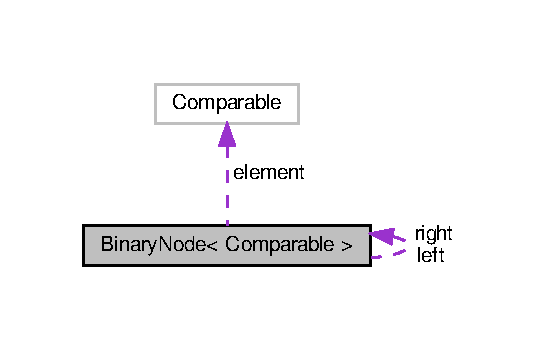
\includegraphics[width=258pt]{classBinaryNode__coll__graph}
\end{center}
\end{figure}
\subsection*{Private Member Functions}
\begin{DoxyCompactItemize}
\item 
\hyperlink{classBinaryNode_aff89d3679c077d70b67ad16e9816d884}{Binary\+Node} (const Comparable \&the\+Element, \hyperlink{classBinaryNode}{Binary\+Node} $\ast$lt, \hyperlink{classBinaryNode}{Binary\+Node} $\ast$rt)
\end{DoxyCompactItemize}
\subsection*{Private Attributes}
\begin{DoxyCompactItemize}
\item 
Comparable \hyperlink{classBinaryNode_a75804c1624577ae485b775408b54bd06}{element}
\item 
\hyperlink{classBinaryNode}{Binary\+Node} $\ast$ \hyperlink{classBinaryNode_a2b6352b5519f90f2d9c2d610b2278dac}{left}
\item 
\hyperlink{classBinaryNode}{Binary\+Node} $\ast$ \hyperlink{classBinaryNode_a847342c242923f34b77fc5e402fbbb4b}{right}
\end{DoxyCompactItemize}
\subsection*{Friends}
\begin{DoxyCompactItemize}
\item 
class \hyperlink{classBinaryNode_a28a1adb9906f3ff7e12c2cb6fa2bd54e}{B\+S\+T$<$ Comparable $>$}
\item 
class \hyperlink{classBinaryNode_aab3993acac2ab24a0b59edb0c3acc775}{B\+S\+T\+Itr\+In$<$ Comparable $>$}
\item 
class \hyperlink{classBinaryNode_a45a55df6f11541416d4ea7684c575c1a}{B\+S\+T\+Itr\+Pre$<$ Comparable $>$}
\item 
class \hyperlink{classBinaryNode_a5dc153694be266f6e772659486219da7}{B\+S\+T\+Itr\+Post$<$ Comparable $>$}
\item 
class \hyperlink{classBinaryNode_a26ff00bc0d87069aed877f10fd3c80a8}{B\+S\+T\+Itr\+Level$<$ Comparable $>$}
\end{DoxyCompactItemize}


\subsection{Constructor \& Destructor Documentation}
\mbox{\Hypertarget{classBinaryNode_aff89d3679c077d70b67ad16e9816d884}\label{classBinaryNode_aff89d3679c077d70b67ad16e9816d884}} 
\index{Binary\+Node@{Binary\+Node}!Binary\+Node@{Binary\+Node}}
\index{Binary\+Node@{Binary\+Node}!Binary\+Node@{Binary\+Node}}
\subsubsection{\texorpdfstring{Binary\+Node()}{BinaryNode()}}
{\footnotesize\ttfamily template$<$class Comparable$>$ \\
\hyperlink{classBinaryNode}{Binary\+Node}$<$ Comparable $>$\+::\hyperlink{classBinaryNode}{Binary\+Node} (\begin{DoxyParamCaption}\item[{const Comparable \&}]{the\+Element,  }\item[{\hyperlink{classBinaryNode}{Binary\+Node}$<$ Comparable $>$ $\ast$}]{lt,  }\item[{\hyperlink{classBinaryNode}{Binary\+Node}$<$ Comparable $>$ $\ast$}]{rt }\end{DoxyParamCaption})\hspace{0.3cm}{\ttfamily [inline]}, {\ttfamily [private]}}



\subsection{Friends And Related Function Documentation}
\mbox{\Hypertarget{classBinaryNode_a28a1adb9906f3ff7e12c2cb6fa2bd54e}\label{classBinaryNode_a28a1adb9906f3ff7e12c2cb6fa2bd54e}} 
\index{Binary\+Node@{Binary\+Node}!B\+S\+T$<$ Comparable $>$@{B\+S\+T$<$ Comparable $>$}}
\index{B\+S\+T$<$ Comparable $>$@{B\+S\+T$<$ Comparable $>$}!Binary\+Node@{Binary\+Node}}
\subsubsection{\texorpdfstring{B\+S\+T$<$ Comparable $>$}{BST< Comparable >}}
{\footnotesize\ttfamily template$<$class Comparable$>$ \\
friend class \hyperlink{classBST}{B\+ST}$<$ Comparable $>$\hspace{0.3cm}{\ttfamily [friend]}}

\mbox{\Hypertarget{classBinaryNode_aab3993acac2ab24a0b59edb0c3acc775}\label{classBinaryNode_aab3993acac2ab24a0b59edb0c3acc775}} 
\index{Binary\+Node@{Binary\+Node}!B\+S\+T\+Itr\+In$<$ Comparable $>$@{B\+S\+T\+Itr\+In$<$ Comparable $>$}}
\index{B\+S\+T\+Itr\+In$<$ Comparable $>$@{B\+S\+T\+Itr\+In$<$ Comparable $>$}!Binary\+Node@{Binary\+Node}}
\subsubsection{\texorpdfstring{B\+S\+T\+Itr\+In$<$ Comparable $>$}{BSTItrIn< Comparable >}}
{\footnotesize\ttfamily template$<$class Comparable$>$ \\
friend class \hyperlink{classBSTItrIn}{B\+S\+T\+Itr\+In}$<$ Comparable $>$\hspace{0.3cm}{\ttfamily [friend]}}

\mbox{\Hypertarget{classBinaryNode_a26ff00bc0d87069aed877f10fd3c80a8}\label{classBinaryNode_a26ff00bc0d87069aed877f10fd3c80a8}} 
\index{Binary\+Node@{Binary\+Node}!B\+S\+T\+Itr\+Level$<$ Comparable $>$@{B\+S\+T\+Itr\+Level$<$ Comparable $>$}}
\index{B\+S\+T\+Itr\+Level$<$ Comparable $>$@{B\+S\+T\+Itr\+Level$<$ Comparable $>$}!Binary\+Node@{Binary\+Node}}
\subsubsection{\texorpdfstring{B\+S\+T\+Itr\+Level$<$ Comparable $>$}{BSTItrLevel< Comparable >}}
{\footnotesize\ttfamily template$<$class Comparable$>$ \\
friend class \hyperlink{classBSTItrLevel}{B\+S\+T\+Itr\+Level}$<$ Comparable $>$\hspace{0.3cm}{\ttfamily [friend]}}

\mbox{\Hypertarget{classBinaryNode_a5dc153694be266f6e772659486219da7}\label{classBinaryNode_a5dc153694be266f6e772659486219da7}} 
\index{Binary\+Node@{Binary\+Node}!B\+S\+T\+Itr\+Post$<$ Comparable $>$@{B\+S\+T\+Itr\+Post$<$ Comparable $>$}}
\index{B\+S\+T\+Itr\+Post$<$ Comparable $>$@{B\+S\+T\+Itr\+Post$<$ Comparable $>$}!Binary\+Node@{Binary\+Node}}
\subsubsection{\texorpdfstring{B\+S\+T\+Itr\+Post$<$ Comparable $>$}{BSTItrPost< Comparable >}}
{\footnotesize\ttfamily template$<$class Comparable$>$ \\
friend class \hyperlink{classBSTItrPost}{B\+S\+T\+Itr\+Post}$<$ Comparable $>$\hspace{0.3cm}{\ttfamily [friend]}}

\mbox{\Hypertarget{classBinaryNode_a45a55df6f11541416d4ea7684c575c1a}\label{classBinaryNode_a45a55df6f11541416d4ea7684c575c1a}} 
\index{Binary\+Node@{Binary\+Node}!B\+S\+T\+Itr\+Pre$<$ Comparable $>$@{B\+S\+T\+Itr\+Pre$<$ Comparable $>$}}
\index{B\+S\+T\+Itr\+Pre$<$ Comparable $>$@{B\+S\+T\+Itr\+Pre$<$ Comparable $>$}!Binary\+Node@{Binary\+Node}}
\subsubsection{\texorpdfstring{B\+S\+T\+Itr\+Pre$<$ Comparable $>$}{BSTItrPre< Comparable >}}
{\footnotesize\ttfamily template$<$class Comparable$>$ \\
friend class \hyperlink{classBSTItrPre}{B\+S\+T\+Itr\+Pre}$<$ Comparable $>$\hspace{0.3cm}{\ttfamily [friend]}}



\subsection{Member Data Documentation}
\mbox{\Hypertarget{classBinaryNode_a75804c1624577ae485b775408b54bd06}\label{classBinaryNode_a75804c1624577ae485b775408b54bd06}} 
\index{Binary\+Node@{Binary\+Node}!element@{element}}
\index{element@{element}!Binary\+Node@{Binary\+Node}}
\subsubsection{\texorpdfstring{element}{element}}
{\footnotesize\ttfamily template$<$class Comparable$>$ \\
Comparable \hyperlink{classBinaryNode}{Binary\+Node}$<$ Comparable $>$\+::element\hspace{0.3cm}{\ttfamily [private]}}

\mbox{\Hypertarget{classBinaryNode_a2b6352b5519f90f2d9c2d610b2278dac}\label{classBinaryNode_a2b6352b5519f90f2d9c2d610b2278dac}} 
\index{Binary\+Node@{Binary\+Node}!left@{left}}
\index{left@{left}!Binary\+Node@{Binary\+Node}}
\subsubsection{\texorpdfstring{left}{left}}
{\footnotesize\ttfamily template$<$class Comparable$>$ \\
\hyperlink{classBinaryNode}{Binary\+Node}$\ast$ \hyperlink{classBinaryNode}{Binary\+Node}$<$ Comparable $>$\+::left\hspace{0.3cm}{\ttfamily [private]}}

\mbox{\Hypertarget{classBinaryNode_a847342c242923f34b77fc5e402fbbb4b}\label{classBinaryNode_a847342c242923f34b77fc5e402fbbb4b}} 
\index{Binary\+Node@{Binary\+Node}!right@{right}}
\index{right@{right}!Binary\+Node@{Binary\+Node}}
\subsubsection{\texorpdfstring{right}{right}}
{\footnotesize\ttfamily template$<$class Comparable$>$ \\
\hyperlink{classBinaryNode}{Binary\+Node}$\ast$ \hyperlink{classBinaryNode}{Binary\+Node}$<$ Comparable $>$\+::right\hspace{0.3cm}{\ttfamily [private]}}



The documentation for this class was generated from the following file\+:\begin{DoxyCompactItemize}
\item 
src/\hyperlink{BST_8h}{B\+S\+T.\+h}\end{DoxyCompactItemize}

\hypertarget{classBST}{}\section{B\+ST$<$ Comparable $>$ Class Template Reference}
\label{classBST}\index{B\+S\+T$<$ Comparable $>$@{B\+S\+T$<$ Comparable $>$}}


{\ttfamily \#include $<$B\+S\+T.\+h$>$}



Collaboration diagram for B\+ST$<$ Comparable $>$\+:\nopagebreak
\begin{figure}[H]
\begin{center}
\leavevmode
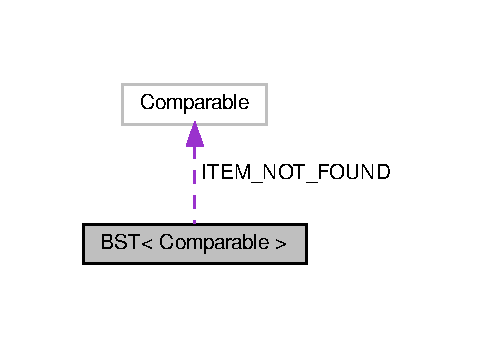
\includegraphics[width=229pt]{classBST__coll__graph}
\end{center}
\end{figure}
\subsection*{Public Member Functions}
\begin{DoxyCompactItemize}
\item 
\hyperlink{classBST_a3185a79cf472271f122a97d0f59022d1}{B\+ST} (const Comparable \&not\+Found)
\item 
\hyperlink{classBST_a163232cc6ffcbd1a51707efcc3fa36ca}{B\+ST} (const \hyperlink{classBST}{B\+ST} \&rhs)
\item 
\hyperlink{classBST_abf3125f968641c8726101c5dd18f36be}{$\sim$\+B\+ST} ()
\item 
const Comparable \& \hyperlink{classBST_aa52491ff35aec517961937a17a9fa493}{find\+Min} () const
\item 
const Comparable \& \hyperlink{classBST_a03485f3b0b150f1e69a12c28d26d8092}{find\+Max} () const
\item 
const Comparable \& \hyperlink{classBST_aaf4eb6869f68db0069534f7b2dfbe53b}{find} (const Comparable \&x) const
\item 
bool \hyperlink{classBST_a10fd737b2be62437023407fdc123f728}{is\+Empty} () const
\item 
void \hyperlink{classBST_a91e830925c48040d4c4dbb7d971c3bfe}{print\+Tree} () const
\item 
void \hyperlink{classBST_a050d829503a88714c4ad0773cf6d3af6}{make\+Empty} ()
\item 
void \hyperlink{classBST_a2b117df6521c7d61dac75ff2c938bae7}{insert} (const Comparable \&x)
\item 
void \hyperlink{classBST_a6f01a0b44daf82a42022b6eb4c0df7a2}{remove} (const Comparable \&x)
\item 
const \hyperlink{classBST}{B\+ST} \& \hyperlink{classBST_aa80c39f454c89d4a202be3d1445823f3}{operator=} (const \hyperlink{classBST}{B\+ST} \&rhs)
\end{DoxyCompactItemize}
\subsection*{Private Member Functions}
\begin{DoxyCompactItemize}
\item 
const Comparable \& \hyperlink{classBST_adb7d0e1197c30ff79cb0fb05fcd67249}{element\+At} (\hyperlink{classBinaryNode}{Binary\+Node}$<$ Comparable $>$ $\ast$t) const
\item 
void \hyperlink{classBST_a4d885d655c4a4e29c2d40f2b48baf7d3}{insert} (const Comparable \&x, \hyperlink{classBinaryNode}{Binary\+Node}$<$ Comparable $>$ $\ast$\&t) const
\item 
void \hyperlink{classBST_afe360f55921ac51ac78ddde6556fe946}{remove} (const Comparable \&x, \hyperlink{classBinaryNode}{Binary\+Node}$<$ Comparable $>$ $\ast$\&t) const
\item 
\hyperlink{classBinaryNode}{Binary\+Node}$<$ Comparable $>$ $\ast$ \hyperlink{classBST_a1b79bb91ccef69398a80bf508a2a6097}{find\+Min} (\hyperlink{classBinaryNode}{Binary\+Node}$<$ Comparable $>$ $\ast$t) const
\item 
\hyperlink{classBinaryNode}{Binary\+Node}$<$ Comparable $>$ $\ast$ \hyperlink{classBST_a922e4c2dfbd460db9e31531d8d20282b}{find\+Max} (\hyperlink{classBinaryNode}{Binary\+Node}$<$ Comparable $>$ $\ast$t) const
\item 
\hyperlink{classBinaryNode}{Binary\+Node}$<$ Comparable $>$ $\ast$ \hyperlink{classBST_a858dd15e9d15affeb88785d0c5a65ae3}{find} (const Comparable \&x, \hyperlink{classBinaryNode}{Binary\+Node}$<$ Comparable $>$ $\ast$t) const
\item 
void \hyperlink{classBST_a5582f1066a084181d6a79ec0a6e9f9f2}{make\+Empty} (\hyperlink{classBinaryNode}{Binary\+Node}$<$ Comparable $>$ $\ast$\&t) const
\item 
void \hyperlink{classBST_a76247d69325065d2485349148d7940e7}{print\+Tree} (\hyperlink{classBinaryNode}{Binary\+Node}$<$ Comparable $>$ $\ast$t) const
\item 
\hyperlink{classBinaryNode}{Binary\+Node}$<$ Comparable $>$ $\ast$ \hyperlink{classBST_acefda5ede0b55cbb1f7deab580bd8fd9}{clone} (\hyperlink{classBinaryNode}{Binary\+Node}$<$ Comparable $>$ $\ast$t) const
\end{DoxyCompactItemize}
\subsection*{Private Attributes}
\begin{DoxyCompactItemize}
\item 
\hyperlink{classBinaryNode}{Binary\+Node}$<$ Comparable $>$ $\ast$ \hyperlink{classBST_a48d08a19c48c0c260a7d5db37149ad0f}{root}
\item 
const Comparable \hyperlink{classBST_a93811f042c4201e993fe39638c15f251}{I\+T\+E\+M\+\_\+\+N\+O\+T\+\_\+\+F\+O\+U\+ND}
\end{DoxyCompactItemize}
\subsection*{Friends}
\begin{DoxyCompactItemize}
\item 
class \hyperlink{classBST_aab3993acac2ab24a0b59edb0c3acc775}{B\+S\+T\+Itr\+In$<$ Comparable $>$}
\item 
class \hyperlink{classBST_a45a55df6f11541416d4ea7684c575c1a}{B\+S\+T\+Itr\+Pre$<$ Comparable $>$}
\item 
class \hyperlink{classBST_a5dc153694be266f6e772659486219da7}{B\+S\+T\+Itr\+Post$<$ Comparable $>$}
\item 
class \hyperlink{classBST_a26ff00bc0d87069aed877f10fd3c80a8}{B\+S\+T\+Itr\+Level$<$ Comparable $>$}
\end{DoxyCompactItemize}


\subsection{Constructor \& Destructor Documentation}
\mbox{\Hypertarget{classBST_a3185a79cf472271f122a97d0f59022d1}\label{classBST_a3185a79cf472271f122a97d0f59022d1}} 
\index{B\+ST@{B\+ST}!B\+ST@{B\+ST}}
\index{B\+ST@{B\+ST}!B\+ST@{B\+ST}}
\subsubsection{\texorpdfstring{B\+S\+T()}{BST()}\hspace{0.1cm}{\footnotesize\ttfamily [1/2]}}
{\footnotesize\ttfamily template$<$class Comparable$>$ \\
\hyperlink{classBST}{B\+ST}$<$ Comparable $>$\+::\hyperlink{classBST}{B\+ST} (\begin{DoxyParamCaption}\item[{const Comparable \&}]{not\+Found }\end{DoxyParamCaption})\hspace{0.3cm}{\ttfamily [explicit]}}

\mbox{\Hypertarget{classBST_a163232cc6ffcbd1a51707efcc3fa36ca}\label{classBST_a163232cc6ffcbd1a51707efcc3fa36ca}} 
\index{B\+ST@{B\+ST}!B\+ST@{B\+ST}}
\index{B\+ST@{B\+ST}!B\+ST@{B\+ST}}
\subsubsection{\texorpdfstring{B\+S\+T()}{BST()}\hspace{0.1cm}{\footnotesize\ttfamily [2/2]}}
{\footnotesize\ttfamily template$<$class Comparable$>$ \\
\hyperlink{classBST}{B\+ST}$<$ Comparable $>$\+::\hyperlink{classBST}{B\+ST} (\begin{DoxyParamCaption}\item[{const \hyperlink{classBST}{B\+ST}$<$ Comparable $>$ \&}]{rhs }\end{DoxyParamCaption})}

\mbox{\Hypertarget{classBST_abf3125f968641c8726101c5dd18f36be}\label{classBST_abf3125f968641c8726101c5dd18f36be}} 
\index{B\+ST@{B\+ST}!````~B\+ST@{$\sim$\+B\+ST}}
\index{````~B\+ST@{$\sim$\+B\+ST}!B\+ST@{B\+ST}}
\subsubsection{\texorpdfstring{$\sim$\+B\+S\+T()}{~BST()}}
{\footnotesize\ttfamily template$<$class Comparable $>$ \\
\hyperlink{classBST}{B\+ST}$<$ Comparable $>$\+::$\sim$\hyperlink{classBST}{B\+ST} (\begin{DoxyParamCaption}{ }\end{DoxyParamCaption})}



\subsection{Member Function Documentation}
\mbox{\Hypertarget{classBST_acefda5ede0b55cbb1f7deab580bd8fd9}\label{classBST_acefda5ede0b55cbb1f7deab580bd8fd9}} 
\index{B\+ST@{B\+ST}!clone@{clone}}
\index{clone@{clone}!B\+ST@{B\+ST}}
\subsubsection{\texorpdfstring{clone()}{clone()}}
{\footnotesize\ttfamily template$<$class Comparable$>$ \\
\hyperlink{classBinaryNode}{Binary\+Node}$<$ Comparable $>$ $\ast$ \hyperlink{classBST}{B\+ST}$<$ Comparable $>$\+::clone (\begin{DoxyParamCaption}\item[{\hyperlink{classBinaryNode}{Binary\+Node}$<$ Comparable $>$ $\ast$}]{t }\end{DoxyParamCaption}) const\hspace{0.3cm}{\ttfamily [private]}}

\mbox{\Hypertarget{classBST_adb7d0e1197c30ff79cb0fb05fcd67249}\label{classBST_adb7d0e1197c30ff79cb0fb05fcd67249}} 
\index{B\+ST@{B\+ST}!element\+At@{element\+At}}
\index{element\+At@{element\+At}!B\+ST@{B\+ST}}
\subsubsection{\texorpdfstring{element\+At()}{elementAt()}}
{\footnotesize\ttfamily template$<$class Comparable$>$ \\
const Comparable \& \hyperlink{classBST}{B\+ST}$<$ Comparable $>$\+::element\+At (\begin{DoxyParamCaption}\item[{\hyperlink{classBinaryNode}{Binary\+Node}$<$ Comparable $>$ $\ast$}]{t }\end{DoxyParamCaption}) const\hspace{0.3cm}{\ttfamily [private]}}

\mbox{\Hypertarget{classBST_aaf4eb6869f68db0069534f7b2dfbe53b}\label{classBST_aaf4eb6869f68db0069534f7b2dfbe53b}} 
\index{B\+ST@{B\+ST}!find@{find}}
\index{find@{find}!B\+ST@{B\+ST}}
\subsubsection{\texorpdfstring{find()}{find()}\hspace{0.1cm}{\footnotesize\ttfamily [1/2]}}
{\footnotesize\ttfamily template$<$class Comparable$>$ \\
const Comparable \& \hyperlink{classBST}{B\+ST}$<$ Comparable $>$\+::find (\begin{DoxyParamCaption}\item[{const Comparable \&}]{x }\end{DoxyParamCaption}) const}

\mbox{\Hypertarget{classBST_a858dd15e9d15affeb88785d0c5a65ae3}\label{classBST_a858dd15e9d15affeb88785d0c5a65ae3}} 
\index{B\+ST@{B\+ST}!find@{find}}
\index{find@{find}!B\+ST@{B\+ST}}
\subsubsection{\texorpdfstring{find()}{find()}\hspace{0.1cm}{\footnotesize\ttfamily [2/2]}}
{\footnotesize\ttfamily template$<$class Comparable$>$ \\
\hyperlink{classBinaryNode}{Binary\+Node}$<$ Comparable $>$ $\ast$ \hyperlink{classBST}{B\+ST}$<$ Comparable $>$\+::find (\begin{DoxyParamCaption}\item[{const Comparable \&}]{x,  }\item[{\hyperlink{classBinaryNode}{Binary\+Node}$<$ Comparable $>$ $\ast$}]{t }\end{DoxyParamCaption}) const\hspace{0.3cm}{\ttfamily [private]}}

\mbox{\Hypertarget{classBST_a03485f3b0b150f1e69a12c28d26d8092}\label{classBST_a03485f3b0b150f1e69a12c28d26d8092}} 
\index{B\+ST@{B\+ST}!find\+Max@{find\+Max}}
\index{find\+Max@{find\+Max}!B\+ST@{B\+ST}}
\subsubsection{\texorpdfstring{find\+Max()}{findMax()}\hspace{0.1cm}{\footnotesize\ttfamily [1/2]}}
{\footnotesize\ttfamily template$<$class Comparable $>$ \\
const Comparable \& \hyperlink{classBST}{B\+ST}$<$ Comparable $>$\+::find\+Max (\begin{DoxyParamCaption}{ }\end{DoxyParamCaption}) const}

\mbox{\Hypertarget{classBST_a922e4c2dfbd460db9e31531d8d20282b}\label{classBST_a922e4c2dfbd460db9e31531d8d20282b}} 
\index{B\+ST@{B\+ST}!find\+Max@{find\+Max}}
\index{find\+Max@{find\+Max}!B\+ST@{B\+ST}}
\subsubsection{\texorpdfstring{find\+Max()}{findMax()}\hspace{0.1cm}{\footnotesize\ttfamily [2/2]}}
{\footnotesize\ttfamily template$<$class Comparable$>$ \\
\hyperlink{classBinaryNode}{Binary\+Node}$<$ Comparable $>$ $\ast$ \hyperlink{classBST}{B\+ST}$<$ Comparable $>$\+::find\+Max (\begin{DoxyParamCaption}\item[{\hyperlink{classBinaryNode}{Binary\+Node}$<$ Comparable $>$ $\ast$}]{t }\end{DoxyParamCaption}) const\hspace{0.3cm}{\ttfamily [private]}}

\mbox{\Hypertarget{classBST_aa52491ff35aec517961937a17a9fa493}\label{classBST_aa52491ff35aec517961937a17a9fa493}} 
\index{B\+ST@{B\+ST}!find\+Min@{find\+Min}}
\index{find\+Min@{find\+Min}!B\+ST@{B\+ST}}
\subsubsection{\texorpdfstring{find\+Min()}{findMin()}\hspace{0.1cm}{\footnotesize\ttfamily [1/2]}}
{\footnotesize\ttfamily template$<$class Comparable $>$ \\
const Comparable \& \hyperlink{classBST}{B\+ST}$<$ Comparable $>$\+::find\+Min (\begin{DoxyParamCaption}{ }\end{DoxyParamCaption}) const}

\mbox{\Hypertarget{classBST_a1b79bb91ccef69398a80bf508a2a6097}\label{classBST_a1b79bb91ccef69398a80bf508a2a6097}} 
\index{B\+ST@{B\+ST}!find\+Min@{find\+Min}}
\index{find\+Min@{find\+Min}!B\+ST@{B\+ST}}
\subsubsection{\texorpdfstring{find\+Min()}{findMin()}\hspace{0.1cm}{\footnotesize\ttfamily [2/2]}}
{\footnotesize\ttfamily template$<$class Comparable$>$ \\
\hyperlink{classBinaryNode}{Binary\+Node}$<$ Comparable $>$ $\ast$ \hyperlink{classBST}{B\+ST}$<$ Comparable $>$\+::find\+Min (\begin{DoxyParamCaption}\item[{\hyperlink{classBinaryNode}{Binary\+Node}$<$ Comparable $>$ $\ast$}]{t }\end{DoxyParamCaption}) const\hspace{0.3cm}{\ttfamily [private]}}

\mbox{\Hypertarget{classBST_a2b117df6521c7d61dac75ff2c938bae7}\label{classBST_a2b117df6521c7d61dac75ff2c938bae7}} 
\index{B\+ST@{B\+ST}!insert@{insert}}
\index{insert@{insert}!B\+ST@{B\+ST}}
\subsubsection{\texorpdfstring{insert()}{insert()}\hspace{0.1cm}{\footnotesize\ttfamily [1/2]}}
{\footnotesize\ttfamily template$<$class Comparable$>$ \\
void \hyperlink{classBST}{B\+ST}$<$ Comparable $>$\+::insert (\begin{DoxyParamCaption}\item[{const Comparable \&}]{x }\end{DoxyParamCaption})}

\mbox{\Hypertarget{classBST_a4d885d655c4a4e29c2d40f2b48baf7d3}\label{classBST_a4d885d655c4a4e29c2d40f2b48baf7d3}} 
\index{B\+ST@{B\+ST}!insert@{insert}}
\index{insert@{insert}!B\+ST@{B\+ST}}
\subsubsection{\texorpdfstring{insert()}{insert()}\hspace{0.1cm}{\footnotesize\ttfamily [2/2]}}
{\footnotesize\ttfamily template$<$class Comparable$>$ \\
void \hyperlink{classBST}{B\+ST}$<$ Comparable $>$\+::insert (\begin{DoxyParamCaption}\item[{const Comparable \&}]{x,  }\item[{\hyperlink{classBinaryNode}{Binary\+Node}$<$ Comparable $>$ $\ast$\&}]{t }\end{DoxyParamCaption}) const\hspace{0.3cm}{\ttfamily [private]}}

\mbox{\Hypertarget{classBST_a10fd737b2be62437023407fdc123f728}\label{classBST_a10fd737b2be62437023407fdc123f728}} 
\index{B\+ST@{B\+ST}!is\+Empty@{is\+Empty}}
\index{is\+Empty@{is\+Empty}!B\+ST@{B\+ST}}
\subsubsection{\texorpdfstring{is\+Empty()}{isEmpty()}}
{\footnotesize\ttfamily template$<$class Comparable $>$ \\
bool \hyperlink{classBST}{B\+ST}$<$ Comparable $>$\+::is\+Empty (\begin{DoxyParamCaption}{ }\end{DoxyParamCaption}) const}

\mbox{\Hypertarget{classBST_a050d829503a88714c4ad0773cf6d3af6}\label{classBST_a050d829503a88714c4ad0773cf6d3af6}} 
\index{B\+ST@{B\+ST}!make\+Empty@{make\+Empty}}
\index{make\+Empty@{make\+Empty}!B\+ST@{B\+ST}}
\subsubsection{\texorpdfstring{make\+Empty()}{makeEmpty()}\hspace{0.1cm}{\footnotesize\ttfamily [1/2]}}
{\footnotesize\ttfamily template$<$class Comparable $>$ \\
void \hyperlink{classBST}{B\+ST}$<$ Comparable $>$\+::make\+Empty (\begin{DoxyParamCaption}{ }\end{DoxyParamCaption})}

\mbox{\Hypertarget{classBST_a5582f1066a084181d6a79ec0a6e9f9f2}\label{classBST_a5582f1066a084181d6a79ec0a6e9f9f2}} 
\index{B\+ST@{B\+ST}!make\+Empty@{make\+Empty}}
\index{make\+Empty@{make\+Empty}!B\+ST@{B\+ST}}
\subsubsection{\texorpdfstring{make\+Empty()}{makeEmpty()}\hspace{0.1cm}{\footnotesize\ttfamily [2/2]}}
{\footnotesize\ttfamily template$<$class Comparable$>$ \\
void \hyperlink{classBST}{B\+ST}$<$ Comparable $>$\+::make\+Empty (\begin{DoxyParamCaption}\item[{\hyperlink{classBinaryNode}{Binary\+Node}$<$ Comparable $>$ $\ast$\&}]{t }\end{DoxyParamCaption}) const\hspace{0.3cm}{\ttfamily [private]}}

Internal method to make subtree empty. \mbox{\Hypertarget{classBST_aa80c39f454c89d4a202be3d1445823f3}\label{classBST_aa80c39f454c89d4a202be3d1445823f3}} 
\index{B\+ST@{B\+ST}!operator=@{operator=}}
\index{operator=@{operator=}!B\+ST@{B\+ST}}
\subsubsection{\texorpdfstring{operator=()}{operator=()}}
{\footnotesize\ttfamily template$<$class Comparable $>$ \\
const \hyperlink{classBST}{B\+ST}$<$ Comparable $>$ \& \hyperlink{classBST}{B\+ST}$<$ Comparable $>$\+::operator= (\begin{DoxyParamCaption}\item[{const \hyperlink{classBST}{B\+ST}$<$ Comparable $>$ \&}]{rhs }\end{DoxyParamCaption})}

\mbox{\Hypertarget{classBST_a91e830925c48040d4c4dbb7d971c3bfe}\label{classBST_a91e830925c48040d4c4dbb7d971c3bfe}} 
\index{B\+ST@{B\+ST}!print\+Tree@{print\+Tree}}
\index{print\+Tree@{print\+Tree}!B\+ST@{B\+ST}}
\subsubsection{\texorpdfstring{print\+Tree()}{printTree()}\hspace{0.1cm}{\footnotesize\ttfamily [1/2]}}
{\footnotesize\ttfamily template$<$class Comparable $>$ \\
void \hyperlink{classBST}{B\+ST}$<$ Comparable $>$\+::print\+Tree (\begin{DoxyParamCaption}{ }\end{DoxyParamCaption}) const}

\mbox{\Hypertarget{classBST_a76247d69325065d2485349148d7940e7}\label{classBST_a76247d69325065d2485349148d7940e7}} 
\index{B\+ST@{B\+ST}!print\+Tree@{print\+Tree}}
\index{print\+Tree@{print\+Tree}!B\+ST@{B\+ST}}
\subsubsection{\texorpdfstring{print\+Tree()}{printTree()}\hspace{0.1cm}{\footnotesize\ttfamily [2/2]}}
{\footnotesize\ttfamily template$<$class Comparable$>$ \\
void \hyperlink{classBST}{B\+ST}$<$ Comparable $>$\+::print\+Tree (\begin{DoxyParamCaption}\item[{\hyperlink{classBinaryNode}{Binary\+Node}$<$ Comparable $>$ $\ast$}]{t }\end{DoxyParamCaption}) const\hspace{0.3cm}{\ttfamily [private]}}

\mbox{\Hypertarget{classBST_a6f01a0b44daf82a42022b6eb4c0df7a2}\label{classBST_a6f01a0b44daf82a42022b6eb4c0df7a2}} 
\index{B\+ST@{B\+ST}!remove@{remove}}
\index{remove@{remove}!B\+ST@{B\+ST}}
\subsubsection{\texorpdfstring{remove()}{remove()}\hspace{0.1cm}{\footnotesize\ttfamily [1/2]}}
{\footnotesize\ttfamily template$<$class Comparable$>$ \\
void \hyperlink{classBST}{B\+ST}$<$ Comparable $>$\+::remove (\begin{DoxyParamCaption}\item[{const Comparable \&}]{x }\end{DoxyParamCaption})}

\mbox{\Hypertarget{classBST_afe360f55921ac51ac78ddde6556fe946}\label{classBST_afe360f55921ac51ac78ddde6556fe946}} 
\index{B\+ST@{B\+ST}!remove@{remove}}
\index{remove@{remove}!B\+ST@{B\+ST}}
\subsubsection{\texorpdfstring{remove()}{remove()}\hspace{0.1cm}{\footnotesize\ttfamily [2/2]}}
{\footnotesize\ttfamily template$<$class Comparable$>$ \\
void \hyperlink{classBST}{B\+ST}$<$ Comparable $>$\+::remove (\begin{DoxyParamCaption}\item[{const Comparable \&}]{x,  }\item[{\hyperlink{classBinaryNode}{Binary\+Node}$<$ Comparable $>$ $\ast$\&}]{t }\end{DoxyParamCaption}) const\hspace{0.3cm}{\ttfamily [private]}}



\subsection{Friends And Related Function Documentation}
\mbox{\Hypertarget{classBST_aab3993acac2ab24a0b59edb0c3acc775}\label{classBST_aab3993acac2ab24a0b59edb0c3acc775}} 
\index{B\+ST@{B\+ST}!B\+S\+T\+Itr\+In$<$ Comparable $>$@{B\+S\+T\+Itr\+In$<$ Comparable $>$}}
\index{B\+S\+T\+Itr\+In$<$ Comparable $>$@{B\+S\+T\+Itr\+In$<$ Comparable $>$}!B\+ST@{B\+ST}}
\subsubsection{\texorpdfstring{B\+S\+T\+Itr\+In$<$ Comparable $>$}{BSTItrIn< Comparable >}}
{\footnotesize\ttfamily template$<$class Comparable$>$ \\
friend class \hyperlink{classBSTItrIn}{B\+S\+T\+Itr\+In}$<$ Comparable $>$\hspace{0.3cm}{\ttfamily [friend]}}

\mbox{\Hypertarget{classBST_a26ff00bc0d87069aed877f10fd3c80a8}\label{classBST_a26ff00bc0d87069aed877f10fd3c80a8}} 
\index{B\+ST@{B\+ST}!B\+S\+T\+Itr\+Level$<$ Comparable $>$@{B\+S\+T\+Itr\+Level$<$ Comparable $>$}}
\index{B\+S\+T\+Itr\+Level$<$ Comparable $>$@{B\+S\+T\+Itr\+Level$<$ Comparable $>$}!B\+ST@{B\+ST}}
\subsubsection{\texorpdfstring{B\+S\+T\+Itr\+Level$<$ Comparable $>$}{BSTItrLevel< Comparable >}}
{\footnotesize\ttfamily template$<$class Comparable$>$ \\
friend class \hyperlink{classBSTItrLevel}{B\+S\+T\+Itr\+Level}$<$ Comparable $>$\hspace{0.3cm}{\ttfamily [friend]}}

\mbox{\Hypertarget{classBST_a5dc153694be266f6e772659486219da7}\label{classBST_a5dc153694be266f6e772659486219da7}} 
\index{B\+ST@{B\+ST}!B\+S\+T\+Itr\+Post$<$ Comparable $>$@{B\+S\+T\+Itr\+Post$<$ Comparable $>$}}
\index{B\+S\+T\+Itr\+Post$<$ Comparable $>$@{B\+S\+T\+Itr\+Post$<$ Comparable $>$}!B\+ST@{B\+ST}}
\subsubsection{\texorpdfstring{B\+S\+T\+Itr\+Post$<$ Comparable $>$}{BSTItrPost< Comparable >}}
{\footnotesize\ttfamily template$<$class Comparable$>$ \\
friend class \hyperlink{classBSTItrPost}{B\+S\+T\+Itr\+Post}$<$ Comparable $>$\hspace{0.3cm}{\ttfamily [friend]}}

\mbox{\Hypertarget{classBST_a45a55df6f11541416d4ea7684c575c1a}\label{classBST_a45a55df6f11541416d4ea7684c575c1a}} 
\index{B\+ST@{B\+ST}!B\+S\+T\+Itr\+Pre$<$ Comparable $>$@{B\+S\+T\+Itr\+Pre$<$ Comparable $>$}}
\index{B\+S\+T\+Itr\+Pre$<$ Comparable $>$@{B\+S\+T\+Itr\+Pre$<$ Comparable $>$}!B\+ST@{B\+ST}}
\subsubsection{\texorpdfstring{B\+S\+T\+Itr\+Pre$<$ Comparable $>$}{BSTItrPre< Comparable >}}
{\footnotesize\ttfamily template$<$class Comparable$>$ \\
friend class \hyperlink{classBSTItrPre}{B\+S\+T\+Itr\+Pre}$<$ Comparable $>$\hspace{0.3cm}{\ttfamily [friend]}}



\subsection{Member Data Documentation}
\mbox{\Hypertarget{classBST_a93811f042c4201e993fe39638c15f251}\label{classBST_a93811f042c4201e993fe39638c15f251}} 
\index{B\+ST@{B\+ST}!I\+T\+E\+M\+\_\+\+N\+O\+T\+\_\+\+F\+O\+U\+ND@{I\+T\+E\+M\+\_\+\+N\+O\+T\+\_\+\+F\+O\+U\+ND}}
\index{I\+T\+E\+M\+\_\+\+N\+O\+T\+\_\+\+F\+O\+U\+ND@{I\+T\+E\+M\+\_\+\+N\+O\+T\+\_\+\+F\+O\+U\+ND}!B\+ST@{B\+ST}}
\subsubsection{\texorpdfstring{I\+T\+E\+M\+\_\+\+N\+O\+T\+\_\+\+F\+O\+U\+ND}{ITEM\_NOT\_FOUND}}
{\footnotesize\ttfamily template$<$class Comparable$>$ \\
const Comparable \hyperlink{classBST}{B\+ST}$<$ Comparable $>$\+::I\+T\+E\+M\+\_\+\+N\+O\+T\+\_\+\+F\+O\+U\+ND\hspace{0.3cm}{\ttfamily [private]}}

\mbox{\Hypertarget{classBST_a48d08a19c48c0c260a7d5db37149ad0f}\label{classBST_a48d08a19c48c0c260a7d5db37149ad0f}} 
\index{B\+ST@{B\+ST}!root@{root}}
\index{root@{root}!B\+ST@{B\+ST}}
\subsubsection{\texorpdfstring{root}{root}}
{\footnotesize\ttfamily template$<$class Comparable$>$ \\
\hyperlink{classBinaryNode}{Binary\+Node}$<$Comparable$>$$\ast$ \hyperlink{classBST}{B\+ST}$<$ Comparable $>$\+::root\hspace{0.3cm}{\ttfamily [private]}}



The documentation for this class was generated from the following file\+:\begin{DoxyCompactItemize}
\item 
src/\hyperlink{BST_8h}{B\+S\+T.\+h}\end{DoxyCompactItemize}

\hypertarget{classBSTItrIn}{}\section{B\+S\+T\+Itr\+In$<$ Comparable $>$ Class Template Reference}
\label{classBSTItrIn}\index{B\+S\+T\+Itr\+In$<$ Comparable $>$@{B\+S\+T\+Itr\+In$<$ Comparable $>$}}


{\ttfamily \#include $<$B\+S\+T.\+h$>$}

\subsection*{Public Member Functions}
\begin{DoxyCompactItemize}
\item 
\hyperlink{classBSTItrIn_ac836e2f560fed9cc7ef8e5431a2836cc}{B\+S\+T\+Itr\+In} (const \hyperlink{classBST}{B\+ST}$<$ Comparable $>$ \&bt)
\item 
void \hyperlink{classBSTItrIn_ac772d3ebbac748c5f8cf9bc659f2e32c}{advance} ()
\item 
const Comparable \& \hyperlink{classBSTItrIn_a434375a2d263bf132ab3c4ac878af8ef}{retrieve} ()
\item 
bool \hyperlink{classBSTItrIn_a6f9a43217862c263a9bf15b9a08b889a}{is\+At\+End} ()
\end{DoxyCompactItemize}
\subsection*{Private Member Functions}
\begin{DoxyCompactItemize}
\item 
void \hyperlink{classBSTItrIn_a896191c02da37364153df2363ff28e7e}{slide\+Left} (\hyperlink{classBinaryNode}{Binary\+Node}$<$ Comparable $>$ $\ast$n)
\end{DoxyCompactItemize}
\subsection*{Private Attributes}
\begin{DoxyCompactItemize}
\item 
stack$<$ \hyperlink{classBinaryNode}{Binary\+Node}$<$ Comparable $>$ $\ast$ $>$ \hyperlink{classBSTItrIn_ad7cb5e89f04cf08f5615aa53614dd916}{itr\+Stack}
\end{DoxyCompactItemize}


\subsection{Constructor \& Destructor Documentation}
\mbox{\Hypertarget{classBSTItrIn_ac836e2f560fed9cc7ef8e5431a2836cc}\label{classBSTItrIn_ac836e2f560fed9cc7ef8e5431a2836cc}} 
\index{B\+S\+T\+Itr\+In@{B\+S\+T\+Itr\+In}!B\+S\+T\+Itr\+In@{B\+S\+T\+Itr\+In}}
\index{B\+S\+T\+Itr\+In@{B\+S\+T\+Itr\+In}!B\+S\+T\+Itr\+In@{B\+S\+T\+Itr\+In}}
\subsubsection{\texorpdfstring{B\+S\+T\+Itr\+In()}{BSTItrIn()}}
{\footnotesize\ttfamily template$<$class Comparable $>$ \\
\hyperlink{classBSTItrIn}{B\+S\+T\+Itr\+In}$<$ Comparable $>$\+::\hyperlink{classBSTItrIn}{B\+S\+T\+Itr\+In} (\begin{DoxyParamCaption}\item[{const \hyperlink{classBST}{B\+ST}$<$ Comparable $>$ \&}]{bt }\end{DoxyParamCaption})}

Here is the call graph for this function\+:\nopagebreak
\begin{figure}[H]
\begin{center}
\leavevmode
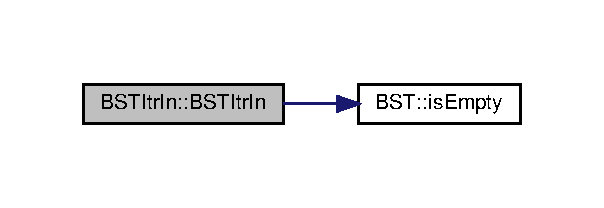
\includegraphics[width=290pt]{classBSTItrIn_ac836e2f560fed9cc7ef8e5431a2836cc_cgraph}
\end{center}
\end{figure}


\subsection{Member Function Documentation}
\mbox{\Hypertarget{classBSTItrIn_ac772d3ebbac748c5f8cf9bc659f2e32c}\label{classBSTItrIn_ac772d3ebbac748c5f8cf9bc659f2e32c}} 
\index{B\+S\+T\+Itr\+In@{B\+S\+T\+Itr\+In}!advance@{advance}}
\index{advance@{advance}!B\+S\+T\+Itr\+In@{B\+S\+T\+Itr\+In}}
\subsubsection{\texorpdfstring{advance()}{advance()}}
{\footnotesize\ttfamily template$<$class Comparable $>$ \\
void \hyperlink{classBSTItrIn}{B\+S\+T\+Itr\+In}$<$ Comparable $>$\+::advance (\begin{DoxyParamCaption}{ }\end{DoxyParamCaption})}

\mbox{\Hypertarget{classBSTItrIn_a6f9a43217862c263a9bf15b9a08b889a}\label{classBSTItrIn_a6f9a43217862c263a9bf15b9a08b889a}} 
\index{B\+S\+T\+Itr\+In@{B\+S\+T\+Itr\+In}!is\+At\+End@{is\+At\+End}}
\index{is\+At\+End@{is\+At\+End}!B\+S\+T\+Itr\+In@{B\+S\+T\+Itr\+In}}
\subsubsection{\texorpdfstring{is\+At\+End()}{isAtEnd()}}
{\footnotesize\ttfamily template$<$class Comparable$>$ \\
bool \hyperlink{classBSTItrIn}{B\+S\+T\+Itr\+In}$<$ Comparable $>$\+::is\+At\+End (\begin{DoxyParamCaption}{ }\end{DoxyParamCaption})\hspace{0.3cm}{\ttfamily [inline]}}

\mbox{\Hypertarget{classBSTItrIn_a434375a2d263bf132ab3c4ac878af8ef}\label{classBSTItrIn_a434375a2d263bf132ab3c4ac878af8ef}} 
\index{B\+S\+T\+Itr\+In@{B\+S\+T\+Itr\+In}!retrieve@{retrieve}}
\index{retrieve@{retrieve}!B\+S\+T\+Itr\+In@{B\+S\+T\+Itr\+In}}
\subsubsection{\texorpdfstring{retrieve()}{retrieve()}}
{\footnotesize\ttfamily template$<$class Comparable$>$ \\
const Comparable\& \hyperlink{classBSTItrIn}{B\+S\+T\+Itr\+In}$<$ Comparable $>$\+::retrieve (\begin{DoxyParamCaption}{ }\end{DoxyParamCaption})\hspace{0.3cm}{\ttfamily [inline]}}

\mbox{\Hypertarget{classBSTItrIn_a896191c02da37364153df2363ff28e7e}\label{classBSTItrIn_a896191c02da37364153df2363ff28e7e}} 
\index{B\+S\+T\+Itr\+In@{B\+S\+T\+Itr\+In}!slide\+Left@{slide\+Left}}
\index{slide\+Left@{slide\+Left}!B\+S\+T\+Itr\+In@{B\+S\+T\+Itr\+In}}
\subsubsection{\texorpdfstring{slide\+Left()}{slideLeft()}}
{\footnotesize\ttfamily template$<$class Comparable $>$ \\
void \hyperlink{classBSTItrIn}{B\+S\+T\+Itr\+In}$<$ Comparable $>$\+::slide\+Left (\begin{DoxyParamCaption}\item[{\hyperlink{classBinaryNode}{Binary\+Node}$<$ Comparable $>$ $\ast$}]{n }\end{DoxyParamCaption})\hspace{0.3cm}{\ttfamily [private]}}



\subsection{Member Data Documentation}
\mbox{\Hypertarget{classBSTItrIn_ad7cb5e89f04cf08f5615aa53614dd916}\label{classBSTItrIn_ad7cb5e89f04cf08f5615aa53614dd916}} 
\index{B\+S\+T\+Itr\+In@{B\+S\+T\+Itr\+In}!itr\+Stack@{itr\+Stack}}
\index{itr\+Stack@{itr\+Stack}!B\+S\+T\+Itr\+In@{B\+S\+T\+Itr\+In}}
\subsubsection{\texorpdfstring{itr\+Stack}{itrStack}}
{\footnotesize\ttfamily template$<$class Comparable$>$ \\
stack$<$\hyperlink{classBinaryNode}{Binary\+Node}$<$Comparable$>$ $\ast$$>$ \hyperlink{classBSTItrIn}{B\+S\+T\+Itr\+In}$<$ Comparable $>$\+::itr\+Stack\hspace{0.3cm}{\ttfamily [private]}}



The documentation for this class was generated from the following file\+:\begin{DoxyCompactItemize}
\item 
src/\hyperlink{BST_8h}{B\+S\+T.\+h}\end{DoxyCompactItemize}

\hypertarget{classBSTItrLevel}{}\section{B\+S\+T\+Itr\+Level$<$ Comparable $>$ Class Template Reference}
\label{classBSTItrLevel}\index{B\+S\+T\+Itr\+Level$<$ Comparable $>$@{B\+S\+T\+Itr\+Level$<$ Comparable $>$}}


{\ttfamily \#include $<$B\+S\+T.\+h$>$}

\subsection*{Public Member Functions}
\begin{DoxyCompactItemize}
\item 
\hyperlink{classBSTItrLevel_a8fd5cdde93eb182c4cd5cf6b2c5efaeb}{B\+S\+T\+Itr\+Level} (const \hyperlink{classBST}{B\+ST}$<$ Comparable $>$ \&bt)
\item 
void \hyperlink{classBSTItrLevel_ad54a6fa289a59d6050b507abe40d463b}{advance} ()
\item 
const Comparable \& \hyperlink{classBSTItrLevel_a7932a172129cc6ca14b6efeee1b4dd87}{retrieve} ()
\item 
bool \hyperlink{classBSTItrLevel_a89bc8e81dde255fd6bad917cacc0d489}{is\+At\+End} ()
\end{DoxyCompactItemize}
\subsection*{Private Attributes}
\begin{DoxyCompactItemize}
\item 
queue$<$ \hyperlink{classBinaryNode}{Binary\+Node}$<$ Comparable $>$ $\ast$ $>$ \hyperlink{classBSTItrLevel_a6de8f9f3e129e2a358b00ffa35abcb0e}{itr\+Queue}
\end{DoxyCompactItemize}


\subsection{Constructor \& Destructor Documentation}
\mbox{\Hypertarget{classBSTItrLevel_a8fd5cdde93eb182c4cd5cf6b2c5efaeb}\label{classBSTItrLevel_a8fd5cdde93eb182c4cd5cf6b2c5efaeb}} 
\index{B\+S\+T\+Itr\+Level@{B\+S\+T\+Itr\+Level}!B\+S\+T\+Itr\+Level@{B\+S\+T\+Itr\+Level}}
\index{B\+S\+T\+Itr\+Level@{B\+S\+T\+Itr\+Level}!B\+S\+T\+Itr\+Level@{B\+S\+T\+Itr\+Level}}
\subsubsection{\texorpdfstring{B\+S\+T\+Itr\+Level()}{BSTItrLevel()}}
{\footnotesize\ttfamily template$<$class Comparable $>$ \\
\hyperlink{classBSTItrLevel}{B\+S\+T\+Itr\+Level}$<$ Comparable $>$\+::\hyperlink{classBSTItrLevel}{B\+S\+T\+Itr\+Level} (\begin{DoxyParamCaption}\item[{const \hyperlink{classBST}{B\+ST}$<$ Comparable $>$ \&}]{bt }\end{DoxyParamCaption})}

Here is the call graph for this function\+:\nopagebreak
\begin{figure}[H]
\begin{center}
\leavevmode
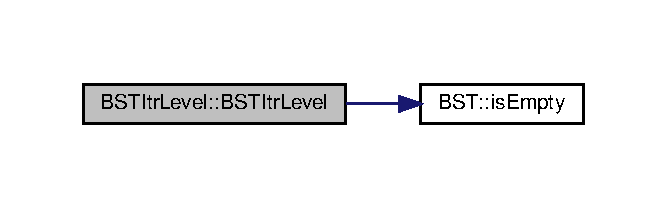
\includegraphics[width=320pt]{classBSTItrLevel_a8fd5cdde93eb182c4cd5cf6b2c5efaeb_cgraph}
\end{center}
\end{figure}


\subsection{Member Function Documentation}
\mbox{\Hypertarget{classBSTItrLevel_ad54a6fa289a59d6050b507abe40d463b}\label{classBSTItrLevel_ad54a6fa289a59d6050b507abe40d463b}} 
\index{B\+S\+T\+Itr\+Level@{B\+S\+T\+Itr\+Level}!advance@{advance}}
\index{advance@{advance}!B\+S\+T\+Itr\+Level@{B\+S\+T\+Itr\+Level}}
\subsubsection{\texorpdfstring{advance()}{advance()}}
{\footnotesize\ttfamily template$<$class Comparable $>$ \\
void \hyperlink{classBSTItrLevel}{B\+S\+T\+Itr\+Level}$<$ Comparable $>$\+::advance (\begin{DoxyParamCaption}{ }\end{DoxyParamCaption})}

\mbox{\Hypertarget{classBSTItrLevel_a89bc8e81dde255fd6bad917cacc0d489}\label{classBSTItrLevel_a89bc8e81dde255fd6bad917cacc0d489}} 
\index{B\+S\+T\+Itr\+Level@{B\+S\+T\+Itr\+Level}!is\+At\+End@{is\+At\+End}}
\index{is\+At\+End@{is\+At\+End}!B\+S\+T\+Itr\+Level@{B\+S\+T\+Itr\+Level}}
\subsubsection{\texorpdfstring{is\+At\+End()}{isAtEnd()}}
{\footnotesize\ttfamily template$<$class Comparable $>$ \\
bool \hyperlink{classBSTItrLevel}{B\+S\+T\+Itr\+Level}$<$ Comparable $>$\+::is\+At\+End (\begin{DoxyParamCaption}{ }\end{DoxyParamCaption})\hspace{0.3cm}{\ttfamily [inline]}}

\mbox{\Hypertarget{classBSTItrLevel_a7932a172129cc6ca14b6efeee1b4dd87}\label{classBSTItrLevel_a7932a172129cc6ca14b6efeee1b4dd87}} 
\index{B\+S\+T\+Itr\+Level@{B\+S\+T\+Itr\+Level}!retrieve@{retrieve}}
\index{retrieve@{retrieve}!B\+S\+T\+Itr\+Level@{B\+S\+T\+Itr\+Level}}
\subsubsection{\texorpdfstring{retrieve()}{retrieve()}}
{\footnotesize\ttfamily template$<$class Comparable $>$ \\
const Comparable\& \hyperlink{classBSTItrLevel}{B\+S\+T\+Itr\+Level}$<$ Comparable $>$\+::retrieve (\begin{DoxyParamCaption}{ }\end{DoxyParamCaption})\hspace{0.3cm}{\ttfamily [inline]}}



\subsection{Member Data Documentation}
\mbox{\Hypertarget{classBSTItrLevel_a6de8f9f3e129e2a358b00ffa35abcb0e}\label{classBSTItrLevel_a6de8f9f3e129e2a358b00ffa35abcb0e}} 
\index{B\+S\+T\+Itr\+Level@{B\+S\+T\+Itr\+Level}!itr\+Queue@{itr\+Queue}}
\index{itr\+Queue@{itr\+Queue}!B\+S\+T\+Itr\+Level@{B\+S\+T\+Itr\+Level}}
\subsubsection{\texorpdfstring{itr\+Queue}{itrQueue}}
{\footnotesize\ttfamily template$<$class Comparable $>$ \\
queue$<$\hyperlink{classBinaryNode}{Binary\+Node}$<$Comparable$>$ $\ast$$>$ \hyperlink{classBSTItrLevel}{B\+S\+T\+Itr\+Level}$<$ Comparable $>$\+::itr\+Queue\hspace{0.3cm}{\ttfamily [private]}}



The documentation for this class was generated from the following file\+:\begin{DoxyCompactItemize}
\item 
src/\hyperlink{BST_8h}{B\+S\+T.\+h}\end{DoxyCompactItemize}

\hypertarget{classBSTItrPost}{}\section{B\+S\+T\+Itr\+Post$<$ Comparable $>$ Class Template Reference}
\label{classBSTItrPost}\index{B\+S\+T\+Itr\+Post$<$ Comparable $>$@{B\+S\+T\+Itr\+Post$<$ Comparable $>$}}


{\ttfamily \#include $<$B\+S\+T.\+h$>$}

\subsection*{Public Member Functions}
\begin{DoxyCompactItemize}
\item 
\hyperlink{classBSTItrPost_acf7e537dea01978f40c40909c55c56c2}{B\+S\+T\+Itr\+Post} (const \hyperlink{classBST}{B\+ST}$<$ Comparable $>$ \&bt)
\item 
void \hyperlink{classBSTItrPost_a376098e5a82cd02118dd4dcdec49bb26}{advance} ()
\item 
const Comparable \& \hyperlink{classBSTItrPost_a1e9f3953f7ae5712bf3c7c6d05059718}{retrieve} ()
\item 
bool \hyperlink{classBSTItrPost_a2f330e73bb817e8bd1c797805e66ddb7}{is\+At\+End} ()
\end{DoxyCompactItemize}
\subsection*{Private Member Functions}
\begin{DoxyCompactItemize}
\item 
void \hyperlink{classBSTItrPost_a56a13ae3a0358eeb06a83d4de745344a}{slide\+Down} (\hyperlink{classBinaryNode}{Binary\+Node}$<$ Comparable $>$ $\ast$n)
\end{DoxyCompactItemize}
\subsection*{Private Attributes}
\begin{DoxyCompactItemize}
\item 
stack$<$ \hyperlink{classBinaryNode}{Binary\+Node}$<$ Comparable $>$ $\ast$ $>$ \hyperlink{classBSTItrPost_add32204909b8a6c3635b926832192ced}{itr\+Stack}
\item 
stack$<$ bool $>$ \hyperlink{classBSTItrPost_a5a9af907c7b135acdf3b5ed9affbb9a7}{visit\+Stack}
\end{DoxyCompactItemize}


\subsection{Constructor \& Destructor Documentation}
\mbox{\Hypertarget{classBSTItrPost_acf7e537dea01978f40c40909c55c56c2}\label{classBSTItrPost_acf7e537dea01978f40c40909c55c56c2}} 
\index{B\+S\+T\+Itr\+Post@{B\+S\+T\+Itr\+Post}!B\+S\+T\+Itr\+Post@{B\+S\+T\+Itr\+Post}}
\index{B\+S\+T\+Itr\+Post@{B\+S\+T\+Itr\+Post}!B\+S\+T\+Itr\+Post@{B\+S\+T\+Itr\+Post}}
\subsubsection{\texorpdfstring{B\+S\+T\+Itr\+Post()}{BSTItrPost()}}
{\footnotesize\ttfamily template$<$class Comparable $>$ \\
\hyperlink{classBSTItrPost}{B\+S\+T\+Itr\+Post}$<$ Comparable $>$\+::\hyperlink{classBSTItrPost}{B\+S\+T\+Itr\+Post} (\begin{DoxyParamCaption}\item[{const \hyperlink{classBST}{B\+ST}$<$ Comparable $>$ \&}]{bt }\end{DoxyParamCaption})}

Here is the call graph for this function\+:\nopagebreak
\begin{figure}[H]
\begin{center}
\leavevmode
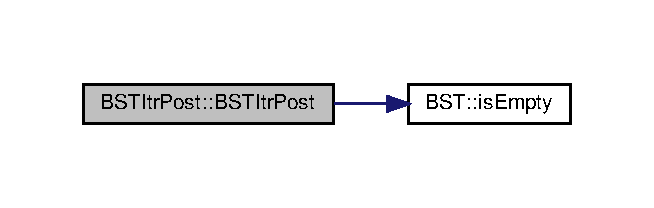
\includegraphics[width=314pt]{classBSTItrPost_acf7e537dea01978f40c40909c55c56c2_cgraph}
\end{center}
\end{figure}


\subsection{Member Function Documentation}
\mbox{\Hypertarget{classBSTItrPost_a376098e5a82cd02118dd4dcdec49bb26}\label{classBSTItrPost_a376098e5a82cd02118dd4dcdec49bb26}} 
\index{B\+S\+T\+Itr\+Post@{B\+S\+T\+Itr\+Post}!advance@{advance}}
\index{advance@{advance}!B\+S\+T\+Itr\+Post@{B\+S\+T\+Itr\+Post}}
\subsubsection{\texorpdfstring{advance()}{advance()}}
{\footnotesize\ttfamily template$<$class Comparable $>$ \\
void \hyperlink{classBSTItrPost}{B\+S\+T\+Itr\+Post}$<$ Comparable $>$\+::advance (\begin{DoxyParamCaption}{ }\end{DoxyParamCaption})}

\mbox{\Hypertarget{classBSTItrPost_a2f330e73bb817e8bd1c797805e66ddb7}\label{classBSTItrPost_a2f330e73bb817e8bd1c797805e66ddb7}} 
\index{B\+S\+T\+Itr\+Post@{B\+S\+T\+Itr\+Post}!is\+At\+End@{is\+At\+End}}
\index{is\+At\+End@{is\+At\+End}!B\+S\+T\+Itr\+Post@{B\+S\+T\+Itr\+Post}}
\subsubsection{\texorpdfstring{is\+At\+End()}{isAtEnd()}}
{\footnotesize\ttfamily template$<$class Comparable $>$ \\
bool \hyperlink{classBSTItrPost}{B\+S\+T\+Itr\+Post}$<$ Comparable $>$\+::is\+At\+End (\begin{DoxyParamCaption}{ }\end{DoxyParamCaption})\hspace{0.3cm}{\ttfamily [inline]}}

\mbox{\Hypertarget{classBSTItrPost_a1e9f3953f7ae5712bf3c7c6d05059718}\label{classBSTItrPost_a1e9f3953f7ae5712bf3c7c6d05059718}} 
\index{B\+S\+T\+Itr\+Post@{B\+S\+T\+Itr\+Post}!retrieve@{retrieve}}
\index{retrieve@{retrieve}!B\+S\+T\+Itr\+Post@{B\+S\+T\+Itr\+Post}}
\subsubsection{\texorpdfstring{retrieve()}{retrieve()}}
{\footnotesize\ttfamily template$<$class Comparable $>$ \\
const Comparable\& \hyperlink{classBSTItrPost}{B\+S\+T\+Itr\+Post}$<$ Comparable $>$\+::retrieve (\begin{DoxyParamCaption}{ }\end{DoxyParamCaption})\hspace{0.3cm}{\ttfamily [inline]}}

\mbox{\Hypertarget{classBSTItrPost_a56a13ae3a0358eeb06a83d4de745344a}\label{classBSTItrPost_a56a13ae3a0358eeb06a83d4de745344a}} 
\index{B\+S\+T\+Itr\+Post@{B\+S\+T\+Itr\+Post}!slide\+Down@{slide\+Down}}
\index{slide\+Down@{slide\+Down}!B\+S\+T\+Itr\+Post@{B\+S\+T\+Itr\+Post}}
\subsubsection{\texorpdfstring{slide\+Down()}{slideDown()}}
{\footnotesize\ttfamily template$<$class Comparable $>$ \\
void \hyperlink{classBSTItrPost}{B\+S\+T\+Itr\+Post}$<$ Comparable $>$\+::slide\+Down (\begin{DoxyParamCaption}\item[{\hyperlink{classBinaryNode}{Binary\+Node}$<$ Comparable $>$ $\ast$}]{n }\end{DoxyParamCaption})\hspace{0.3cm}{\ttfamily [private]}}



\subsection{Member Data Documentation}
\mbox{\Hypertarget{classBSTItrPost_add32204909b8a6c3635b926832192ced}\label{classBSTItrPost_add32204909b8a6c3635b926832192ced}} 
\index{B\+S\+T\+Itr\+Post@{B\+S\+T\+Itr\+Post}!itr\+Stack@{itr\+Stack}}
\index{itr\+Stack@{itr\+Stack}!B\+S\+T\+Itr\+Post@{B\+S\+T\+Itr\+Post}}
\subsubsection{\texorpdfstring{itr\+Stack}{itrStack}}
{\footnotesize\ttfamily template$<$class Comparable $>$ \\
stack$<$\hyperlink{classBinaryNode}{Binary\+Node}$<$Comparable$>$ $\ast$$>$ \hyperlink{classBSTItrPost}{B\+S\+T\+Itr\+Post}$<$ Comparable $>$\+::itr\+Stack\hspace{0.3cm}{\ttfamily [private]}}

\mbox{\Hypertarget{classBSTItrPost_a5a9af907c7b135acdf3b5ed9affbb9a7}\label{classBSTItrPost_a5a9af907c7b135acdf3b5ed9affbb9a7}} 
\index{B\+S\+T\+Itr\+Post@{B\+S\+T\+Itr\+Post}!visit\+Stack@{visit\+Stack}}
\index{visit\+Stack@{visit\+Stack}!B\+S\+T\+Itr\+Post@{B\+S\+T\+Itr\+Post}}
\subsubsection{\texorpdfstring{visit\+Stack}{visitStack}}
{\footnotesize\ttfamily template$<$class Comparable $>$ \\
stack$<$bool$>$ \hyperlink{classBSTItrPost}{B\+S\+T\+Itr\+Post}$<$ Comparable $>$\+::visit\+Stack\hspace{0.3cm}{\ttfamily [private]}}



The documentation for this class was generated from the following file\+:\begin{DoxyCompactItemize}
\item 
src/\hyperlink{BST_8h}{B\+S\+T.\+h}\end{DoxyCompactItemize}

\hypertarget{classBSTItrPre}{}\section{B\+S\+T\+Itr\+Pre$<$ Comparable $>$ Class Template Reference}
\label{classBSTItrPre}\index{B\+S\+T\+Itr\+Pre$<$ Comparable $>$@{B\+S\+T\+Itr\+Pre$<$ Comparable $>$}}


{\ttfamily \#include $<$B\+S\+T.\+h$>$}

\subsection*{Public Member Functions}
\begin{DoxyCompactItemize}
\item 
\hyperlink{classBSTItrPre_a11b1cd4e783f153b9c1b64ce2ec8077e}{B\+S\+T\+Itr\+Pre} (const \hyperlink{classBST}{B\+ST}$<$ Comparable $>$ \&bt)
\item 
void \hyperlink{classBSTItrPre_a7a743d66a842018fd833fb2b0737254d}{advance} ()
\item 
const Comparable \& \hyperlink{classBSTItrPre_ace3c36566d09f71eff8807c9a4fff7fe}{retrieve} ()
\item 
bool \hyperlink{classBSTItrPre_ae282a7b9ffa9d250bb0f6a6d79f6e8d0}{is\+At\+End} ()
\end{DoxyCompactItemize}
\subsection*{Private Attributes}
\begin{DoxyCompactItemize}
\item 
stack$<$ \hyperlink{classBinaryNode}{Binary\+Node}$<$ Comparable $>$ $\ast$ $>$ \hyperlink{classBSTItrPre_a73e938d809acba06490472e7fc1bd6d3}{itr\+Stack}
\end{DoxyCompactItemize}


\subsection{Constructor \& Destructor Documentation}
\mbox{\Hypertarget{classBSTItrPre_a11b1cd4e783f153b9c1b64ce2ec8077e}\label{classBSTItrPre_a11b1cd4e783f153b9c1b64ce2ec8077e}} 
\index{B\+S\+T\+Itr\+Pre@{B\+S\+T\+Itr\+Pre}!B\+S\+T\+Itr\+Pre@{B\+S\+T\+Itr\+Pre}}
\index{B\+S\+T\+Itr\+Pre@{B\+S\+T\+Itr\+Pre}!B\+S\+T\+Itr\+Pre@{B\+S\+T\+Itr\+Pre}}
\subsubsection{\texorpdfstring{B\+S\+T\+Itr\+Pre()}{BSTItrPre()}}
{\footnotesize\ttfamily template$<$class Comparable $>$ \\
\hyperlink{classBSTItrPre}{B\+S\+T\+Itr\+Pre}$<$ Comparable $>$\+::\hyperlink{classBSTItrPre}{B\+S\+T\+Itr\+Pre} (\begin{DoxyParamCaption}\item[{const \hyperlink{classBST}{B\+ST}$<$ Comparable $>$ \&}]{bt }\end{DoxyParamCaption})}

Here is the call graph for this function\+:\nopagebreak
\begin{figure}[H]
\begin{center}
\leavevmode
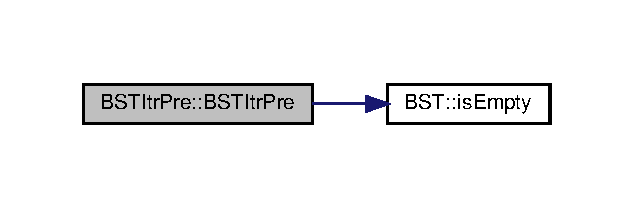
\includegraphics[width=304pt]{classBSTItrPre_a11b1cd4e783f153b9c1b64ce2ec8077e_cgraph}
\end{center}
\end{figure}


\subsection{Member Function Documentation}
\mbox{\Hypertarget{classBSTItrPre_a7a743d66a842018fd833fb2b0737254d}\label{classBSTItrPre_a7a743d66a842018fd833fb2b0737254d}} 
\index{B\+S\+T\+Itr\+Pre@{B\+S\+T\+Itr\+Pre}!advance@{advance}}
\index{advance@{advance}!B\+S\+T\+Itr\+Pre@{B\+S\+T\+Itr\+Pre}}
\subsubsection{\texorpdfstring{advance()}{advance()}}
{\footnotesize\ttfamily template$<$class Comparable $>$ \\
void \hyperlink{classBSTItrPre}{B\+S\+T\+Itr\+Pre}$<$ Comparable $>$\+::advance (\begin{DoxyParamCaption}{ }\end{DoxyParamCaption})}

\mbox{\Hypertarget{classBSTItrPre_ae282a7b9ffa9d250bb0f6a6d79f6e8d0}\label{classBSTItrPre_ae282a7b9ffa9d250bb0f6a6d79f6e8d0}} 
\index{B\+S\+T\+Itr\+Pre@{B\+S\+T\+Itr\+Pre}!is\+At\+End@{is\+At\+End}}
\index{is\+At\+End@{is\+At\+End}!B\+S\+T\+Itr\+Pre@{B\+S\+T\+Itr\+Pre}}
\subsubsection{\texorpdfstring{is\+At\+End()}{isAtEnd()}}
{\footnotesize\ttfamily template$<$class Comparable $>$ \\
bool \hyperlink{classBSTItrPre}{B\+S\+T\+Itr\+Pre}$<$ Comparable $>$\+::is\+At\+End (\begin{DoxyParamCaption}{ }\end{DoxyParamCaption})\hspace{0.3cm}{\ttfamily [inline]}}

\mbox{\Hypertarget{classBSTItrPre_ace3c36566d09f71eff8807c9a4fff7fe}\label{classBSTItrPre_ace3c36566d09f71eff8807c9a4fff7fe}} 
\index{B\+S\+T\+Itr\+Pre@{B\+S\+T\+Itr\+Pre}!retrieve@{retrieve}}
\index{retrieve@{retrieve}!B\+S\+T\+Itr\+Pre@{B\+S\+T\+Itr\+Pre}}
\subsubsection{\texorpdfstring{retrieve()}{retrieve()}}
{\footnotesize\ttfamily template$<$class Comparable $>$ \\
const Comparable\& \hyperlink{classBSTItrPre}{B\+S\+T\+Itr\+Pre}$<$ Comparable $>$\+::retrieve (\begin{DoxyParamCaption}{ }\end{DoxyParamCaption})\hspace{0.3cm}{\ttfamily [inline]}}



\subsection{Member Data Documentation}
\mbox{\Hypertarget{classBSTItrPre_a73e938d809acba06490472e7fc1bd6d3}\label{classBSTItrPre_a73e938d809acba06490472e7fc1bd6d3}} 
\index{B\+S\+T\+Itr\+Pre@{B\+S\+T\+Itr\+Pre}!itr\+Stack@{itr\+Stack}}
\index{itr\+Stack@{itr\+Stack}!B\+S\+T\+Itr\+Pre@{B\+S\+T\+Itr\+Pre}}
\subsubsection{\texorpdfstring{itr\+Stack}{itrStack}}
{\footnotesize\ttfamily template$<$class Comparable $>$ \\
stack$<$\hyperlink{classBinaryNode}{Binary\+Node}$<$Comparable$>$ $\ast$$>$ \hyperlink{classBSTItrPre}{B\+S\+T\+Itr\+Pre}$<$ Comparable $>$\+::itr\+Stack\hspace{0.3cm}{\ttfamily [private]}}



The documentation for this class was generated from the following file\+:\begin{DoxyCompactItemize}
\item 
src/\hyperlink{BST_8h}{B\+S\+T.\+h}\end{DoxyCompactItemize}

\hypertarget{classClient}{}\section{Client Class Reference}
\label{classClient}\index{Client@{Client}}


\hyperlink{classClient}{Client} Class that represents a client.  




{\ttfamily \#include $<$Client.\+h$>$}



Inheritance diagram for Client\+:\nopagebreak
\begin{figure}[H]
\begin{center}
\leavevmode
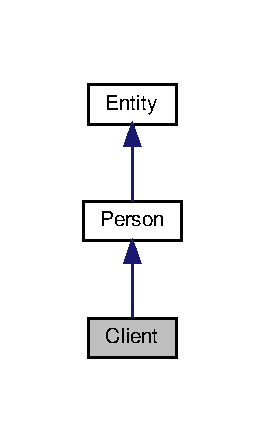
\includegraphics[width=127pt]{classClient__inherit__graph}
\end{center}
\end{figure}


Collaboration diagram for Client\+:\nopagebreak
\begin{figure}[H]
\begin{center}
\leavevmode
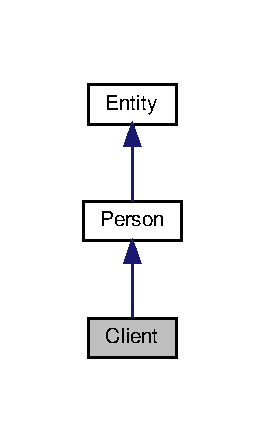
\includegraphics[width=127pt]{classClient__coll__graph}
\end{center}
\end{figure}
\subsection*{Public Member Functions}
\begin{DoxyCompactItemize}
\item 
\hyperlink{classClient_ae054d039da064a80f3bde9e126a58e23}{Client} (string n, string dis, string addr, unsigned int \hyperlink{classPerson_a55eea8ffb71b88d84ea43a6be15a2eb4}{contrib\+No}, vector$<$ unsigned int $>$ \hyperlink{classClient_afceda4b2e1aa4cf7cb52478d5e679bad}{history})
\begin{DoxyCompactList}\small\item\em Construct a new \hyperlink{classClient}{Client} object. \end{DoxyCompactList}\item 
\hyperlink{classClient_ae51af7aa6b8f591496a8f6a4a87a14bf}{Client} ()
\item 
\hyperlink{classClient_a2df8218a19b72961a1301392e356711f}{Client} (unsigned int nc)
\item 
vector$<$ unsigned int $>$ \hyperlink{classClient_a5a2d79bb60bb1846a14263d156654c36}{get\+History} () const
\begin{DoxyCompactList}\small\item\em Get the History object. \end{DoxyCompactList}\item 
bool \hyperlink{classClient_ada079699bae9cf8b0b729c82f0940487}{operator$<$} (const \hyperlink{classClient}{Client} \&c) const
\begin{DoxyCompactList}\small\item\em Operator overload of $<$. \end{DoxyCompactList}\item 
bool \hyperlink{classClient_a7dfa59dc82c7ef516edc0eb6719b97f0}{operator==} (const \hyperlink{classClient}{Client} \&c) const
\begin{DoxyCompactList}\small\item\em Operator overload of ==. \end{DoxyCompactList}\item 
string \hyperlink{classClient_aa6acbbfc2c1717d7303a3db86ac22058}{get\+District} () const
\begin{DoxyCompactList}\small\item\em Get function of the variable district. \end{DoxyCompactList}\end{DoxyCompactItemize}
\subsection*{Private Attributes}
\begin{DoxyCompactItemize}
\item 
vector$<$ unsigned int $>$ \hyperlink{classClient_afceda4b2e1aa4cf7cb52478d5e679bad}{history}
\item 
string \hyperlink{classClient_a4f613c8876f65ad3de6435efc3e9f6a2}{district}
\begin{DoxyCompactList}\small\item\em history of Clients purchases \end{DoxyCompactList}\end{DoxyCompactItemize}
\subsection*{Friends}
\begin{DoxyCompactItemize}
\item 
ostream \& \hyperlink{classClient_ae8980b59fbd6f02e9ebd291446c37bef}{operator$<$$<$} (ostream \&os, const \hyperlink{classClient}{Client} \&c)
\begin{DoxyCompactList}\small\item\em Overload outstream operator $<$$<$ to write a \hyperlink{classClient}{Client} to an outstream. \end{DoxyCompactList}\end{DoxyCompactItemize}


\subsection{Detailed Description}
\hyperlink{classClient}{Client} Class that represents a client. 

\subsection{Constructor \& Destructor Documentation}
\mbox{\Hypertarget{classClient_ae054d039da064a80f3bde9e126a58e23}\label{classClient_ae054d039da064a80f3bde9e126a58e23}} 
\index{Client@{Client}!Client@{Client}}
\index{Client@{Client}!Client@{Client}}
\subsubsection{\texorpdfstring{Client()}{Client()}\hspace{0.1cm}{\footnotesize\ttfamily [1/3]}}
{\footnotesize\ttfamily Client\+::\+Client (\begin{DoxyParamCaption}\item[{string}]{n,  }\item[{string}]{dis,  }\item[{string}]{addr,  }\item[{unsigned int}]{contrib\+No,  }\item[{vector$<$ unsigned int $>$}]{history }\end{DoxyParamCaption})}



Construct a new \hyperlink{classClient}{Client} object. 


\begin{DoxyParams}{Parameters}
{\em n} & The name of the \hyperlink{classClient}{Client} be created \\
\hline
{\em addr} & The adress the \hyperlink{classClient}{Client} be created \\
\hline
{\em contrib\+No} & The tax number of the \hyperlink{classClient}{Client} to be created \\
\hline
\end{DoxyParams}
\mbox{\Hypertarget{classClient_ae51af7aa6b8f591496a8f6a4a87a14bf}\label{classClient_ae51af7aa6b8f591496a8f6a4a87a14bf}} 
\index{Client@{Client}!Client@{Client}}
\index{Client@{Client}!Client@{Client}}
\subsubsection{\texorpdfstring{Client()}{Client()}\hspace{0.1cm}{\footnotesize\ttfamily [2/3]}}
{\footnotesize\ttfamily Client\+::\+Client (\begin{DoxyParamCaption}{ }\end{DoxyParamCaption})}

\mbox{\Hypertarget{classClient_a2df8218a19b72961a1301392e356711f}\label{classClient_a2df8218a19b72961a1301392e356711f}} 
\index{Client@{Client}!Client@{Client}}
\index{Client@{Client}!Client@{Client}}
\subsubsection{\texorpdfstring{Client()}{Client()}\hspace{0.1cm}{\footnotesize\ttfamily [3/3]}}
{\footnotesize\ttfamily Client\+::\+Client (\begin{DoxyParamCaption}\item[{unsigned int}]{nc }\end{DoxyParamCaption})}



\subsection{Member Function Documentation}
\mbox{\Hypertarget{classClient_aa6acbbfc2c1717d7303a3db86ac22058}\label{classClient_aa6acbbfc2c1717d7303a3db86ac22058}} 
\index{Client@{Client}!get\+District@{get\+District}}
\index{get\+District@{get\+District}!Client@{Client}}
\subsubsection{\texorpdfstring{get\+District()}{getDistrict()}}
{\footnotesize\ttfamily string Client\+::get\+District (\begin{DoxyParamCaption}{ }\end{DoxyParamCaption}) const}



Get function of the variable district. 

\begin{DoxyReturn}{Returns}
The district name 
\end{DoxyReturn}
\mbox{\Hypertarget{classClient_a5a2d79bb60bb1846a14263d156654c36}\label{classClient_a5a2d79bb60bb1846a14263d156654c36}} 
\index{Client@{Client}!get\+History@{get\+History}}
\index{get\+History@{get\+History}!Client@{Client}}
\subsubsection{\texorpdfstring{get\+History()}{getHistory()}}
{\footnotesize\ttfamily vector$<$ unsigned int $>$ Client\+::get\+History (\begin{DoxyParamCaption}{ }\end{DoxyParamCaption}) const}



Get the History object. 

\begin{DoxyReturn}{Returns}
vector$<$unsigned int$>$ \hyperlink{classClient}{Client}\textquotesingle{}s purchases history 
\end{DoxyReturn}
\mbox{\Hypertarget{classClient_ada079699bae9cf8b0b729c82f0940487}\label{classClient_ada079699bae9cf8b0b729c82f0940487}} 
\index{Client@{Client}!operator$<$@{operator$<$}}
\index{operator$<$@{operator$<$}!Client@{Client}}
\subsubsection{\texorpdfstring{operator$<$()}{operator<()}}
{\footnotesize\ttfamily bool Client\+::operator$<$ (\begin{DoxyParamCaption}\item[{const \hyperlink{classClient}{Client} \&}]{c }\end{DoxyParamCaption}) const}



Operator overload of $<$. 


\begin{DoxyParams}{Parameters}
{\em c} & \hyperlink{classClient}{Client} to compare this object to\\
\hline
\end{DoxyParams}
\begin{DoxyReturn}{Returns}
Boolean value -\/$>$ true if this object is \char`\"{}smaller\char`\"{} than the other one 
\end{DoxyReturn}
Here is the call graph for this function\+:\nopagebreak
\begin{figure}[H]
\begin{center}
\leavevmode
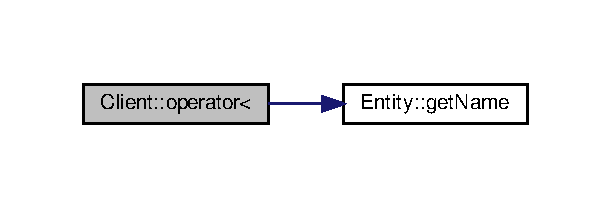
\includegraphics[width=293pt]{classClient_ada079699bae9cf8b0b729c82f0940487_cgraph}
\end{center}
\end{figure}
\mbox{\Hypertarget{classClient_a7dfa59dc82c7ef516edc0eb6719b97f0}\label{classClient_a7dfa59dc82c7ef516edc0eb6719b97f0}} 
\index{Client@{Client}!operator==@{operator==}}
\index{operator==@{operator==}!Client@{Client}}
\subsubsection{\texorpdfstring{operator==()}{operator==()}}
{\footnotesize\ttfamily bool Client\+::operator== (\begin{DoxyParamCaption}\item[{const \hyperlink{classClient}{Client} \&}]{c }\end{DoxyParamCaption}) const}



Operator overload of ==. 


\begin{DoxyParams}{Parameters}
{\em c} & \hyperlink{classClient}{Client} to compare this object to\\
\hline
\end{DoxyParams}
\begin{DoxyReturn}{Returns}
Boolean value -\/$>$ true if both objects are equal 
\end{DoxyReturn}
Here is the call graph for this function\+:\nopagebreak
\begin{figure}[H]
\begin{center}
\leavevmode
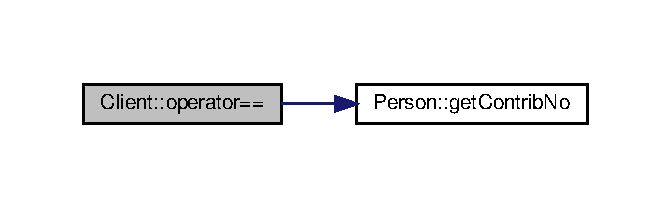
\includegraphics[width=322pt]{classClient_a7dfa59dc82c7ef516edc0eb6719b97f0_cgraph}
\end{center}
\end{figure}


\subsection{Friends And Related Function Documentation}
\mbox{\Hypertarget{classClient_ae8980b59fbd6f02e9ebd291446c37bef}\label{classClient_ae8980b59fbd6f02e9ebd291446c37bef}} 
\index{Client@{Client}!operator$<$$<$@{operator$<$$<$}}
\index{operator$<$$<$@{operator$<$$<$}!Client@{Client}}
\subsubsection{\texorpdfstring{operator$<$$<$}{operator<<}}
{\footnotesize\ttfamily ostream\& operator$<$$<$ (\begin{DoxyParamCaption}\item[{ostream \&}]{os,  }\item[{const \hyperlink{classClient}{Client} \&}]{c }\end{DoxyParamCaption})\hspace{0.3cm}{\ttfamily [friend]}}



Overload outstream operator $<$$<$ to write a \hyperlink{classClient}{Client} to an outstream. 


\begin{DoxyParams}{Parameters}
{\em os} & Outstream\\
\hline
{\em c} & \hyperlink{classClient}{Client} to be written\\
\hline
\end{DoxyParams}
\begin{DoxyReturn}{Returns}
outstream 
\end{DoxyReturn}


\subsection{Member Data Documentation}
\mbox{\Hypertarget{classClient_a4f613c8876f65ad3de6435efc3e9f6a2}\label{classClient_a4f613c8876f65ad3de6435efc3e9f6a2}} 
\index{Client@{Client}!district@{district}}
\index{district@{district}!Client@{Client}}
\subsubsection{\texorpdfstring{district}{district}}
{\footnotesize\ttfamily string Client\+::district\hspace{0.3cm}{\ttfamily [private]}}



history of Clients purchases 

$<$ \mbox{\Hypertarget{classClient_afceda4b2e1aa4cf7cb52478d5e679bad}\label{classClient_afceda4b2e1aa4cf7cb52478d5e679bad}} 
\index{Client@{Client}!history@{history}}
\index{history@{history}!Client@{Client}}
\subsubsection{\texorpdfstring{history}{history}}
{\footnotesize\ttfamily vector$<$unsigned int$>$ Client\+::history\hspace{0.3cm}{\ttfamily [private]}}



The documentation for this class was generated from the following files\+:\begin{DoxyCompactItemize}
\item 
src/\hyperlink{Client_8h}{Client.\+h}\item 
src/\hyperlink{Client_8cpp}{Client.\+cpp}\end{DoxyCompactItemize}

\hypertarget{classDataBase}{}\section{Data\+Base Class Reference}
\label{classDataBase}\index{Data\+Base@{Data\+Base}}


Class containing all the general information and data structures about the other classes.  




{\ttfamily \#include $<$Data\+Base.\+h$>$}



Collaboration diagram for Data\+Base\+:\nopagebreak
\begin{figure}[H]
\begin{center}
\leavevmode
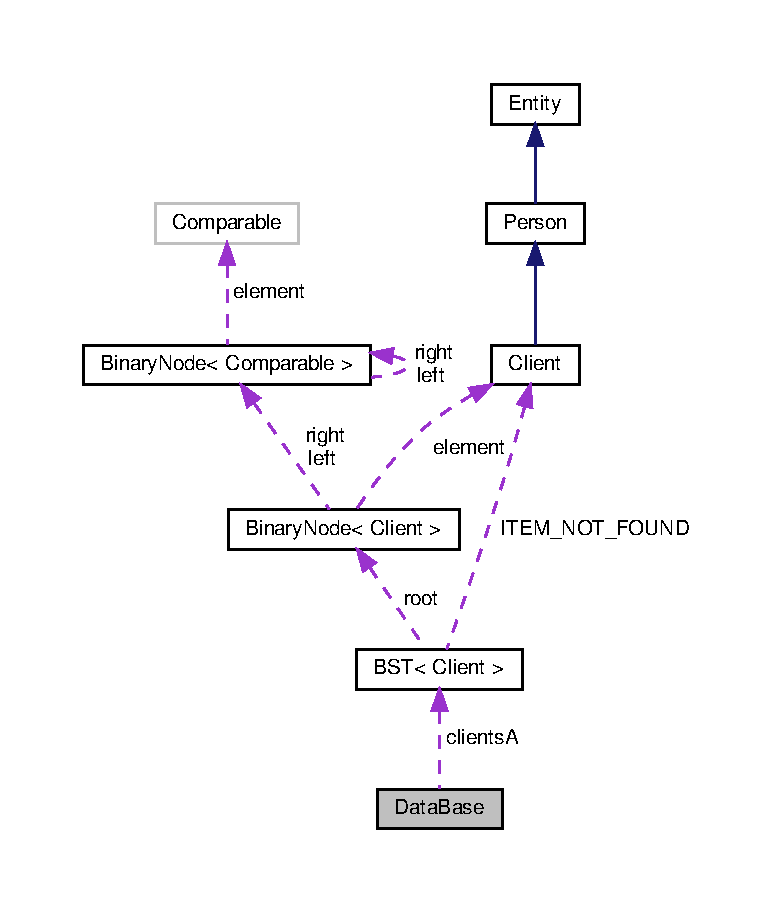
\includegraphics[width=350pt]{classDataBase__coll__graph}
\end{center}
\end{figure}
\subsection*{Public Member Functions}
\begin{DoxyCompactItemize}
\item 
string \hyperlink{classDataBase_ad34d05002555ed7e109fdcfdfbeb70b8}{parsestr} (string in)
\begin{DoxyCompactList}\small\item\em priority queue for the products \end{DoxyCompactList}\item 
void \hyperlink{classDataBase_a6255a0d9489dee6c6de802bcfff2d19e}{less\+Products\+Than} ()
\begin{DoxyCompactList}\small\item\em Checks and displays if there is a product with less products. \end{DoxyCompactList}\item 
bool \hyperlink{classDataBase_a780ad993953bd70eaee64df86d0f1974}{remove\+Quantity} (string name, int quantity)
\item 
\hyperlink{classDataBase_a9fbd4936704ce4de391f92e92a072074}{Data\+Base} ()
\begin{DoxyCompactList}\small\item\em Constructs the \hyperlink{classDataBase}{Data\+Base} object. \end{DoxyCompactList}\item 
\hyperlink{classDataBase_a5a9bd40e9026abb30082e3d0590054d4}{Data\+Base} (string prod\+File, string cli\+File, string pharm\+File, string \hyperlink{classDataBase_a2f564a52132d74186314695a7a0e3270}{staff\+File})
\begin{DoxyCompactList}\small\item\em Constructs the object. \end{DoxyCompactList}\item 
\hyperlink{classDataBase_a5e9a28cc8e7c0d468c8f5bbeaad3a594}{Data\+Base} (string \hyperlink{classDataBase_a24acb8bdda9293336f40a4b08741235e}{products\+File}, string \hyperlink{classDataBase_a7b52741a2183b8b3eba86534d02782e6}{clients\+File}, string \hyperlink{classDataBase_aa52765a56e1fefddb5b1cf638de3493e}{pharmacies\+File}, string \hyperlink{classDataBase_a2f564a52132d74186314695a7a0e3270}{staff\+File}, string \hyperlink{classDataBase_a8b16f4814de788f12e96163255aaa737}{sales\+File}, string \hyperlink{classDataBase_a7649e7e3eda974285c99e78c23829334}{presc\+File})
\begin{DoxyCompactList}\small\item\em Constructs the object. \end{DoxyCompactList}\item 
virtual \hyperlink{classDataBase_a9d4629e705ccaa4897e9650222a2a648}{$\sim$\+Data\+Base} ()
\item 
vector$<$ \hyperlink{classSale}{Sale} $>$ \hyperlink{classDataBase_a0c0c3efb8ee0d6e1a4b2d97b8d35feeb}{get\+Sales} ()
\begin{DoxyCompactList}\small\item\em Gets clients vector. \end{DoxyCompactList}\item 
vector$<$ \hyperlink{classClient}{Client} $>$ \hyperlink{classDataBase_a9ad743bfac0c4b7b4a6f2eaa1d4e8160}{get\+Clients} () const
\item 
vector$<$ \hyperlink{classPharmacy}{Pharmacy} $>$ \hyperlink{classDataBase_a5c7fcbdcc70d9ac4e27188d39b8c9e1a}{get\+Pharmacies} () const
\begin{DoxyCompactList}\small\item\em Gets pharmacies vector. \end{DoxyCompactList}\item 
vector$<$ \hyperlink{classPrescription}{Prescription} $>$ \hyperlink{classDataBase_a2c08363a2f1360996983fdd89760af37}{get\+Prescriptions} () const
\begin{DoxyCompactList}\small\item\em Gets products vector. \end{DoxyCompactList}\item 
vector$<$ \hyperlink{classStaffMember}{Staff\+Member} $>$ \hyperlink{classDataBase_ad44eb614d0001979c6036e57af6b9e06}{get\+Staff} () const
\begin{DoxyCompactList}\small\item\em Gets staff vector. \end{DoxyCompactList}\item 
void \hyperlink{classDataBase_a1eebe53a8f3c83af5d75d3a83590ca01}{add\+Client} ()
\item 
void \hyperlink{classDataBase_a4a6fca7606a5734e623a3d8ea7c00fa4}{add\+Pharmacy} ()
\item 
void \hyperlink{classDataBase_aed28994adfb33442ffd3469496150da8}{add\+Staff\+Member} ()
\item 
void \hyperlink{classDataBase_a0fb00cab402248ffba3903cc1f19f6c2}{add\+Sale} ()
\item 
void \hyperlink{classDataBase_a82e38546b8cb54beffd3185a13a838aa}{add\+Prescription} ()
\item 
void \hyperlink{classDataBase_a654216132c946bdb05ec4ae866302259}{add\+Product} ()
\item 
void \hyperlink{classDataBase_a6be2328441f5fe20086a4f8b0002adee}{remove\+Product} ()
\item 
void \hyperlink{classDataBase_adba6b4fad6dcb329aae27d8f610edaac}{remove\+Sale} ()
\item 
void \hyperlink{classDataBase_a9fb1b3625b3431d09b4b64a13bbb1e0f}{remove\+Client} ()
\item 
void \hyperlink{classDataBase_af923ee9db26814bf9413afe95262a01d}{remove\+Pharmacy} ()
\item 
void \hyperlink{classDataBase_a26ab8f3d2cb6d78a5105e72c2377c21c}{remove\+Staff\+Member} ()
\item 
void \hyperlink{classDataBase_af4762294e1b25415f7de88f0e8d6d90f}{show\+All\+Clients} ()
\item 
void \hyperlink{classDataBase_ab00290f55389cd62d8ee5594ecf9a6b5}{show\+All\+Pharmacies} ()
\item 
void \hyperlink{classDataBase_aa1d2ae05f581ec45eb8da06e468aec30}{show\+All\+Staff} ()
\item 
void \hyperlink{classDataBase_abf8a64bd81ce3207862b0105d52f646f}{show\+All\+Sales} ()
\item 
void \hyperlink{classDataBase_a40a951f6f2c923ca315655956ab8e196}{show\+All\+Prescriptions} ()
\item 
void \hyperlink{classDataBase_a74dcc435917c328bd89aaf5fd3cb804d}{show\+All\+Products} ()
\item 
void \hyperlink{classDataBase_a32341ca202561239807fb5b3a1f96d13}{read\+Products\+File} ()
\item 
\hyperlink{classProduct}{Product} \hyperlink{classDataBase_ae83d4c612ff8d93b69ab1c05345cd62c}{get\+Product\+By\+Name} (string name)
\item 
void \hyperlink{classDataBase_a514959070d22346ea7ee212e51cab89f}{open\+Clients\+File} ()
\item 
void \hyperlink{classDataBase_a30cd564502803b00dbe575b0bd9376e6}{open\+Pharmacies\+File} ()
\item 
void \hyperlink{classDataBase_a22f0ad79cc0d695ac5c4cfb3c556f920}{open\+Staff\+File} ()
\item 
void \hyperlink{classDataBase_abcf98b385e2a76f71b602e791699dbb3}{open\+Products\+File} ()
\item 
void \hyperlink{classDataBase_a5b7842d4ca431e2edb592fadc16da4c6}{open\+Sales\+File} ()
\item 
void \hyperlink{classDataBase_a10c16844e17eae108e828390a92fb3b8}{open\+Prescription\+File} ()
\item 
void \hyperlink{classDataBase_a4d855ccf967f4f741646100d2c890ede}{write\+To\+Clients\+File} ()
\item 
void \hyperlink{classDataBase_aef0dc00d9d40159c361518e60e78f857}{write\+To\+Pharmacies\+File} ()
\item 
void \hyperlink{classDataBase_abc8c8d3116c6b3422d87ae781ba91538}{write\+To\+Staff\+File} ()
\item 
void \hyperlink{classDataBase_a62cb54f7bbcd213d71f604003298cd95}{write\+To\+Sales\+File} ()
\item 
void \hyperlink{classDataBase_a108ba0eb315d14ed6bc7181b98499318}{write\+To\+Products\+File} ()
\item 
void \hyperlink{classDataBase_a1435e1728598586503f199981b84a933}{write\+To\+Prescription\+File} ()
\item 
string \hyperlink{classDataBase_aa7cfe42e76e1d57c0adfb82d0c82f96e}{parse} (string in)
\item 
string \hyperlink{classDataBase_ae547604cf1c5a0c937139928a3a700b5}{parse\+Staff} (string in)
\item 
string \hyperlink{classDataBase_a5310a888c5c94fc87135b5cf8b9267f5}{parse\+Product\+Sale} (string sale)
\item 
string \hyperlink{classDataBase_ab0744d4be63a6db44fdcf21c22d61914}{parse\+Product} (string in)
\item 
\hyperlink{classStaffMember}{Staff\+Member} $\ast$ \hyperlink{classDataBase_af3c7f6a88b927dbd01b34121eefabe4d}{get\+StaffM} (string name)
\begin{DoxyCompactList}\small\item\em Gets the staff Member with name name. \end{DoxyCompactList}\item 
\hyperlink{classSale}{Sale} \hyperlink{classDataBase_af233d5e69141c780d6a7946b1810a7a6}{get\+Sale} (unsigned int code)
\begin{DoxyCompactList}\small\item\em Gets the sala with code code. \end{DoxyCompactList}\item 
tm \hyperlink{classDataBase_aa63ea6b1a96135acd1839ae9a0983d3f}{parse\+Date} (string in)
\item 
void \hyperlink{classDataBase_a0bf85b7fb0feb4fb1f6888ba58ebe2b2}{write\+To\+Sales} (string file\+Name)
\begin{DoxyCompactList}\small\item\em Writes the info saved in the \hyperlink{classDataBase}{Data\+Base} to the Sales file. \end{DoxyCompactList}\item 
{\footnotesize template$<$class T $>$ }\\void \hyperlink{classDataBase_a136d789db1f6c1cd615dc1bdbe27557b}{write\+To\+FileW} (string file\+Name, vector$<$ T $>$ v)
\item 
void \hyperlink{classDataBase_aec542d0eb4b2c2d44abe5cefd25d2057}{write\+To\+Products\+File2} (string file\+Name)
\item 
void \hyperlink{classDataBase_a0c83992321a456f8fa097ea5bbf4a093}{show\+All\+ClientsA} ()
\begin{DoxyCompactList}\small\item\em Displays all the clients in the \hyperlink{classDataBase}{Data\+Base}. \end{DoxyCompactList}\item 
void \hyperlink{classDataBase_a2016794a78b86df19676ea9aba3114bc}{show\+Clients\+By\+District} ()
\begin{DoxyCompactList}\small\item\em Displays all clients from a specific district. \end{DoxyCompactList}\item 
void \hyperlink{classDataBase_aa613181e1960fa22305feae26560960b}{get\+Client\+Info} ()
\begin{DoxyCompactList}\small\item\em Displays the client with specific id info. \end{DoxyCompactList}\item 
\hyperlink{classClient}{Client} \hyperlink{classDataBase_a8575c65a7f0d76352e4b37604562fbc2}{client\+Exists} (unsigned int nc)
\begin{DoxyCompactList}\small\item\em Looks for a \hyperlink{classClient}{Client} in the \hyperlink{classDataBase}{Data\+Base} with specific id and returns it. \end{DoxyCompactList}\item 
void \hyperlink{classDataBase_ab87e9a50f26c934790774b0bf0d62a51}{show\+Clients\+With\+Most\+Purchases} ()
\begin{DoxyCompactList}\small\item\em Displays the clients on the top 3 of most purchases made. \end{DoxyCompactList}\item 
void \hyperlink{classDataBase_aecde8e08249b522ff9431c9feed57996}{assign\+Staff} (vector$<$ \hyperlink{classStaffMember}{Staff\+Member} $>$ members)
\begin{DoxyCompactList}\small\item\em Asks the user to assign some \hyperlink{classStaffMember}{Staff\+Member} \textquotesingle{}s to existing \hyperlink{classPharmacy}{Pharmacy} \textquotesingle{}s. \end{DoxyCompactList}\item 
void \hyperlink{classDataBase_a28237a8f74d11c092cf250d17c7997f1}{assign\+Staff\+With\+No\+Ph} ()
\begin{DoxyCompactList}\small\item\em Asks the user to assign all \hyperlink{classStaffMember}{Staff\+Member} \textquotesingle{}s in the \hyperlink{classDataBase}{Data\+Base} with no \hyperlink{classPharmacy}{Pharmacy} assigned. \end{DoxyCompactList}\item 
void \hyperlink{classDataBase_ab17fba12d1810b3548615b3ac0427850}{show\+Staff\+Without\+Ph} ()
\begin{DoxyCompactList}\small\item\em Displays all \hyperlink{classStaffMember}{Staff\+Member} \textquotesingle{}s in the \hyperlink{classDataBase}{Data\+Base} with no \hyperlink{classPharmacy}{Pharmacy} assigned. \end{DoxyCompactList}\item 
string \hyperlink{classDataBase_a33b218c5674029a4696a44d710f88aa6}{check\+Ph\+Name} ()
\begin{DoxyCompactList}\small\item\em Keeps asking the user for the name of a \hyperlink{classPharmacy}{Pharmacy} until an existing one is given. \end{DoxyCompactList}\item 
void \hyperlink{classDataBase_ac572ac9a3091e0adcef16ab79bfba7fb}{show\+Pharmacies\+Names} ()
\begin{DoxyCompactList}\small\item\em Displays the names of the pharmacies available in the DB. \end{DoxyCompactList}\item 
void \hyperlink{classDataBase_a9704dec1b0797bf3f6dc18a754a4a1b5}{change\+Pharmacy\+Info} ()
\begin{DoxyCompactList}\small\item\em Asks the user edit a \hyperlink{classPharmacy}{Pharmacy} \textquotesingle{}s info. \end{DoxyCompactList}\item 
void \hyperlink{classDataBase_a79dbf45f9b1a60fd5a29505f44e188e0}{remove\+StaffM} (string name)
\begin{DoxyCompactList}\small\item\em Searches through pharmacies vector and removes the \hyperlink{classStaffMember}{Staff\+Member} with a specific name from one of those pharmacies. \end{DoxyCompactList}\item 
void \hyperlink{classDataBase_a85445c22323399e318780faf36854c2f}{staff\+Ph\+To\+None} (string name)
\end{DoxyCompactItemize}
\subsection*{Private Attributes}
\begin{DoxyCompactItemize}
\item 
string \hyperlink{classDataBase_a7649e7e3eda974285c99e78c23829334}{presc\+File}
\item 
string \hyperlink{classDataBase_a24acb8bdda9293336f40a4b08741235e}{products\+File}
\item 
string \hyperlink{classDataBase_a7b52741a2183b8b3eba86534d02782e6}{clients\+File}
\item 
string \hyperlink{classDataBase_aa52765a56e1fefddb5b1cf638de3493e}{pharmacies\+File}
\item 
string \hyperlink{classDataBase_a2f564a52132d74186314695a7a0e3270}{staff\+File}
\item 
string \hyperlink{classDataBase_a8b16f4814de788f12e96163255aaa737}{sales\+File}
\item 
\hyperlink{DataBase_8h_a309f0ca910338932f751c46c6e5ccbbc}{files\+HT} \hyperlink{classDataBase_a576f0eac012d39fffb1064a5ea27ad08}{files}
\begin{DoxyCompactList}\small\item\em files names \end{DoxyCompactList}\item 
vector$<$ \hyperlink{classClient}{Client} $>$ \hyperlink{classDataBase_aa5f93e5229c216c200681b551db2db77}{clients}
\item 
vector$<$ \hyperlink{classPharmacy}{Pharmacy} $>$ \hyperlink{classDataBase_ada5f113e22144b1b28775557e2a10f08}{pharmacies}
\begin{DoxyCompactList}\small\item\em vector for clients \end{DoxyCompactList}\item 
vector$<$ \hyperlink{classStaffMember}{Staff\+Member} $>$ \hyperlink{classDataBase_a74729cf98d5b60cc2bfbac6c0fa00229}{staff}
\begin{DoxyCompactList}\small\item\em vector for pharmacies \end{DoxyCompactList}\item 
vector$<$ \hyperlink{classPrescription}{Prescription} $>$ \hyperlink{classDataBase_a592b7e885d6708309c298406db68c505}{prescriptions}
\begin{DoxyCompactList}\small\item\em vector for staff \end{DoxyCompactList}\item 
vector$<$ \hyperlink{classSale}{Sale} $>$ \hyperlink{classDataBase_a4e48e9c0e840c7f9febf3344c5a003ba}{sales}
\begin{DoxyCompactList}\small\item\em vector for prescriptions \end{DoxyCompactList}\item 
\hyperlink{classBST}{B\+ST}$<$ \hyperlink{classClient}{Client} $>$ \hyperlink{classDataBase_a9b3973c4282ee24f7769f4f735b4b898}{clientsA}
\begin{DoxyCompactList}\small\item\em vector for sales \end{DoxyCompactList}\item 
priority\+\_\+queue$<$ \hyperlink{classProduct}{Product} $>$ \hyperlink{classDataBase_a83dd84eb12b869e3e585fe965c414eef}{products}
\begin{DoxyCompactList}\small\item\em \hyperlink{classBST}{B\+ST} for the clients. \end{DoxyCompactList}\end{DoxyCompactItemize}


\subsection{Detailed Description}
Class containing all the general information and data structures about the other classes. 

\subsection{Constructor \& Destructor Documentation}
\mbox{\Hypertarget{classDataBase_a9fbd4936704ce4de391f92e92a072074}\label{classDataBase_a9fbd4936704ce4de391f92e92a072074}} 
\index{Data\+Base@{Data\+Base}!Data\+Base@{Data\+Base}}
\index{Data\+Base@{Data\+Base}!Data\+Base@{Data\+Base}}
\subsubsection{\texorpdfstring{Data\+Base()}{DataBase()}\hspace{0.1cm}{\footnotesize\ttfamily [1/3]}}
{\footnotesize\ttfamily Data\+Base\+::\+Data\+Base (\begin{DoxyParamCaption}{ }\end{DoxyParamCaption})}



Constructs the \hyperlink{classDataBase}{Data\+Base} object. 

\mbox{\Hypertarget{classDataBase_a5a9bd40e9026abb30082e3d0590054d4}\label{classDataBase_a5a9bd40e9026abb30082e3d0590054d4}} 
\index{Data\+Base@{Data\+Base}!Data\+Base@{Data\+Base}}
\index{Data\+Base@{Data\+Base}!Data\+Base@{Data\+Base}}
\subsubsection{\texorpdfstring{Data\+Base()}{DataBase()}\hspace{0.1cm}{\footnotesize\ttfamily [2/3]}}
{\footnotesize\ttfamily Data\+Base\+::\+Data\+Base (\begin{DoxyParamCaption}\item[{string}]{prod\+File,  }\item[{string}]{cli\+File,  }\item[{string}]{pharm\+File,  }\item[{string}]{staff\+File }\end{DoxyParamCaption})}



Constructs the object. 


\begin{DoxyParams}{Parameters}
{\em prod\+File} & products File\\
\hline
{\em cli\+File} & clients File\\
\hline
{\em pharm\+File} & pharmacies File\\
\hline
{\em staff\+File} & staff File \\
\hline
\end{DoxyParams}
\mbox{\Hypertarget{classDataBase_a5e9a28cc8e7c0d468c8f5bbeaad3a594}\label{classDataBase_a5e9a28cc8e7c0d468c8f5bbeaad3a594}} 
\index{Data\+Base@{Data\+Base}!Data\+Base@{Data\+Base}}
\index{Data\+Base@{Data\+Base}!Data\+Base@{Data\+Base}}
\subsubsection{\texorpdfstring{Data\+Base()}{DataBase()}\hspace{0.1cm}{\footnotesize\ttfamily [3/3]}}
{\footnotesize\ttfamily Data\+Base\+::\+Data\+Base (\begin{DoxyParamCaption}\item[{string}]{products\+File,  }\item[{string}]{clients\+File,  }\item[{string}]{pharmacies\+File,  }\item[{string}]{staff\+File,  }\item[{string}]{sales\+File,  }\item[{string}]{presc\+File }\end{DoxyParamCaption})}



Constructs the object. 


\begin{DoxyParams}{Parameters}
{\em products\+File} & products File\\
\hline
{\em clients\+File} & clients File\\
\hline
{\em pharmacies\+File} & pharmacies File\\
\hline
{\em staff\+File} & staff File\\
\hline
{\em sales\+File} & sales File\\
\hline
{\em presc\+File} & prescriptions File \\
\hline
\end{DoxyParams}
Here is the call graph for this function\+:\nopagebreak
\begin{figure}[H]
\begin{center}
\leavevmode
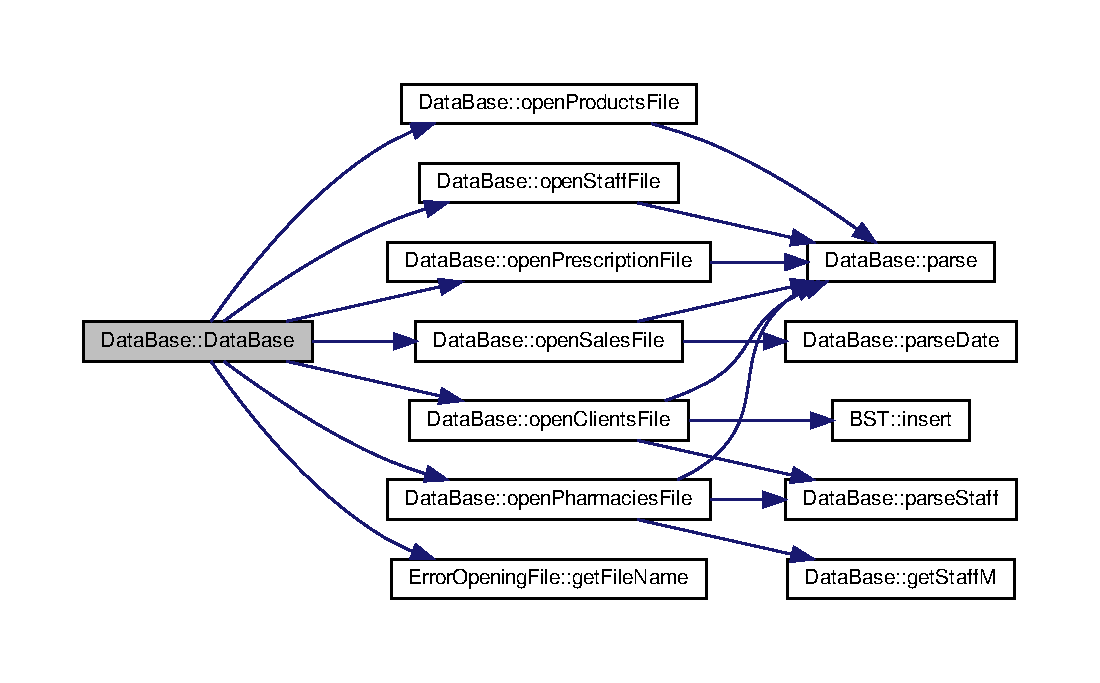
\includegraphics[width=350pt]{classDataBase_a5e9a28cc8e7c0d468c8f5bbeaad3a594_cgraph}
\end{center}
\end{figure}
\mbox{\Hypertarget{classDataBase_a9d4629e705ccaa4897e9650222a2a648}\label{classDataBase_a9d4629e705ccaa4897e9650222a2a648}} 
\index{Data\+Base@{Data\+Base}!````~Data\+Base@{$\sim$\+Data\+Base}}
\index{````~Data\+Base@{$\sim$\+Data\+Base}!Data\+Base@{Data\+Base}}
\subsubsection{\texorpdfstring{$\sim$\+Data\+Base()}{~DataBase()}}
{\footnotesize\ttfamily Data\+Base\+::$\sim$\+Data\+Base (\begin{DoxyParamCaption}{ }\end{DoxyParamCaption})\hspace{0.3cm}{\ttfamily [virtual]}}



\subsection{Member Function Documentation}
\mbox{\Hypertarget{classDataBase_a1eebe53a8f3c83af5d75d3a83590ca01}\label{classDataBase_a1eebe53a8f3c83af5d75d3a83590ca01}} 
\index{Data\+Base@{Data\+Base}!add\+Client@{add\+Client}}
\index{add\+Client@{add\+Client}!Data\+Base@{Data\+Base}}
\subsubsection{\texorpdfstring{add\+Client()}{addClient()}}
{\footnotesize\ttfamily void Data\+Base\+::add\+Client (\begin{DoxyParamCaption}{ }\end{DoxyParamCaption})}

Here is the call graph for this function\+:\nopagebreak
\begin{figure}[H]
\begin{center}
\leavevmode
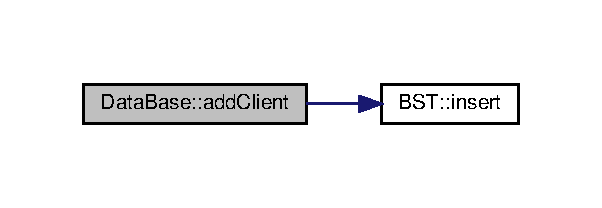
\includegraphics[width=289pt]{classDataBase_a1eebe53a8f3c83af5d75d3a83590ca01_cgraph}
\end{center}
\end{figure}
\mbox{\Hypertarget{classDataBase_a4a6fca7606a5734e623a3d8ea7c00fa4}\label{classDataBase_a4a6fca7606a5734e623a3d8ea7c00fa4}} 
\index{Data\+Base@{Data\+Base}!add\+Pharmacy@{add\+Pharmacy}}
\index{add\+Pharmacy@{add\+Pharmacy}!Data\+Base@{Data\+Base}}
\subsubsection{\texorpdfstring{add\+Pharmacy()}{addPharmacy()}}
{\footnotesize\ttfamily void Data\+Base\+::add\+Pharmacy (\begin{DoxyParamCaption}{ }\end{DoxyParamCaption})}

\mbox{\Hypertarget{classDataBase_a82e38546b8cb54beffd3185a13a838aa}\label{classDataBase_a82e38546b8cb54beffd3185a13a838aa}} 
\index{Data\+Base@{Data\+Base}!add\+Prescription@{add\+Prescription}}
\index{add\+Prescription@{add\+Prescription}!Data\+Base@{Data\+Base}}
\subsubsection{\texorpdfstring{add\+Prescription()}{addPrescription()}}
{\footnotesize\ttfamily void Data\+Base\+::add\+Prescription (\begin{DoxyParamCaption}{ }\end{DoxyParamCaption})}

\mbox{\Hypertarget{classDataBase_a654216132c946bdb05ec4ae866302259}\label{classDataBase_a654216132c946bdb05ec4ae866302259}} 
\index{Data\+Base@{Data\+Base}!add\+Product@{add\+Product}}
\index{add\+Product@{add\+Product}!Data\+Base@{Data\+Base}}
\subsubsection{\texorpdfstring{add\+Product()}{addProduct()}}
{\footnotesize\ttfamily void Data\+Base\+::add\+Product (\begin{DoxyParamCaption}{ }\end{DoxyParamCaption})}

\mbox{\Hypertarget{classDataBase_a0fb00cab402248ffba3903cc1f19f6c2}\label{classDataBase_a0fb00cab402248ffba3903cc1f19f6c2}} 
\index{Data\+Base@{Data\+Base}!add\+Sale@{add\+Sale}}
\index{add\+Sale@{add\+Sale}!Data\+Base@{Data\+Base}}
\subsubsection{\texorpdfstring{add\+Sale()}{addSale()}}
{\footnotesize\ttfamily void Data\+Base\+::add\+Sale (\begin{DoxyParamCaption}{ }\end{DoxyParamCaption})}

Here is the call graph for this function\+:\nopagebreak
\begin{figure}[H]
\begin{center}
\leavevmode
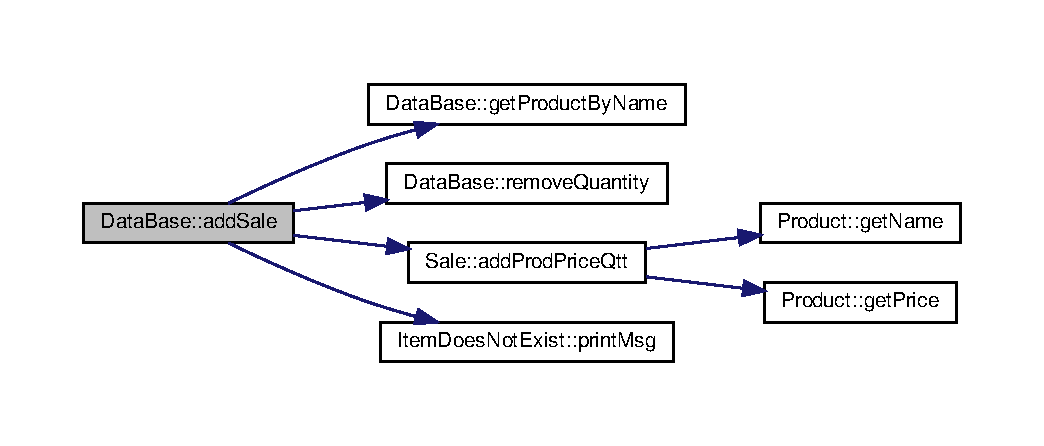
\includegraphics[width=350pt]{classDataBase_a0fb00cab402248ffba3903cc1f19f6c2_cgraph}
\end{center}
\end{figure}
\mbox{\Hypertarget{classDataBase_aed28994adfb33442ffd3469496150da8}\label{classDataBase_aed28994adfb33442ffd3469496150da8}} 
\index{Data\+Base@{Data\+Base}!add\+Staff\+Member@{add\+Staff\+Member}}
\index{add\+Staff\+Member@{add\+Staff\+Member}!Data\+Base@{Data\+Base}}
\subsubsection{\texorpdfstring{add\+Staff\+Member()}{addStaffMember()}}
{\footnotesize\ttfamily void Data\+Base\+::add\+Staff\+Member (\begin{DoxyParamCaption}{ }\end{DoxyParamCaption})}

Here is the call graph for this function\+:\nopagebreak
\begin{figure}[H]
\begin{center}
\leavevmode
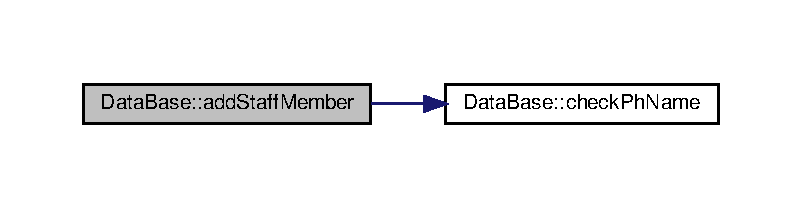
\includegraphics[width=350pt]{classDataBase_aed28994adfb33442ffd3469496150da8_cgraph}
\end{center}
\end{figure}
\mbox{\Hypertarget{classDataBase_aecde8e08249b522ff9431c9feed57996}\label{classDataBase_aecde8e08249b522ff9431c9feed57996}} 
\index{Data\+Base@{Data\+Base}!assign\+Staff@{assign\+Staff}}
\index{assign\+Staff@{assign\+Staff}!Data\+Base@{Data\+Base}}
\subsubsection{\texorpdfstring{assign\+Staff()}{assignStaff()}}
{\footnotesize\ttfamily void Data\+Base\+::assign\+Staff (\begin{DoxyParamCaption}\item[{vector$<$ \hyperlink{classStaffMember}{Staff\+Member} $>$}]{members }\end{DoxyParamCaption})}



Asks the user to assign some \hyperlink{classStaffMember}{Staff\+Member} \textquotesingle{}s to existing \hyperlink{classPharmacy}{Pharmacy} \textquotesingle{}s. 


\begin{DoxyParams}{Parameters}
{\em members} & Vector containing the \hyperlink{classStaffMember}{Staff\+Member} \textquotesingle{}s to be assigned \\
\hline
\end{DoxyParams}
Here is the call graph for this function\+:\nopagebreak
\begin{figure}[H]
\begin{center}
\leavevmode
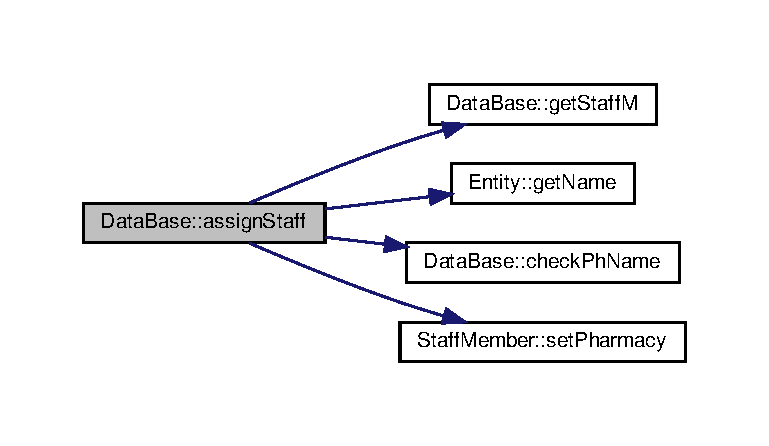
\includegraphics[width=350pt]{classDataBase_aecde8e08249b522ff9431c9feed57996_cgraph}
\end{center}
\end{figure}
\mbox{\Hypertarget{classDataBase_a28237a8f74d11c092cf250d17c7997f1}\label{classDataBase_a28237a8f74d11c092cf250d17c7997f1}} 
\index{Data\+Base@{Data\+Base}!assign\+Staff\+With\+No\+Ph@{assign\+Staff\+With\+No\+Ph}}
\index{assign\+Staff\+With\+No\+Ph@{assign\+Staff\+With\+No\+Ph}!Data\+Base@{Data\+Base}}
\subsubsection{\texorpdfstring{assign\+Staff\+With\+No\+Ph()}{assignStaffWithNoPh()}}
{\footnotesize\ttfamily void Data\+Base\+::assign\+Staff\+With\+No\+Ph (\begin{DoxyParamCaption}{ }\end{DoxyParamCaption})}



Asks the user to assign all \hyperlink{classStaffMember}{Staff\+Member} \textquotesingle{}s in the \hyperlink{classDataBase}{Data\+Base} with no \hyperlink{classPharmacy}{Pharmacy} assigned. 

Here is the call graph for this function\+:\nopagebreak
\begin{figure}[H]
\begin{center}
\leavevmode
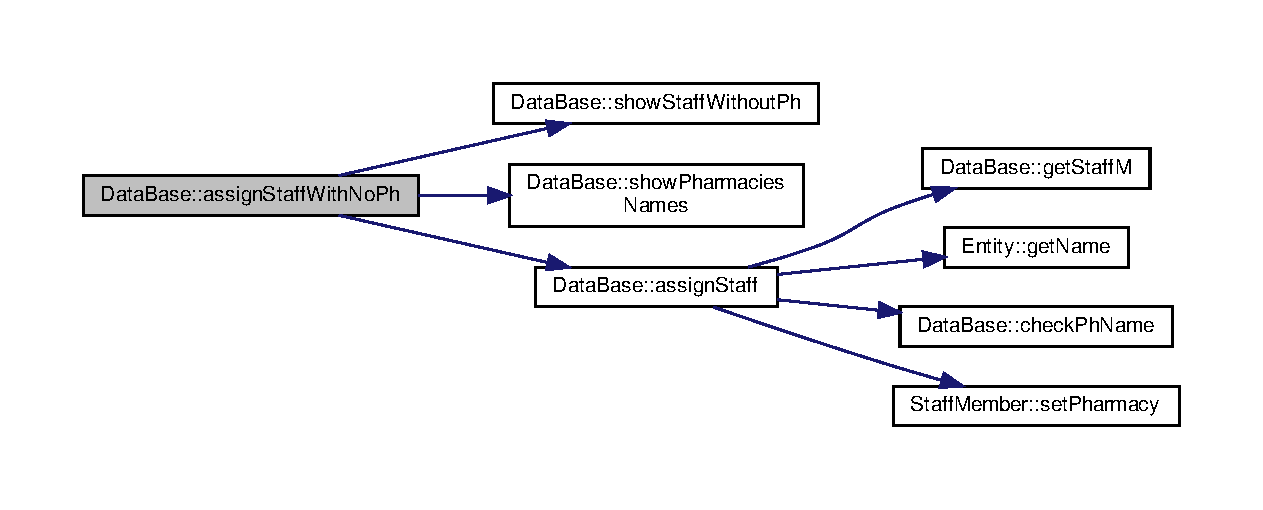
\includegraphics[width=350pt]{classDataBase_a28237a8f74d11c092cf250d17c7997f1_cgraph}
\end{center}
\end{figure}
\mbox{\Hypertarget{classDataBase_a9704dec1b0797bf3f6dc18a754a4a1b5}\label{classDataBase_a9704dec1b0797bf3f6dc18a754a4a1b5}} 
\index{Data\+Base@{Data\+Base}!change\+Pharmacy\+Info@{change\+Pharmacy\+Info}}
\index{change\+Pharmacy\+Info@{change\+Pharmacy\+Info}!Data\+Base@{Data\+Base}}
\subsubsection{\texorpdfstring{change\+Pharmacy\+Info()}{changePharmacyInfo()}}
{\footnotesize\ttfamily void Data\+Base\+::change\+Pharmacy\+Info (\begin{DoxyParamCaption}{ }\end{DoxyParamCaption})}



Asks the user edit a \hyperlink{classPharmacy}{Pharmacy} \textquotesingle{}s info. 

Here is the call graph for this function\+:\nopagebreak
\begin{figure}[H]
\begin{center}
\leavevmode
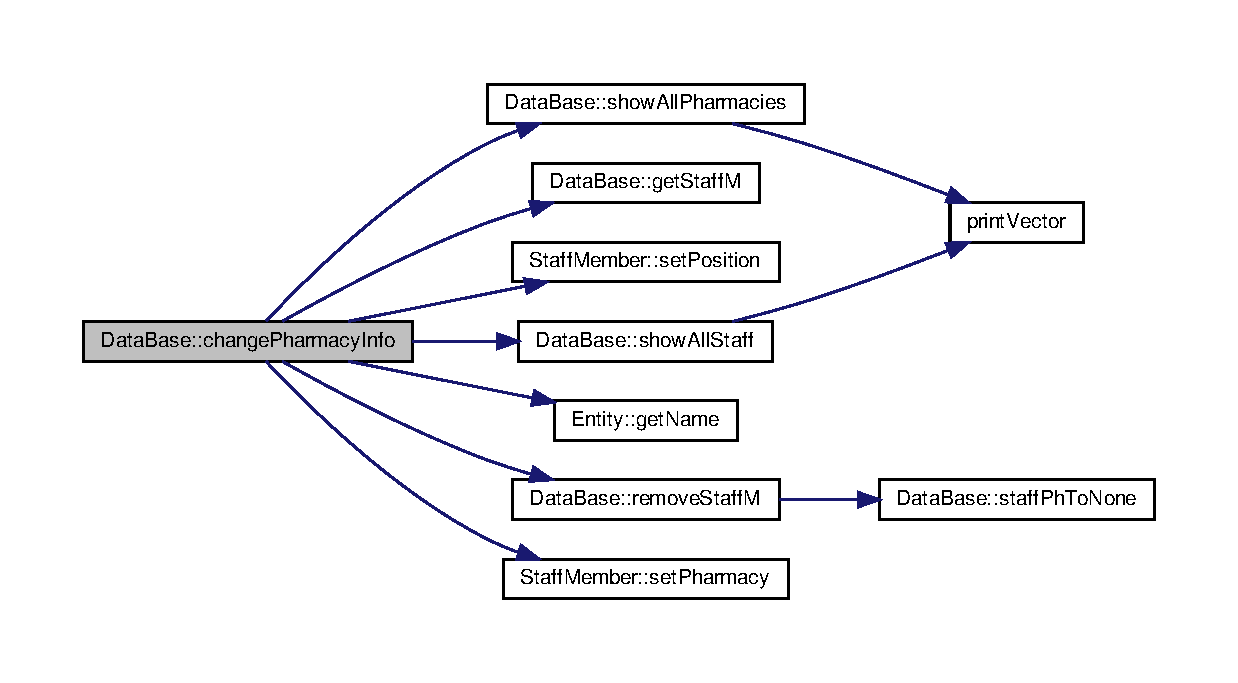
\includegraphics[width=350pt]{classDataBase_a9704dec1b0797bf3f6dc18a754a4a1b5_cgraph}
\end{center}
\end{figure}
\mbox{\Hypertarget{classDataBase_a33b218c5674029a4696a44d710f88aa6}\label{classDataBase_a33b218c5674029a4696a44d710f88aa6}} 
\index{Data\+Base@{Data\+Base}!check\+Ph\+Name@{check\+Ph\+Name}}
\index{check\+Ph\+Name@{check\+Ph\+Name}!Data\+Base@{Data\+Base}}
\subsubsection{\texorpdfstring{check\+Ph\+Name()}{checkPhName()}}
{\footnotesize\ttfamily string Data\+Base\+::check\+Ph\+Name (\begin{DoxyParamCaption}{ }\end{DoxyParamCaption})}



Keeps asking the user for the name of a \hyperlink{classPharmacy}{Pharmacy} until an existing one is given. 

return String with an existing \hyperlink{classPharmacy}{Pharmacy} name \mbox{\Hypertarget{classDataBase_a8575c65a7f0d76352e4b37604562fbc2}\label{classDataBase_a8575c65a7f0d76352e4b37604562fbc2}} 
\index{Data\+Base@{Data\+Base}!client\+Exists@{client\+Exists}}
\index{client\+Exists@{client\+Exists}!Data\+Base@{Data\+Base}}
\subsubsection{\texorpdfstring{client\+Exists()}{clientExists()}}
{\footnotesize\ttfamily \hyperlink{classClient}{Client} Data\+Base\+::client\+Exists (\begin{DoxyParamCaption}\item[{unsigned int}]{nc }\end{DoxyParamCaption})}



Looks for a \hyperlink{classClient}{Client} in the \hyperlink{classDataBase}{Data\+Base} with specific id and returns it. 


\begin{DoxyParams}{Parameters}
{\em nc} & Id of the \hyperlink{classClient}{Client}\\
\hline
\end{DoxyParams}
\begin{DoxyReturn}{Returns}
The \hyperlink{classClient}{Client} object we want to get 
\end{DoxyReturn}
Here is the call graph for this function\+:\nopagebreak
\begin{figure}[H]
\begin{center}
\leavevmode
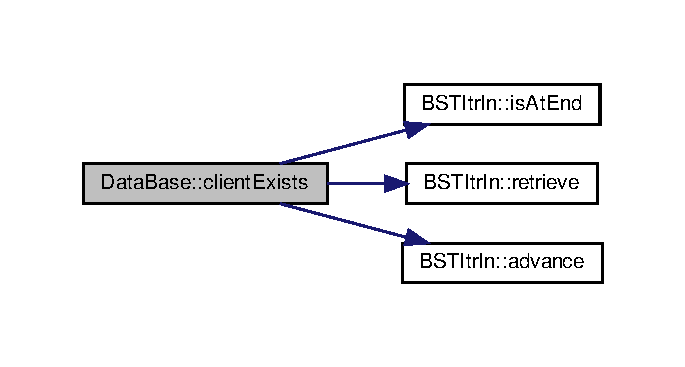
\includegraphics[width=329pt]{classDataBase_a8575c65a7f0d76352e4b37604562fbc2_cgraph}
\end{center}
\end{figure}
\mbox{\Hypertarget{classDataBase_aa613181e1960fa22305feae26560960b}\label{classDataBase_aa613181e1960fa22305feae26560960b}} 
\index{Data\+Base@{Data\+Base}!get\+Client\+Info@{get\+Client\+Info}}
\index{get\+Client\+Info@{get\+Client\+Info}!Data\+Base@{Data\+Base}}
\subsubsection{\texorpdfstring{get\+Client\+Info()}{getClientInfo()}}
{\footnotesize\ttfamily void Data\+Base\+::get\+Client\+Info (\begin{DoxyParamCaption}{ }\end{DoxyParamCaption})}



Displays the client with specific id info. 


\begin{DoxyParams}{Parameters}
{\em nc} & Id of the client \\
\hline
\end{DoxyParams}
Here is the call graph for this function\+:\nopagebreak
\begin{figure}[H]
\begin{center}
\leavevmode
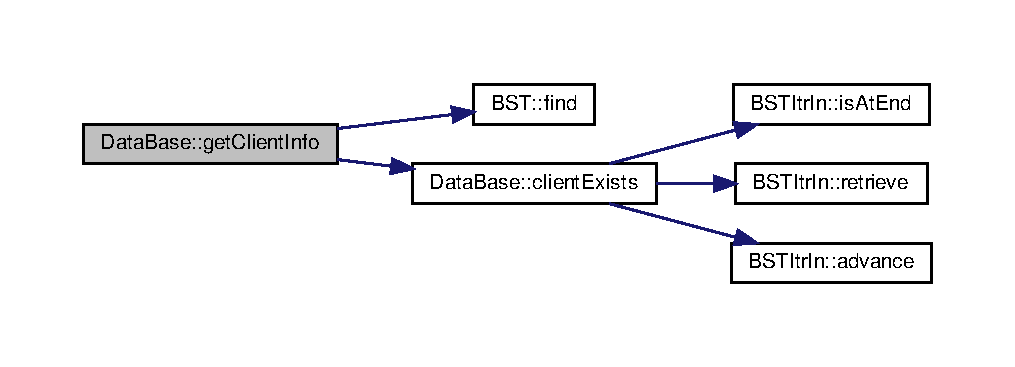
\includegraphics[width=350pt]{classDataBase_aa613181e1960fa22305feae26560960b_cgraph}
\end{center}
\end{figure}
\mbox{\Hypertarget{classDataBase_a9ad743bfac0c4b7b4a6f2eaa1d4e8160}\label{classDataBase_a9ad743bfac0c4b7b4a6f2eaa1d4e8160}} 
\index{Data\+Base@{Data\+Base}!get\+Clients@{get\+Clients}}
\index{get\+Clients@{get\+Clients}!Data\+Base@{Data\+Base}}
\subsubsection{\texorpdfstring{get\+Clients()}{getClients()}}
{\footnotesize\ttfamily vector$<$ \hyperlink{classClient}{Client} $>$ Data\+Base\+::get\+Clients (\begin{DoxyParamCaption}{ }\end{DoxyParamCaption}) const}

\mbox{\Hypertarget{classDataBase_a5c7fcbdcc70d9ac4e27188d39b8c9e1a}\label{classDataBase_a5c7fcbdcc70d9ac4e27188d39b8c9e1a}} 
\index{Data\+Base@{Data\+Base}!get\+Pharmacies@{get\+Pharmacies}}
\index{get\+Pharmacies@{get\+Pharmacies}!Data\+Base@{Data\+Base}}
\subsubsection{\texorpdfstring{get\+Pharmacies()}{getPharmacies()}}
{\footnotesize\ttfamily vector$<$ \hyperlink{classPharmacy}{Pharmacy} $>$ Data\+Base\+::get\+Pharmacies (\begin{DoxyParamCaption}{ }\end{DoxyParamCaption}) const}



Gets pharmacies vector. 

\mbox{\Hypertarget{classDataBase_a2c08363a2f1360996983fdd89760af37}\label{classDataBase_a2c08363a2f1360996983fdd89760af37}} 
\index{Data\+Base@{Data\+Base}!get\+Prescriptions@{get\+Prescriptions}}
\index{get\+Prescriptions@{get\+Prescriptions}!Data\+Base@{Data\+Base}}
\subsubsection{\texorpdfstring{get\+Prescriptions()}{getPrescriptions()}}
{\footnotesize\ttfamily vector$<$ \hyperlink{classPrescription}{Prescription} $>$ Data\+Base\+::get\+Prescriptions (\begin{DoxyParamCaption}{ }\end{DoxyParamCaption}) const}



Gets products vector. 

Gets prescriptions vector \mbox{\Hypertarget{classDataBase_ae83d4c612ff8d93b69ab1c05345cd62c}\label{classDataBase_ae83d4c612ff8d93b69ab1c05345cd62c}} 
\index{Data\+Base@{Data\+Base}!get\+Product\+By\+Name@{get\+Product\+By\+Name}}
\index{get\+Product\+By\+Name@{get\+Product\+By\+Name}!Data\+Base@{Data\+Base}}
\subsubsection{\texorpdfstring{get\+Product\+By\+Name()}{getProductByName()}}
{\footnotesize\ttfamily \hyperlink{classProduct}{Product} Data\+Base\+::get\+Product\+By\+Name (\begin{DoxyParamCaption}\item[{string}]{name }\end{DoxyParamCaption})}

\mbox{\Hypertarget{classDataBase_af233d5e69141c780d6a7946b1810a7a6}\label{classDataBase_af233d5e69141c780d6a7946b1810a7a6}} 
\index{Data\+Base@{Data\+Base}!get\+Sale@{get\+Sale}}
\index{get\+Sale@{get\+Sale}!Data\+Base@{Data\+Base}}
\subsubsection{\texorpdfstring{get\+Sale()}{getSale()}}
{\footnotesize\ttfamily \hyperlink{classSale}{Sale} Data\+Base\+::get\+Sale (\begin{DoxyParamCaption}\item[{unsigned int}]{code }\end{DoxyParamCaption})}



Gets the sala with code code. 


\begin{DoxyParams}{Parameters}
{\em code} & The code\\
\hline
\end{DoxyParams}
\begin{DoxyReturn}{Returns}
The staff code. 
\end{DoxyReturn}
\mbox{\Hypertarget{classDataBase_a0c0c3efb8ee0d6e1a4b2d97b8d35feeb}\label{classDataBase_a0c0c3efb8ee0d6e1a4b2d97b8d35feeb}} 
\index{Data\+Base@{Data\+Base}!get\+Sales@{get\+Sales}}
\index{get\+Sales@{get\+Sales}!Data\+Base@{Data\+Base}}
\subsubsection{\texorpdfstring{get\+Sales()}{getSales()}}
{\footnotesize\ttfamily vector$<$\hyperlink{classSale}{Sale}$>$ Data\+Base\+::get\+Sales (\begin{DoxyParamCaption}{ }\end{DoxyParamCaption})\hspace{0.3cm}{\ttfamily [inline]}}



Gets clients vector. 

\mbox{\Hypertarget{classDataBase_ad44eb614d0001979c6036e57af6b9e06}\label{classDataBase_ad44eb614d0001979c6036e57af6b9e06}} 
\index{Data\+Base@{Data\+Base}!get\+Staff@{get\+Staff}}
\index{get\+Staff@{get\+Staff}!Data\+Base@{Data\+Base}}
\subsubsection{\texorpdfstring{get\+Staff()}{getStaff()}}
{\footnotesize\ttfamily vector$<$ \hyperlink{classStaffMember}{Staff\+Member} $>$ Data\+Base\+::get\+Staff (\begin{DoxyParamCaption}{ }\end{DoxyParamCaption}) const}



Gets staff vector. 

\mbox{\Hypertarget{classDataBase_af3c7f6a88b927dbd01b34121eefabe4d}\label{classDataBase_af3c7f6a88b927dbd01b34121eefabe4d}} 
\index{Data\+Base@{Data\+Base}!get\+StaffM@{get\+StaffM}}
\index{get\+StaffM@{get\+StaffM}!Data\+Base@{Data\+Base}}
\subsubsection{\texorpdfstring{get\+Staff\+M()}{getStaffM()}}
{\footnotesize\ttfamily \hyperlink{classStaffMember}{Staff\+Member} $\ast$ Data\+Base\+::get\+StaffM (\begin{DoxyParamCaption}\item[{string}]{name }\end{DoxyParamCaption})}



Gets the staff Member with name name. 


\begin{DoxyParams}{Parameters}
{\em name} & The name\\
\hline
\end{DoxyParams}
\begin{DoxyReturn}{Returns}
The staff member. 
\end{DoxyReturn}
\mbox{\Hypertarget{classDataBase_a6255a0d9489dee6c6de802bcfff2d19e}\label{classDataBase_a6255a0d9489dee6c6de802bcfff2d19e}} 
\index{Data\+Base@{Data\+Base}!less\+Products\+Than@{less\+Products\+Than}}
\index{less\+Products\+Than@{less\+Products\+Than}!Data\+Base@{Data\+Base}}
\subsubsection{\texorpdfstring{less\+Products\+Than()}{lessProductsThan()}}
{\footnotesize\ttfamily void Data\+Base\+::less\+Products\+Than (\begin{DoxyParamCaption}{ }\end{DoxyParamCaption})}



Checks and displays if there is a product with less products. 

\mbox{\Hypertarget{classDataBase_a514959070d22346ea7ee212e51cab89f}\label{classDataBase_a514959070d22346ea7ee212e51cab89f}} 
\index{Data\+Base@{Data\+Base}!open\+Clients\+File@{open\+Clients\+File}}
\index{open\+Clients\+File@{open\+Clients\+File}!Data\+Base@{Data\+Base}}
\subsubsection{\texorpdfstring{open\+Clients\+File()}{openClientsFile()}}
{\footnotesize\ttfamily void Data\+Base\+::open\+Clients\+File (\begin{DoxyParamCaption}{ }\end{DoxyParamCaption})}

Here is the call graph for this function\+:\nopagebreak
\begin{figure}[H]
\begin{center}
\leavevmode
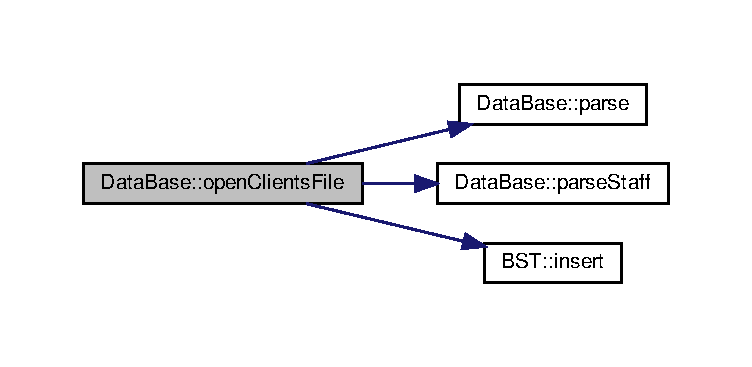
\includegraphics[width=350pt]{classDataBase_a514959070d22346ea7ee212e51cab89f_cgraph}
\end{center}
\end{figure}
\mbox{\Hypertarget{classDataBase_a30cd564502803b00dbe575b0bd9376e6}\label{classDataBase_a30cd564502803b00dbe575b0bd9376e6}} 
\index{Data\+Base@{Data\+Base}!open\+Pharmacies\+File@{open\+Pharmacies\+File}}
\index{open\+Pharmacies\+File@{open\+Pharmacies\+File}!Data\+Base@{Data\+Base}}
\subsubsection{\texorpdfstring{open\+Pharmacies\+File()}{openPharmaciesFile()}}
{\footnotesize\ttfamily void Data\+Base\+::open\+Pharmacies\+File (\begin{DoxyParamCaption}{ }\end{DoxyParamCaption})}

Here is the call graph for this function\+:\nopagebreak
\begin{figure}[H]
\begin{center}
\leavevmode
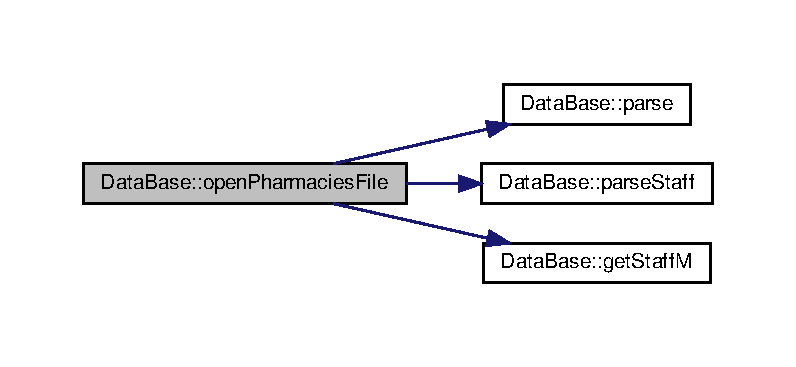
\includegraphics[width=350pt]{classDataBase_a30cd564502803b00dbe575b0bd9376e6_cgraph}
\end{center}
\end{figure}
\mbox{\Hypertarget{classDataBase_a10c16844e17eae108e828390a92fb3b8}\label{classDataBase_a10c16844e17eae108e828390a92fb3b8}} 
\index{Data\+Base@{Data\+Base}!open\+Prescription\+File@{open\+Prescription\+File}}
\index{open\+Prescription\+File@{open\+Prescription\+File}!Data\+Base@{Data\+Base}}
\subsubsection{\texorpdfstring{open\+Prescription\+File()}{openPrescriptionFile()}}
{\footnotesize\ttfamily void Data\+Base\+::open\+Prescription\+File (\begin{DoxyParamCaption}{ }\end{DoxyParamCaption})}

Here is the call graph for this function\+:\nopagebreak
\begin{figure}[H]
\begin{center}
\leavevmode
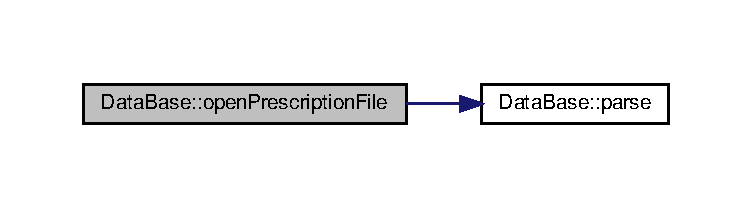
\includegraphics[width=350pt]{classDataBase_a10c16844e17eae108e828390a92fb3b8_cgraph}
\end{center}
\end{figure}
\mbox{\Hypertarget{classDataBase_abcf98b385e2a76f71b602e791699dbb3}\label{classDataBase_abcf98b385e2a76f71b602e791699dbb3}} 
\index{Data\+Base@{Data\+Base}!open\+Products\+File@{open\+Products\+File}}
\index{open\+Products\+File@{open\+Products\+File}!Data\+Base@{Data\+Base}}
\subsubsection{\texorpdfstring{open\+Products\+File()}{openProductsFile()}}
{\footnotesize\ttfamily void Data\+Base\+::open\+Products\+File (\begin{DoxyParamCaption}{ }\end{DoxyParamCaption})}

Here is the call graph for this function\+:\nopagebreak
\begin{figure}[H]
\begin{center}
\leavevmode
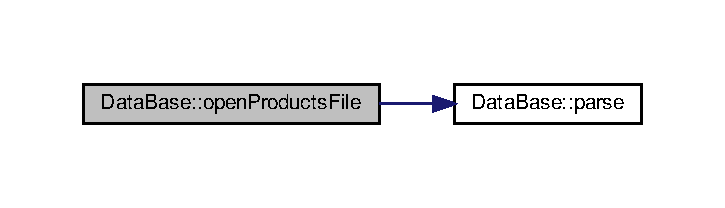
\includegraphics[width=348pt]{classDataBase_abcf98b385e2a76f71b602e791699dbb3_cgraph}
\end{center}
\end{figure}
\mbox{\Hypertarget{classDataBase_a5b7842d4ca431e2edb592fadc16da4c6}\label{classDataBase_a5b7842d4ca431e2edb592fadc16da4c6}} 
\index{Data\+Base@{Data\+Base}!open\+Sales\+File@{open\+Sales\+File}}
\index{open\+Sales\+File@{open\+Sales\+File}!Data\+Base@{Data\+Base}}
\subsubsection{\texorpdfstring{open\+Sales\+File()}{openSalesFile()}}
{\footnotesize\ttfamily void Data\+Base\+::open\+Sales\+File (\begin{DoxyParamCaption}{ }\end{DoxyParamCaption})}

Here is the call graph for this function\+:\nopagebreak
\begin{figure}[H]
\begin{center}
\leavevmode
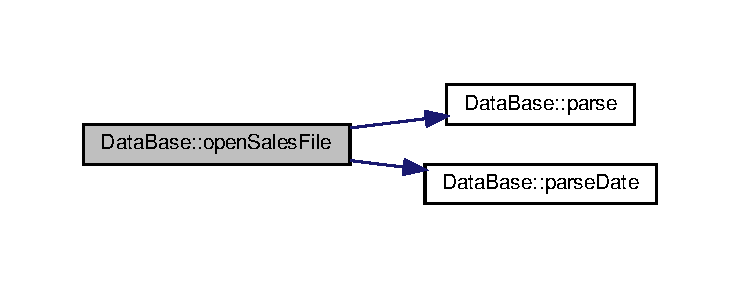
\includegraphics[width=350pt]{classDataBase_a5b7842d4ca431e2edb592fadc16da4c6_cgraph}
\end{center}
\end{figure}
\mbox{\Hypertarget{classDataBase_a22f0ad79cc0d695ac5c4cfb3c556f920}\label{classDataBase_a22f0ad79cc0d695ac5c4cfb3c556f920}} 
\index{Data\+Base@{Data\+Base}!open\+Staff\+File@{open\+Staff\+File}}
\index{open\+Staff\+File@{open\+Staff\+File}!Data\+Base@{Data\+Base}}
\subsubsection{\texorpdfstring{open\+Staff\+File()}{openStaffFile()}}
{\footnotesize\ttfamily void Data\+Base\+::open\+Staff\+File (\begin{DoxyParamCaption}{ }\end{DoxyParamCaption})}

Here is the call graph for this function\+:\nopagebreak
\begin{figure}[H]
\begin{center}
\leavevmode
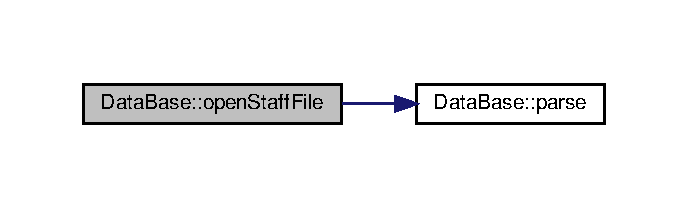
\includegraphics[width=330pt]{classDataBase_a22f0ad79cc0d695ac5c4cfb3c556f920_cgraph}
\end{center}
\end{figure}
\mbox{\Hypertarget{classDataBase_aa7cfe42e76e1d57c0adfb82d0c82f96e}\label{classDataBase_aa7cfe42e76e1d57c0adfb82d0c82f96e}} 
\index{Data\+Base@{Data\+Base}!parse@{parse}}
\index{parse@{parse}!Data\+Base@{Data\+Base}}
\subsubsection{\texorpdfstring{parse()}{parse()}}
{\footnotesize\ttfamily string Data\+Base\+::parse (\begin{DoxyParamCaption}\item[{string}]{in }\end{DoxyParamCaption})}

\mbox{\Hypertarget{classDataBase_aa63ea6b1a96135acd1839ae9a0983d3f}\label{classDataBase_aa63ea6b1a96135acd1839ae9a0983d3f}} 
\index{Data\+Base@{Data\+Base}!parse\+Date@{parse\+Date}}
\index{parse\+Date@{parse\+Date}!Data\+Base@{Data\+Base}}
\subsubsection{\texorpdfstring{parse\+Date()}{parseDate()}}
{\footnotesize\ttfamily tm Data\+Base\+::parse\+Date (\begin{DoxyParamCaption}\item[{string}]{in }\end{DoxyParamCaption})}

\mbox{\Hypertarget{classDataBase_ab0744d4be63a6db44fdcf21c22d61914}\label{classDataBase_ab0744d4be63a6db44fdcf21c22d61914}} 
\index{Data\+Base@{Data\+Base}!parse\+Product@{parse\+Product}}
\index{parse\+Product@{parse\+Product}!Data\+Base@{Data\+Base}}
\subsubsection{\texorpdfstring{parse\+Product()}{parseProduct()}}
{\footnotesize\ttfamily string Data\+Base\+::parse\+Product (\begin{DoxyParamCaption}\item[{string}]{in }\end{DoxyParamCaption})}

\mbox{\Hypertarget{classDataBase_a5310a888c5c94fc87135b5cf8b9267f5}\label{classDataBase_a5310a888c5c94fc87135b5cf8b9267f5}} 
\index{Data\+Base@{Data\+Base}!parse\+Product\+Sale@{parse\+Product\+Sale}}
\index{parse\+Product\+Sale@{parse\+Product\+Sale}!Data\+Base@{Data\+Base}}
\subsubsection{\texorpdfstring{parse\+Product\+Sale()}{parseProductSale()}}
{\footnotesize\ttfamily string Data\+Base\+::parse\+Product\+Sale (\begin{DoxyParamCaption}\item[{string}]{sale }\end{DoxyParamCaption})}

\mbox{\Hypertarget{classDataBase_ae547604cf1c5a0c937139928a3a700b5}\label{classDataBase_ae547604cf1c5a0c937139928a3a700b5}} 
\index{Data\+Base@{Data\+Base}!parse\+Staff@{parse\+Staff}}
\index{parse\+Staff@{parse\+Staff}!Data\+Base@{Data\+Base}}
\subsubsection{\texorpdfstring{parse\+Staff()}{parseStaff()}}
{\footnotesize\ttfamily string Data\+Base\+::parse\+Staff (\begin{DoxyParamCaption}\item[{string}]{in }\end{DoxyParamCaption})}

\mbox{\Hypertarget{classDataBase_ad34d05002555ed7e109fdcfdfbeb70b8}\label{classDataBase_ad34d05002555ed7e109fdcfdfbeb70b8}} 
\index{Data\+Base@{Data\+Base}!parsestr@{parsestr}}
\index{parsestr@{parsestr}!Data\+Base@{Data\+Base}}
\subsubsection{\texorpdfstring{parsestr()}{parsestr()}}
{\footnotesize\ttfamily string Data\+Base\+::parsestr (\begin{DoxyParamCaption}\item[{string}]{in }\end{DoxyParamCaption})}



priority queue for the products 

\mbox{\Hypertarget{classDataBase_a32341ca202561239807fb5b3a1f96d13}\label{classDataBase_a32341ca202561239807fb5b3a1f96d13}} 
\index{Data\+Base@{Data\+Base}!read\+Products\+File@{read\+Products\+File}}
\index{read\+Products\+File@{read\+Products\+File}!Data\+Base@{Data\+Base}}
\subsubsection{\texorpdfstring{read\+Products\+File()}{readProductsFile()}}
{\footnotesize\ttfamily void Data\+Base\+::read\+Products\+File (\begin{DoxyParamCaption}{ }\end{DoxyParamCaption})}

\mbox{\Hypertarget{classDataBase_a9fb1b3625b3431d09b4b64a13bbb1e0f}\label{classDataBase_a9fb1b3625b3431d09b4b64a13bbb1e0f}} 
\index{Data\+Base@{Data\+Base}!remove\+Client@{remove\+Client}}
\index{remove\+Client@{remove\+Client}!Data\+Base@{Data\+Base}}
\subsubsection{\texorpdfstring{remove\+Client()}{removeClient()}}
{\footnotesize\ttfamily void Data\+Base\+::remove\+Client (\begin{DoxyParamCaption}{ }\end{DoxyParamCaption})}

Here is the call graph for this function\+:\nopagebreak
\begin{figure}[H]
\begin{center}
\leavevmode
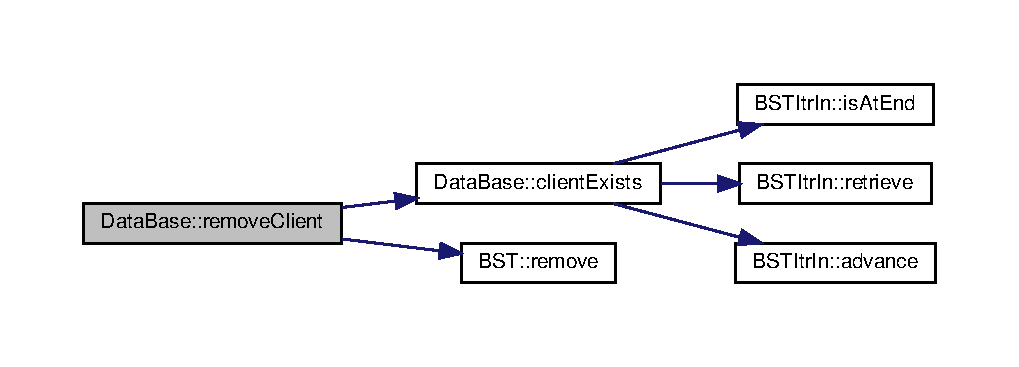
\includegraphics[width=350pt]{classDataBase_a9fb1b3625b3431d09b4b64a13bbb1e0f_cgraph}
\end{center}
\end{figure}
\mbox{\Hypertarget{classDataBase_af923ee9db26814bf9413afe95262a01d}\label{classDataBase_af923ee9db26814bf9413afe95262a01d}} 
\index{Data\+Base@{Data\+Base}!remove\+Pharmacy@{remove\+Pharmacy}}
\index{remove\+Pharmacy@{remove\+Pharmacy}!Data\+Base@{Data\+Base}}
\subsubsection{\texorpdfstring{remove\+Pharmacy()}{removePharmacy()}}
{\footnotesize\ttfamily void Data\+Base\+::remove\+Pharmacy (\begin{DoxyParamCaption}{ }\end{DoxyParamCaption})}

Here is the call graph for this function\+:\nopagebreak
\begin{figure}[H]
\begin{center}
\leavevmode
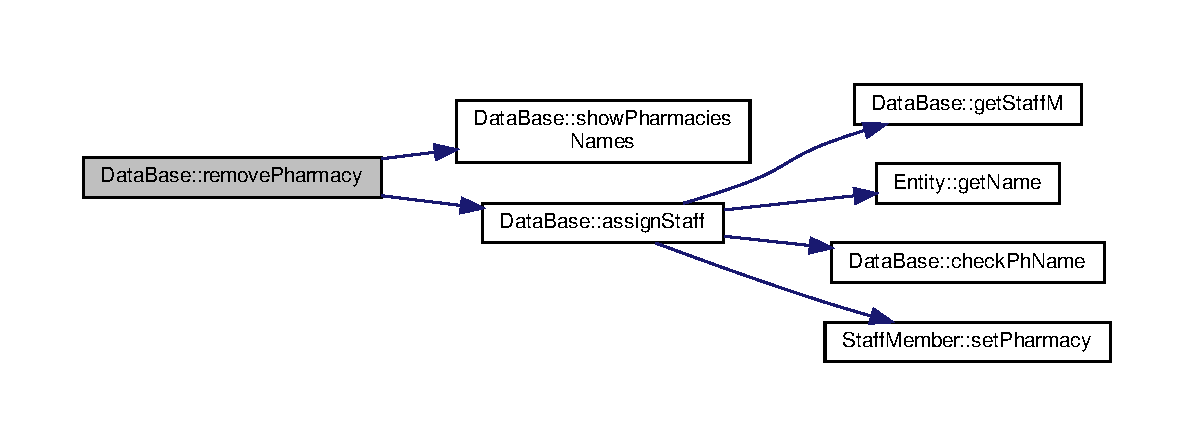
\includegraphics[width=350pt]{classDataBase_af923ee9db26814bf9413afe95262a01d_cgraph}
\end{center}
\end{figure}
\mbox{\Hypertarget{classDataBase_a6be2328441f5fe20086a4f8b0002adee}\label{classDataBase_a6be2328441f5fe20086a4f8b0002adee}} 
\index{Data\+Base@{Data\+Base}!remove\+Product@{remove\+Product}}
\index{remove\+Product@{remove\+Product}!Data\+Base@{Data\+Base}}
\subsubsection{\texorpdfstring{remove\+Product()}{removeProduct()}}
{\footnotesize\ttfamily void Data\+Base\+::remove\+Product (\begin{DoxyParamCaption}{ }\end{DoxyParamCaption})}

\mbox{\Hypertarget{classDataBase_a780ad993953bd70eaee64df86d0f1974}\label{classDataBase_a780ad993953bd70eaee64df86d0f1974}} 
\index{Data\+Base@{Data\+Base}!remove\+Quantity@{remove\+Quantity}}
\index{remove\+Quantity@{remove\+Quantity}!Data\+Base@{Data\+Base}}
\subsubsection{\texorpdfstring{remove\+Quantity()}{removeQuantity()}}
{\footnotesize\ttfamily bool Data\+Base\+::remove\+Quantity (\begin{DoxyParamCaption}\item[{string}]{name,  }\item[{int}]{quantity }\end{DoxyParamCaption})}

\mbox{\Hypertarget{classDataBase_adba6b4fad6dcb329aae27d8f610edaac}\label{classDataBase_adba6b4fad6dcb329aae27d8f610edaac}} 
\index{Data\+Base@{Data\+Base}!remove\+Sale@{remove\+Sale}}
\index{remove\+Sale@{remove\+Sale}!Data\+Base@{Data\+Base}}
\subsubsection{\texorpdfstring{remove\+Sale()}{removeSale()}}
{\footnotesize\ttfamily void Data\+Base\+::remove\+Sale (\begin{DoxyParamCaption}{ }\end{DoxyParamCaption})}

\mbox{\Hypertarget{classDataBase_a79dbf45f9b1a60fd5a29505f44e188e0}\label{classDataBase_a79dbf45f9b1a60fd5a29505f44e188e0}} 
\index{Data\+Base@{Data\+Base}!remove\+StaffM@{remove\+StaffM}}
\index{remove\+StaffM@{remove\+StaffM}!Data\+Base@{Data\+Base}}
\subsubsection{\texorpdfstring{remove\+Staff\+M()}{removeStaffM()}}
{\footnotesize\ttfamily void Data\+Base\+::remove\+StaffM (\begin{DoxyParamCaption}\item[{string}]{name }\end{DoxyParamCaption})}



Searches through pharmacies vector and removes the \hyperlink{classStaffMember}{Staff\+Member} with a specific name from one of those pharmacies. 


\begin{DoxyParams}{Parameters}
{\em name} & Name of the staff to be removed \\
\hline
\end{DoxyParams}
Here is the call graph for this function\+:\nopagebreak
\begin{figure}[H]
\begin{center}
\leavevmode
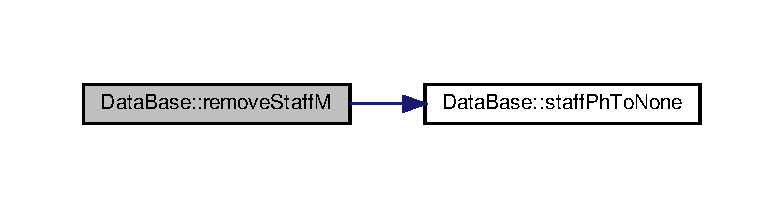
\includegraphics[width=350pt]{classDataBase_a79dbf45f9b1a60fd5a29505f44e188e0_cgraph}
\end{center}
\end{figure}
\mbox{\Hypertarget{classDataBase_a26ab8f3d2cb6d78a5105e72c2377c21c}\label{classDataBase_a26ab8f3d2cb6d78a5105e72c2377c21c}} 
\index{Data\+Base@{Data\+Base}!remove\+Staff\+Member@{remove\+Staff\+Member}}
\index{remove\+Staff\+Member@{remove\+Staff\+Member}!Data\+Base@{Data\+Base}}
\subsubsection{\texorpdfstring{remove\+Staff\+Member()}{removeStaffMember()}}
{\footnotesize\ttfamily void Data\+Base\+::remove\+Staff\+Member (\begin{DoxyParamCaption}{ }\end{DoxyParamCaption})}

Here is the call graph for this function\+:\nopagebreak
\begin{figure}[H]
\begin{center}
\leavevmode
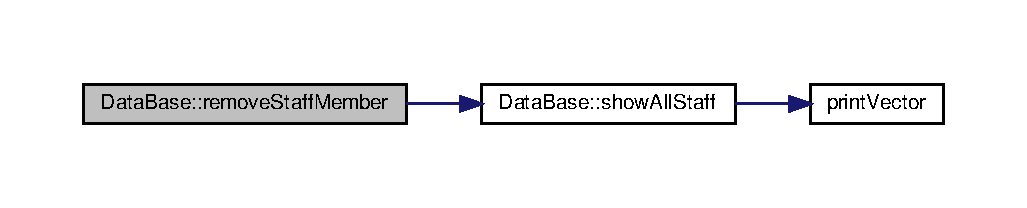
\includegraphics[width=350pt]{classDataBase_a26ab8f3d2cb6d78a5105e72c2377c21c_cgraph}
\end{center}
\end{figure}
\mbox{\Hypertarget{classDataBase_af4762294e1b25415f7de88f0e8d6d90f}\label{classDataBase_af4762294e1b25415f7de88f0e8d6d90f}} 
\index{Data\+Base@{Data\+Base}!show\+All\+Clients@{show\+All\+Clients}}
\index{show\+All\+Clients@{show\+All\+Clients}!Data\+Base@{Data\+Base}}
\subsubsection{\texorpdfstring{show\+All\+Clients()}{showAllClients()}}
{\footnotesize\ttfamily void Data\+Base\+::show\+All\+Clients (\begin{DoxyParamCaption}{ }\end{DoxyParamCaption})}

Here is the call graph for this function\+:\nopagebreak
\begin{figure}[H]
\begin{center}
\leavevmode
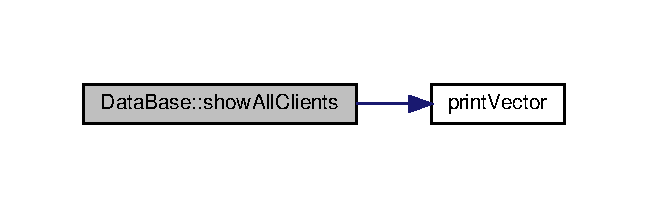
\includegraphics[width=311pt]{classDataBase_af4762294e1b25415f7de88f0e8d6d90f_cgraph}
\end{center}
\end{figure}
\mbox{\Hypertarget{classDataBase_a0c83992321a456f8fa097ea5bbf4a093}\label{classDataBase_a0c83992321a456f8fa097ea5bbf4a093}} 
\index{Data\+Base@{Data\+Base}!show\+All\+ClientsA@{show\+All\+ClientsA}}
\index{show\+All\+ClientsA@{show\+All\+ClientsA}!Data\+Base@{Data\+Base}}
\subsubsection{\texorpdfstring{show\+All\+Clients\+A()}{showAllClientsA()}}
{\footnotesize\ttfamily void Data\+Base\+::show\+All\+ClientsA (\begin{DoxyParamCaption}{ }\end{DoxyParamCaption})}



Displays all the clients in the \hyperlink{classDataBase}{Data\+Base}. 

Here is the call graph for this function\+:\nopagebreak
\begin{figure}[H]
\begin{center}
\leavevmode
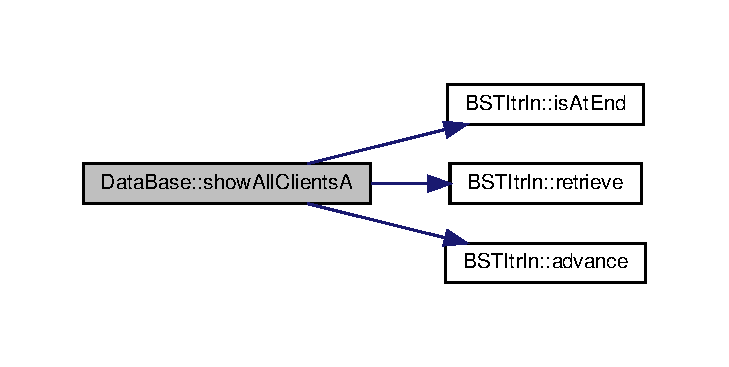
\includegraphics[width=350pt]{classDataBase_a0c83992321a456f8fa097ea5bbf4a093_cgraph}
\end{center}
\end{figure}
\mbox{\Hypertarget{classDataBase_ab00290f55389cd62d8ee5594ecf9a6b5}\label{classDataBase_ab00290f55389cd62d8ee5594ecf9a6b5}} 
\index{Data\+Base@{Data\+Base}!show\+All\+Pharmacies@{show\+All\+Pharmacies}}
\index{show\+All\+Pharmacies@{show\+All\+Pharmacies}!Data\+Base@{Data\+Base}}
\subsubsection{\texorpdfstring{show\+All\+Pharmacies()}{showAllPharmacies()}}
{\footnotesize\ttfamily void Data\+Base\+::show\+All\+Pharmacies (\begin{DoxyParamCaption}{ }\end{DoxyParamCaption})}

Here is the call graph for this function\+:\nopagebreak
\begin{figure}[H]
\begin{center}
\leavevmode
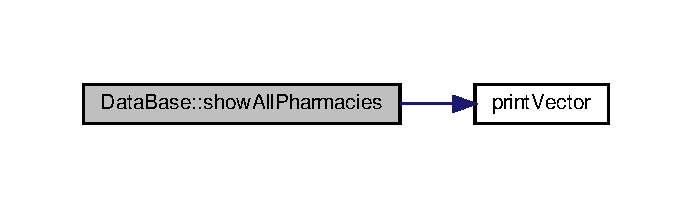
\includegraphics[width=332pt]{classDataBase_ab00290f55389cd62d8ee5594ecf9a6b5_cgraph}
\end{center}
\end{figure}
\mbox{\Hypertarget{classDataBase_a40a951f6f2c923ca315655956ab8e196}\label{classDataBase_a40a951f6f2c923ca315655956ab8e196}} 
\index{Data\+Base@{Data\+Base}!show\+All\+Prescriptions@{show\+All\+Prescriptions}}
\index{show\+All\+Prescriptions@{show\+All\+Prescriptions}!Data\+Base@{Data\+Base}}
\subsubsection{\texorpdfstring{show\+All\+Prescriptions()}{showAllPrescriptions()}}
{\footnotesize\ttfamily void Data\+Base\+::show\+All\+Prescriptions (\begin{DoxyParamCaption}{ }\end{DoxyParamCaption})}

Here is the call graph for this function\+:\nopagebreak
\begin{figure}[H]
\begin{center}
\leavevmode
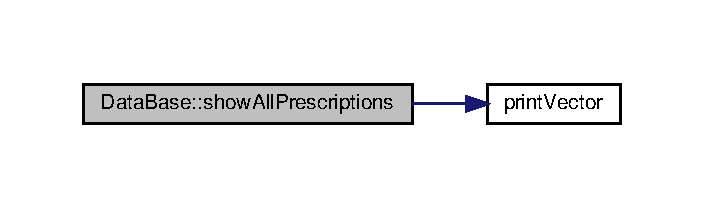
\includegraphics[width=338pt]{classDataBase_a40a951f6f2c923ca315655956ab8e196_cgraph}
\end{center}
\end{figure}
\mbox{\Hypertarget{classDataBase_a74dcc435917c328bd89aaf5fd3cb804d}\label{classDataBase_a74dcc435917c328bd89aaf5fd3cb804d}} 
\index{Data\+Base@{Data\+Base}!show\+All\+Products@{show\+All\+Products}}
\index{show\+All\+Products@{show\+All\+Products}!Data\+Base@{Data\+Base}}
\subsubsection{\texorpdfstring{show\+All\+Products()}{showAllProducts()}}
{\footnotesize\ttfamily void Data\+Base\+::show\+All\+Products (\begin{DoxyParamCaption}{ }\end{DoxyParamCaption})}

\mbox{\Hypertarget{classDataBase_abf8a64bd81ce3207862b0105d52f646f}\label{classDataBase_abf8a64bd81ce3207862b0105d52f646f}} 
\index{Data\+Base@{Data\+Base}!show\+All\+Sales@{show\+All\+Sales}}
\index{show\+All\+Sales@{show\+All\+Sales}!Data\+Base@{Data\+Base}}
\subsubsection{\texorpdfstring{show\+All\+Sales()}{showAllSales()}}
{\footnotesize\ttfamily void Data\+Base\+::show\+All\+Sales (\begin{DoxyParamCaption}{ }\end{DoxyParamCaption})}

Here is the call graph for this function\+:\nopagebreak
\begin{figure}[H]
\begin{center}
\leavevmode
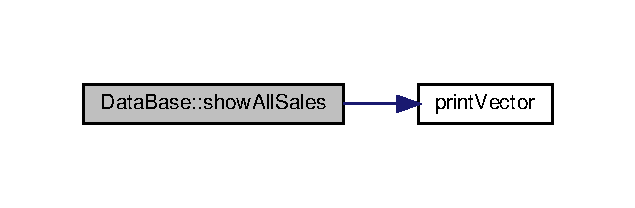
\includegraphics[width=305pt]{classDataBase_abf8a64bd81ce3207862b0105d52f646f_cgraph}
\end{center}
\end{figure}
\mbox{\Hypertarget{classDataBase_aa1d2ae05f581ec45eb8da06e468aec30}\label{classDataBase_aa1d2ae05f581ec45eb8da06e468aec30}} 
\index{Data\+Base@{Data\+Base}!show\+All\+Staff@{show\+All\+Staff}}
\index{show\+All\+Staff@{show\+All\+Staff}!Data\+Base@{Data\+Base}}
\subsubsection{\texorpdfstring{show\+All\+Staff()}{showAllStaff()}}
{\footnotesize\ttfamily void Data\+Base\+::show\+All\+Staff (\begin{DoxyParamCaption}{ }\end{DoxyParamCaption})}

Here is the call graph for this function\+:\nopagebreak
\begin{figure}[H]
\begin{center}
\leavevmode
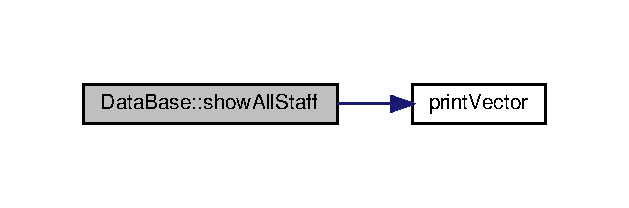
\includegraphics[width=302pt]{classDataBase_aa1d2ae05f581ec45eb8da06e468aec30_cgraph}
\end{center}
\end{figure}
\mbox{\Hypertarget{classDataBase_a2016794a78b86df19676ea9aba3114bc}\label{classDataBase_a2016794a78b86df19676ea9aba3114bc}} 
\index{Data\+Base@{Data\+Base}!show\+Clients\+By\+District@{show\+Clients\+By\+District}}
\index{show\+Clients\+By\+District@{show\+Clients\+By\+District}!Data\+Base@{Data\+Base}}
\subsubsection{\texorpdfstring{show\+Clients\+By\+District()}{showClientsByDistrict()}}
{\footnotesize\ttfamily void Data\+Base\+::show\+Clients\+By\+District (\begin{DoxyParamCaption}{ }\end{DoxyParamCaption})}



Displays all clients from a specific district. 


\begin{DoxyParams}{Parameters}
{\em district} & Name of the district we want to show the clients from \\
\hline
\end{DoxyParams}
Here is the call graph for this function\+:\nopagebreak
\begin{figure}[H]
\begin{center}
\leavevmode
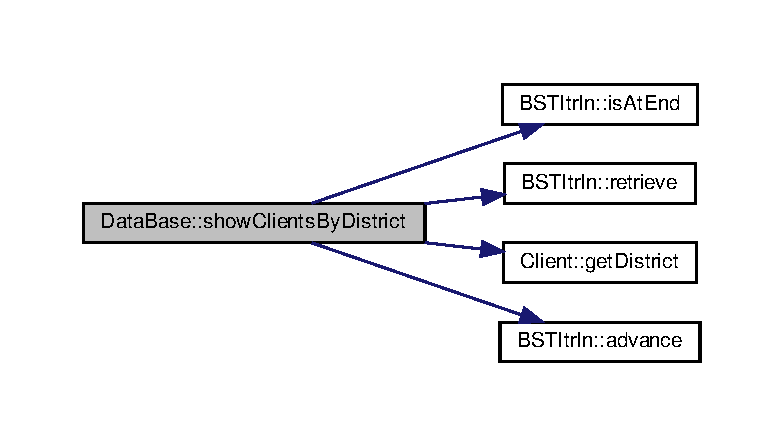
\includegraphics[width=350pt]{classDataBase_a2016794a78b86df19676ea9aba3114bc_cgraph}
\end{center}
\end{figure}
\mbox{\Hypertarget{classDataBase_ab87e9a50f26c934790774b0bf0d62a51}\label{classDataBase_ab87e9a50f26c934790774b0bf0d62a51}} 
\index{Data\+Base@{Data\+Base}!show\+Clients\+With\+Most\+Purchases@{show\+Clients\+With\+Most\+Purchases}}
\index{show\+Clients\+With\+Most\+Purchases@{show\+Clients\+With\+Most\+Purchases}!Data\+Base@{Data\+Base}}
\subsubsection{\texorpdfstring{show\+Clients\+With\+Most\+Purchases()}{showClientsWithMostPurchases()}}
{\footnotesize\ttfamily void Data\+Base\+::show\+Clients\+With\+Most\+Purchases (\begin{DoxyParamCaption}{ }\end{DoxyParamCaption})}



Displays the clients on the top 3 of most purchases made. 

Here is the call graph for this function\+:\nopagebreak
\begin{figure}[H]
\begin{center}
\leavevmode
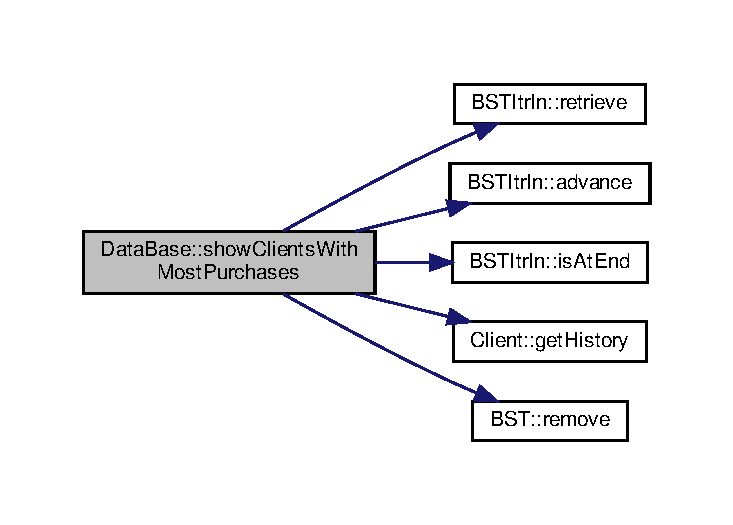
\includegraphics[width=350pt]{classDataBase_ab87e9a50f26c934790774b0bf0d62a51_cgraph}
\end{center}
\end{figure}
\mbox{\Hypertarget{classDataBase_ac572ac9a3091e0adcef16ab79bfba7fb}\label{classDataBase_ac572ac9a3091e0adcef16ab79bfba7fb}} 
\index{Data\+Base@{Data\+Base}!show\+Pharmacies\+Names@{show\+Pharmacies\+Names}}
\index{show\+Pharmacies\+Names@{show\+Pharmacies\+Names}!Data\+Base@{Data\+Base}}
\subsubsection{\texorpdfstring{show\+Pharmacies\+Names()}{showPharmaciesNames()}}
{\footnotesize\ttfamily void Data\+Base\+::show\+Pharmacies\+Names (\begin{DoxyParamCaption}{ }\end{DoxyParamCaption})}



Displays the names of the pharmacies available in the DB. 

\mbox{\Hypertarget{classDataBase_ab17fba12d1810b3548615b3ac0427850}\label{classDataBase_ab17fba12d1810b3548615b3ac0427850}} 
\index{Data\+Base@{Data\+Base}!show\+Staff\+Without\+Ph@{show\+Staff\+Without\+Ph}}
\index{show\+Staff\+Without\+Ph@{show\+Staff\+Without\+Ph}!Data\+Base@{Data\+Base}}
\subsubsection{\texorpdfstring{show\+Staff\+Without\+Ph()}{showStaffWithoutPh()}}
{\footnotesize\ttfamily void Data\+Base\+::show\+Staff\+Without\+Ph (\begin{DoxyParamCaption}{ }\end{DoxyParamCaption})}



Displays all \hyperlink{classStaffMember}{Staff\+Member} \textquotesingle{}s in the \hyperlink{classDataBase}{Data\+Base} with no \hyperlink{classPharmacy}{Pharmacy} assigned. 

\mbox{\Hypertarget{classDataBase_a85445c22323399e318780faf36854c2f}\label{classDataBase_a85445c22323399e318780faf36854c2f}} 
\index{Data\+Base@{Data\+Base}!staff\+Ph\+To\+None@{staff\+Ph\+To\+None}}
\index{staff\+Ph\+To\+None@{staff\+Ph\+To\+None}!Data\+Base@{Data\+Base}}
\subsubsection{\texorpdfstring{staff\+Ph\+To\+None()}{staffPhToNone()}}
{\footnotesize\ttfamily void Data\+Base\+::staff\+Ph\+To\+None (\begin{DoxyParamCaption}\item[{string}]{name }\end{DoxyParamCaption})}

\mbox{\Hypertarget{classDataBase_a4d855ccf967f4f741646100d2c890ede}\label{classDataBase_a4d855ccf967f4f741646100d2c890ede}} 
\index{Data\+Base@{Data\+Base}!write\+To\+Clients\+File@{write\+To\+Clients\+File}}
\index{write\+To\+Clients\+File@{write\+To\+Clients\+File}!Data\+Base@{Data\+Base}}
\subsubsection{\texorpdfstring{write\+To\+Clients\+File()}{writeToClientsFile()}}
{\footnotesize\ttfamily void Data\+Base\+::write\+To\+Clients\+File (\begin{DoxyParamCaption}{ }\end{DoxyParamCaption})}

Here is the call graph for this function\+:\nopagebreak
\begin{figure}[H]
\begin{center}
\leavevmode
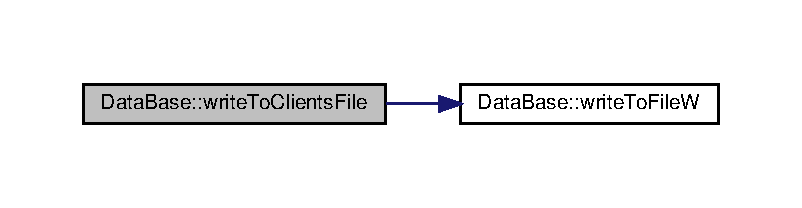
\includegraphics[width=350pt]{classDataBase_a4d855ccf967f4f741646100d2c890ede_cgraph}
\end{center}
\end{figure}
\mbox{\Hypertarget{classDataBase_a136d789db1f6c1cd615dc1bdbe27557b}\label{classDataBase_a136d789db1f6c1cd615dc1bdbe27557b}} 
\index{Data\+Base@{Data\+Base}!write\+To\+FileW@{write\+To\+FileW}}
\index{write\+To\+FileW@{write\+To\+FileW}!Data\+Base@{Data\+Base}}
\subsubsection{\texorpdfstring{write\+To\+File\+W()}{writeToFileW()}}
{\footnotesize\ttfamily template$<$class T $>$ \\
void Data\+Base\+::write\+To\+FileW (\begin{DoxyParamCaption}\item[{string}]{file\+Name,  }\item[{vector$<$ T $>$}]{v }\end{DoxyParamCaption})\hspace{0.3cm}{\ttfamily [inline]}}

\mbox{\Hypertarget{classDataBase_aef0dc00d9d40159c361518e60e78f857}\label{classDataBase_aef0dc00d9d40159c361518e60e78f857}} 
\index{Data\+Base@{Data\+Base}!write\+To\+Pharmacies\+File@{write\+To\+Pharmacies\+File}}
\index{write\+To\+Pharmacies\+File@{write\+To\+Pharmacies\+File}!Data\+Base@{Data\+Base}}
\subsubsection{\texorpdfstring{write\+To\+Pharmacies\+File()}{writeToPharmaciesFile()}}
{\footnotesize\ttfamily void Data\+Base\+::write\+To\+Pharmacies\+File (\begin{DoxyParamCaption}{ }\end{DoxyParamCaption})}

Here is the call graph for this function\+:\nopagebreak
\begin{figure}[H]
\begin{center}
\leavevmode
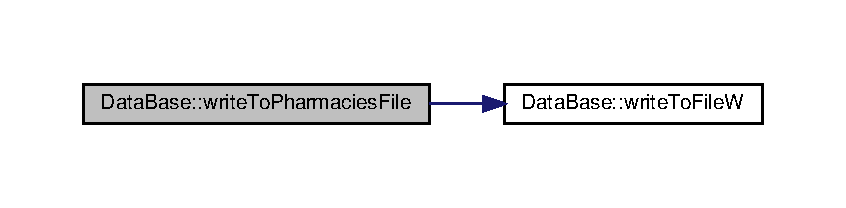
\includegraphics[width=350pt]{classDataBase_aef0dc00d9d40159c361518e60e78f857_cgraph}
\end{center}
\end{figure}
\mbox{\Hypertarget{classDataBase_a1435e1728598586503f199981b84a933}\label{classDataBase_a1435e1728598586503f199981b84a933}} 
\index{Data\+Base@{Data\+Base}!write\+To\+Prescription\+File@{write\+To\+Prescription\+File}}
\index{write\+To\+Prescription\+File@{write\+To\+Prescription\+File}!Data\+Base@{Data\+Base}}
\subsubsection{\texorpdfstring{write\+To\+Prescription\+File()}{writeToPrescriptionFile()}}
{\footnotesize\ttfamily void Data\+Base\+::write\+To\+Prescription\+File (\begin{DoxyParamCaption}{ }\end{DoxyParamCaption})}

Here is the call graph for this function\+:\nopagebreak
\begin{figure}[H]
\begin{center}
\leavevmode
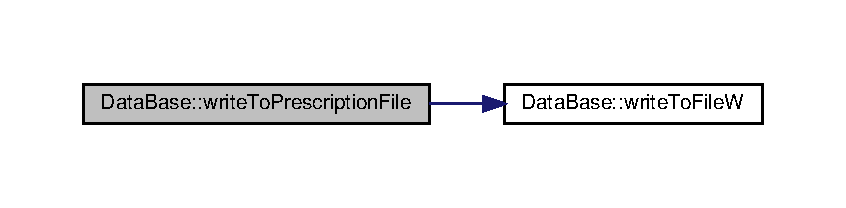
\includegraphics[width=350pt]{classDataBase_a1435e1728598586503f199981b84a933_cgraph}
\end{center}
\end{figure}
\mbox{\Hypertarget{classDataBase_a108ba0eb315d14ed6bc7181b98499318}\label{classDataBase_a108ba0eb315d14ed6bc7181b98499318}} 
\index{Data\+Base@{Data\+Base}!write\+To\+Products\+File@{write\+To\+Products\+File}}
\index{write\+To\+Products\+File@{write\+To\+Products\+File}!Data\+Base@{Data\+Base}}
\subsubsection{\texorpdfstring{write\+To\+Products\+File()}{writeToProductsFile()}}
{\footnotesize\ttfamily void Data\+Base\+::write\+To\+Products\+File (\begin{DoxyParamCaption}{ }\end{DoxyParamCaption})}

Here is the call graph for this function\+:\nopagebreak
\begin{figure}[H]
\begin{center}
\leavevmode
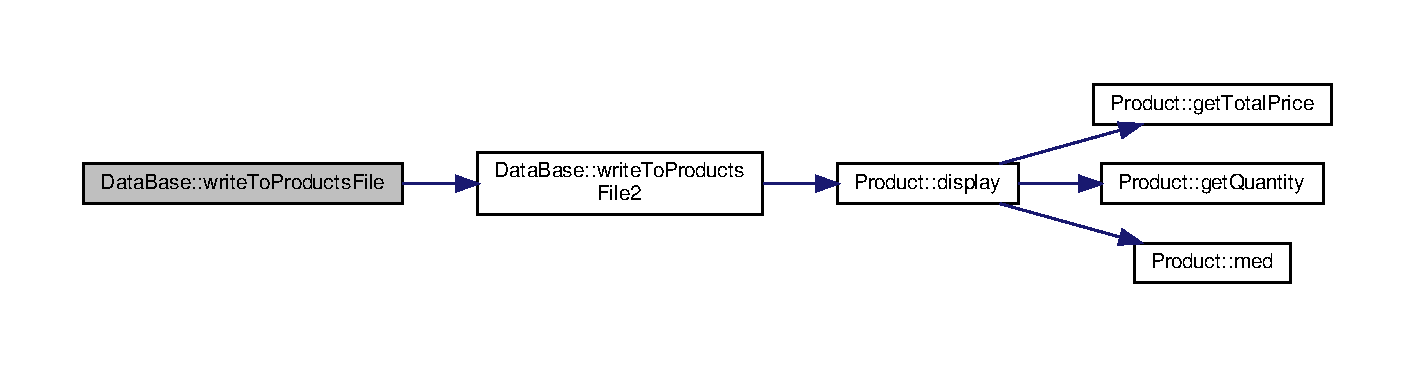
\includegraphics[width=350pt]{classDataBase_a108ba0eb315d14ed6bc7181b98499318_cgraph}
\end{center}
\end{figure}
\mbox{\Hypertarget{classDataBase_aec542d0eb4b2c2d44abe5cefd25d2057}\label{classDataBase_aec542d0eb4b2c2d44abe5cefd25d2057}} 
\index{Data\+Base@{Data\+Base}!write\+To\+Products\+File2@{write\+To\+Products\+File2}}
\index{write\+To\+Products\+File2@{write\+To\+Products\+File2}!Data\+Base@{Data\+Base}}
\subsubsection{\texorpdfstring{write\+To\+Products\+File2()}{writeToProductsFile2()}}
{\footnotesize\ttfamily void Data\+Base\+::write\+To\+Products\+File2 (\begin{DoxyParamCaption}\item[{string}]{file\+Name }\end{DoxyParamCaption})\hspace{0.3cm}{\ttfamily [inline]}}

Here is the call graph for this function\+:\nopagebreak
\begin{figure}[H]
\begin{center}
\leavevmode
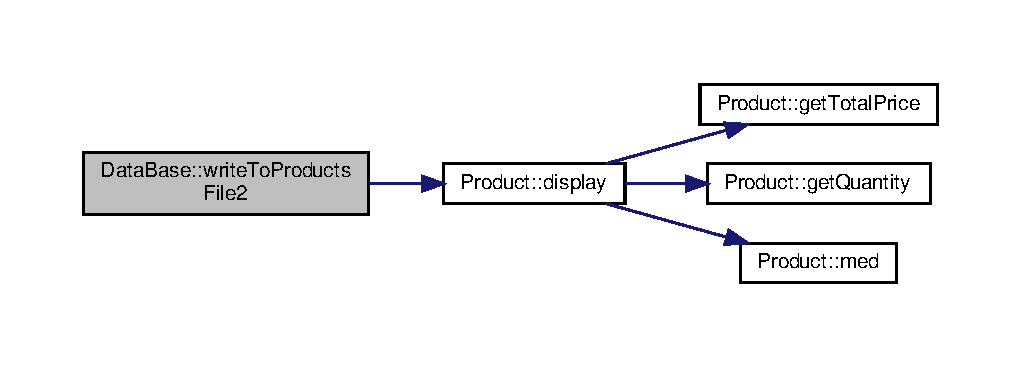
\includegraphics[width=350pt]{classDataBase_aec542d0eb4b2c2d44abe5cefd25d2057_cgraph}
\end{center}
\end{figure}
\mbox{\Hypertarget{classDataBase_a0bf85b7fb0feb4fb1f6888ba58ebe2b2}\label{classDataBase_a0bf85b7fb0feb4fb1f6888ba58ebe2b2}} 
\index{Data\+Base@{Data\+Base}!write\+To\+Sales@{write\+To\+Sales}}
\index{write\+To\+Sales@{write\+To\+Sales}!Data\+Base@{Data\+Base}}
\subsubsection{\texorpdfstring{write\+To\+Sales()}{writeToSales()}}
{\footnotesize\ttfamily void Data\+Base\+::write\+To\+Sales (\begin{DoxyParamCaption}\item[{string}]{file\+Name }\end{DoxyParamCaption})\hspace{0.3cm}{\ttfamily [inline]}}



Writes the info saved in the \hyperlink{classDataBase}{Data\+Base} to the Sales file. 


\begin{DoxyParams}{Parameters}
{\em file\+Name} & Name of the file to be written to \\
\hline
\end{DoxyParams}
\mbox{\Hypertarget{classDataBase_a62cb54f7bbcd213d71f604003298cd95}\label{classDataBase_a62cb54f7bbcd213d71f604003298cd95}} 
\index{Data\+Base@{Data\+Base}!write\+To\+Sales\+File@{write\+To\+Sales\+File}}
\index{write\+To\+Sales\+File@{write\+To\+Sales\+File}!Data\+Base@{Data\+Base}}
\subsubsection{\texorpdfstring{write\+To\+Sales\+File()}{writeToSalesFile()}}
{\footnotesize\ttfamily void Data\+Base\+::write\+To\+Sales\+File (\begin{DoxyParamCaption}{ }\end{DoxyParamCaption})}

Here is the call graph for this function\+:\nopagebreak
\begin{figure}[H]
\begin{center}
\leavevmode
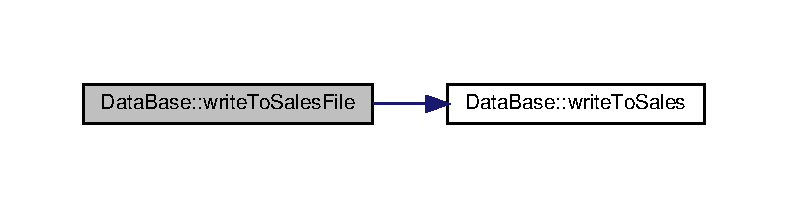
\includegraphics[width=350pt]{classDataBase_a62cb54f7bbcd213d71f604003298cd95_cgraph}
\end{center}
\end{figure}
\mbox{\Hypertarget{classDataBase_abc8c8d3116c6b3422d87ae781ba91538}\label{classDataBase_abc8c8d3116c6b3422d87ae781ba91538}} 
\index{Data\+Base@{Data\+Base}!write\+To\+Staff\+File@{write\+To\+Staff\+File}}
\index{write\+To\+Staff\+File@{write\+To\+Staff\+File}!Data\+Base@{Data\+Base}}
\subsubsection{\texorpdfstring{write\+To\+Staff\+File()}{writeToStaffFile()}}
{\footnotesize\ttfamily void Data\+Base\+::write\+To\+Staff\+File (\begin{DoxyParamCaption}{ }\end{DoxyParamCaption})}

Here is the call graph for this function\+:\nopagebreak
\begin{figure}[H]
\begin{center}
\leavevmode
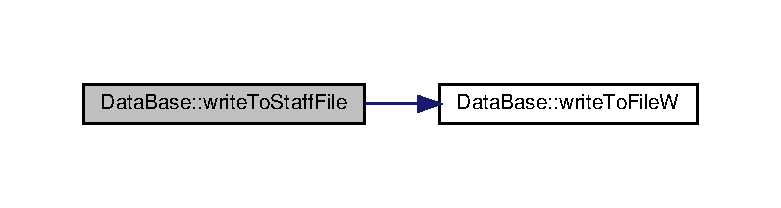
\includegraphics[width=350pt]{classDataBase_abc8c8d3116c6b3422d87ae781ba91538_cgraph}
\end{center}
\end{figure}


\subsection{Member Data Documentation}
\mbox{\Hypertarget{classDataBase_aa5f93e5229c216c200681b551db2db77}\label{classDataBase_aa5f93e5229c216c200681b551db2db77}} 
\index{Data\+Base@{Data\+Base}!clients@{clients}}
\index{clients@{clients}!Data\+Base@{Data\+Base}}
\subsubsection{\texorpdfstring{clients}{clients}}
{\footnotesize\ttfamily vector$<$\hyperlink{classClient}{Client}$>$ Data\+Base\+::clients\hspace{0.3cm}{\ttfamily [private]}}

\mbox{\Hypertarget{classDataBase_a9b3973c4282ee24f7769f4f735b4b898}\label{classDataBase_a9b3973c4282ee24f7769f4f735b4b898}} 
\index{Data\+Base@{Data\+Base}!clientsA@{clientsA}}
\index{clientsA@{clientsA}!Data\+Base@{Data\+Base}}
\subsubsection{\texorpdfstring{clientsA}{clientsA}}
{\footnotesize\ttfamily \hyperlink{classBST}{B\+ST}$<$\hyperlink{classClient}{Client}$>$ Data\+Base\+::clientsA\hspace{0.3cm}{\ttfamily [private]}}



vector for sales 

\mbox{\Hypertarget{classDataBase_a7b52741a2183b8b3eba86534d02782e6}\label{classDataBase_a7b52741a2183b8b3eba86534d02782e6}} 
\index{Data\+Base@{Data\+Base}!clients\+File@{clients\+File}}
\index{clients\+File@{clients\+File}!Data\+Base@{Data\+Base}}
\subsubsection{\texorpdfstring{clients\+File}{clientsFile}}
{\footnotesize\ttfamily string Data\+Base\+::clients\+File\hspace{0.3cm}{\ttfamily [private]}}

\mbox{\Hypertarget{classDataBase_a576f0eac012d39fffb1064a5ea27ad08}\label{classDataBase_a576f0eac012d39fffb1064a5ea27ad08}} 
\index{Data\+Base@{Data\+Base}!files@{files}}
\index{files@{files}!Data\+Base@{Data\+Base}}
\subsubsection{\texorpdfstring{files}{files}}
{\footnotesize\ttfamily \hyperlink{DataBase_8h_a309f0ca910338932f751c46c6e5ccbbc}{files\+HT} Data\+Base\+::files\hspace{0.3cm}{\ttfamily [private]}}



files names 

\mbox{\Hypertarget{classDataBase_ada5f113e22144b1b28775557e2a10f08}\label{classDataBase_ada5f113e22144b1b28775557e2a10f08}} 
\index{Data\+Base@{Data\+Base}!pharmacies@{pharmacies}}
\index{pharmacies@{pharmacies}!Data\+Base@{Data\+Base}}
\subsubsection{\texorpdfstring{pharmacies}{pharmacies}}
{\footnotesize\ttfamily vector$<$\hyperlink{classPharmacy}{Pharmacy}$>$ Data\+Base\+::pharmacies\hspace{0.3cm}{\ttfamily [private]}}



vector for clients 

\mbox{\Hypertarget{classDataBase_aa52765a56e1fefddb5b1cf638de3493e}\label{classDataBase_aa52765a56e1fefddb5b1cf638de3493e}} 
\index{Data\+Base@{Data\+Base}!pharmacies\+File@{pharmacies\+File}}
\index{pharmacies\+File@{pharmacies\+File}!Data\+Base@{Data\+Base}}
\subsubsection{\texorpdfstring{pharmacies\+File}{pharmaciesFile}}
{\footnotesize\ttfamily string Data\+Base\+::pharmacies\+File\hspace{0.3cm}{\ttfamily [private]}}

\mbox{\Hypertarget{classDataBase_a7649e7e3eda974285c99e78c23829334}\label{classDataBase_a7649e7e3eda974285c99e78c23829334}} 
\index{Data\+Base@{Data\+Base}!presc\+File@{presc\+File}}
\index{presc\+File@{presc\+File}!Data\+Base@{Data\+Base}}
\subsubsection{\texorpdfstring{presc\+File}{prescFile}}
{\footnotesize\ttfamily string Data\+Base\+::presc\+File\hspace{0.3cm}{\ttfamily [private]}}

\mbox{\Hypertarget{classDataBase_a592b7e885d6708309c298406db68c505}\label{classDataBase_a592b7e885d6708309c298406db68c505}} 
\index{Data\+Base@{Data\+Base}!prescriptions@{prescriptions}}
\index{prescriptions@{prescriptions}!Data\+Base@{Data\+Base}}
\subsubsection{\texorpdfstring{prescriptions}{prescriptions}}
{\footnotesize\ttfamily vector$<$\hyperlink{classPrescription}{Prescription}$>$ Data\+Base\+::prescriptions\hspace{0.3cm}{\ttfamily [private]}}



vector for staff 

\mbox{\Hypertarget{classDataBase_a83dd84eb12b869e3e585fe965c414eef}\label{classDataBase_a83dd84eb12b869e3e585fe965c414eef}} 
\index{Data\+Base@{Data\+Base}!products@{products}}
\index{products@{products}!Data\+Base@{Data\+Base}}
\subsubsection{\texorpdfstring{products}{products}}
{\footnotesize\ttfamily priority\+\_\+queue$<$\hyperlink{classProduct}{Product}$>$ Data\+Base\+::products\hspace{0.3cm}{\ttfamily [private]}}



\hyperlink{classBST}{B\+ST} for the clients. 

\mbox{\Hypertarget{classDataBase_a24acb8bdda9293336f40a4b08741235e}\label{classDataBase_a24acb8bdda9293336f40a4b08741235e}} 
\index{Data\+Base@{Data\+Base}!products\+File@{products\+File}}
\index{products\+File@{products\+File}!Data\+Base@{Data\+Base}}
\subsubsection{\texorpdfstring{products\+File}{productsFile}}
{\footnotesize\ttfamily string Data\+Base\+::products\+File\hspace{0.3cm}{\ttfamily [private]}}

\mbox{\Hypertarget{classDataBase_a4e48e9c0e840c7f9febf3344c5a003ba}\label{classDataBase_a4e48e9c0e840c7f9febf3344c5a003ba}} 
\index{Data\+Base@{Data\+Base}!sales@{sales}}
\index{sales@{sales}!Data\+Base@{Data\+Base}}
\subsubsection{\texorpdfstring{sales}{sales}}
{\footnotesize\ttfamily vector$<$\hyperlink{classSale}{Sale}$>$ Data\+Base\+::sales\hspace{0.3cm}{\ttfamily [private]}}



vector for prescriptions 

\mbox{\Hypertarget{classDataBase_a8b16f4814de788f12e96163255aaa737}\label{classDataBase_a8b16f4814de788f12e96163255aaa737}} 
\index{Data\+Base@{Data\+Base}!sales\+File@{sales\+File}}
\index{sales\+File@{sales\+File}!Data\+Base@{Data\+Base}}
\subsubsection{\texorpdfstring{sales\+File}{salesFile}}
{\footnotesize\ttfamily string Data\+Base\+::sales\+File\hspace{0.3cm}{\ttfamily [private]}}

\mbox{\Hypertarget{classDataBase_a74729cf98d5b60cc2bfbac6c0fa00229}\label{classDataBase_a74729cf98d5b60cc2bfbac6c0fa00229}} 
\index{Data\+Base@{Data\+Base}!staff@{staff}}
\index{staff@{staff}!Data\+Base@{Data\+Base}}
\subsubsection{\texorpdfstring{staff}{staff}}
{\footnotesize\ttfamily vector$<$\hyperlink{classStaffMember}{Staff\+Member}$>$ Data\+Base\+::staff\hspace{0.3cm}{\ttfamily [private]}}



vector for pharmacies 

\mbox{\Hypertarget{classDataBase_a2f564a52132d74186314695a7a0e3270}\label{classDataBase_a2f564a52132d74186314695a7a0e3270}} 
\index{Data\+Base@{Data\+Base}!staff\+File@{staff\+File}}
\index{staff\+File@{staff\+File}!Data\+Base@{Data\+Base}}
\subsubsection{\texorpdfstring{staff\+File}{staffFile}}
{\footnotesize\ttfamily string Data\+Base\+::staff\+File\hspace{0.3cm}{\ttfamily [private]}}



The documentation for this class was generated from the following files\+:\begin{DoxyCompactItemize}
\item 
src/\hyperlink{DataBase_8h}{Data\+Base.\+h}\item 
src/\hyperlink{DataBase_8cpp}{Data\+Base.\+cpp}\end{DoxyCompactItemize}

\hypertarget{classEntity}{}\section{Entity Class Reference}
\label{classEntity}\index{Entity@{Entity}}


\hyperlink{classEntity}{Entity} Class that represents a entity(can be a Person or a Pharmacy) where are stored the name and address.  




{\ttfamily \#include $<$Entity.\+h$>$}



Inheritance diagram for Entity\+:
\nopagebreak
\begin{figure}[H]
\begin{center}
\leavevmode
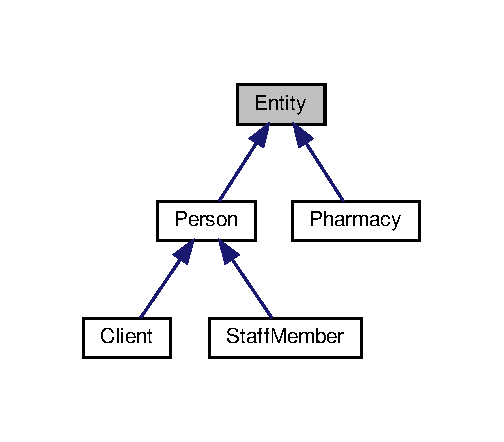
\includegraphics[width=242pt]{classEntity__inherit__graph}
\end{center}
\end{figure}
\subsection*{Public Member Functions}
\begin{DoxyCompactItemize}
\item 
\hyperlink{classEntity_ae540a46bdc1983a49127e0ac31884eee}{Entity} (string n, string addr)
\begin{DoxyCompactList}\small\item\em address of the \hyperlink{classEntity}{Entity} \end{DoxyCompactList}\item 
string \hyperlink{classEntity_a438837d2be5b221fd9aafc323c46f08a}{get\+Name} () const
\begin{DoxyCompactList}\small\item\em Get the Name object. \end{DoxyCompactList}\item 
string \hyperlink{classEntity_a8acaa5f9e84722ea668a0e33789c347e}{get\+Address} () const
\begin{DoxyCompactList}\small\item\em Get the Address object. \end{DoxyCompactList}\item 
void \hyperlink{classEntity_a6b6078942e4000e136e13aeccefba0eb}{set\+Name} (string nn)
\begin{DoxyCompactList}\small\item\em Set the Name object. \end{DoxyCompactList}\item 
void \hyperlink{classEntity_ae362658ba037f024aa5edc2cdce2d833}{set\+Address} (string naddr)
\begin{DoxyCompactList}\small\item\em Set the Address object. \end{DoxyCompactList}\end{DoxyCompactItemize}
\subsection*{Private Attributes}
\begin{DoxyCompactItemize}
\item 
string \hyperlink{classEntity_afb45718695f537c330a463168616c262}{name}
\item 
string \hyperlink{classEntity_a3db10b65d221e6066fbdeebe17d5af42}{address}
\begin{DoxyCompactList}\small\item\em name of the \hyperlink{classEntity}{Entity} \end{DoxyCompactList}\end{DoxyCompactItemize}
\subsection*{Friends}
\begin{DoxyCompactItemize}
\item 
ostream \& \hyperlink{classEntity_a985385a6f8478ba830ea909fc233c150}{operator$<$$<$} (ostream \&os, const \hyperlink{classEntity}{Entity} \&e)
\begin{DoxyCompactList}\small\item\em Overload outstream operator $<$$<$ to write an \hyperlink{classEntity}{Entity} to an Oustream. \end{DoxyCompactList}\end{DoxyCompactItemize}


\subsection{Detailed Description}
\hyperlink{classEntity}{Entity} Class that represents a entity(can be a Person or a Pharmacy) where are stored the name and address. 

\subsection{Constructor \& Destructor Documentation}
\mbox{\Hypertarget{classEntity_ae540a46bdc1983a49127e0ac31884eee}\label{classEntity_ae540a46bdc1983a49127e0ac31884eee}} 
\index{Entity@{Entity}!Entity@{Entity}}
\index{Entity@{Entity}!Entity@{Entity}}
\subsubsection{\texorpdfstring{Entity()}{Entity()}}
{\footnotesize\ttfamily Entity\+::\+Entity (\begin{DoxyParamCaption}\item[{string}]{n,  }\item[{string}]{addr }\end{DoxyParamCaption})}



address of the \hyperlink{classEntity}{Entity} 

$<$ Construct a new \hyperlink{classEntity}{Entity} object


\begin{DoxyParams}{Parameters}
{\em n} & The name of the \hyperlink{classEntity}{Entity} to be created \\
\hline
{\em addr} & The adress of the \hyperlink{classEntity}{Entity} to be created \\
\hline
\end{DoxyParams}


\subsection{Member Function Documentation}
\mbox{\Hypertarget{classEntity_a8acaa5f9e84722ea668a0e33789c347e}\label{classEntity_a8acaa5f9e84722ea668a0e33789c347e}} 
\index{Entity@{Entity}!get\+Address@{get\+Address}}
\index{get\+Address@{get\+Address}!Entity@{Entity}}
\subsubsection{\texorpdfstring{get\+Address()}{getAddress()}}
{\footnotesize\ttfamily string Entity\+::get\+Address (\begin{DoxyParamCaption}{ }\end{DoxyParamCaption}) const}



Get the Address object. 

\begin{DoxyReturn}{Returns}
string \hyperlink{classEntity}{Entity}\textquotesingle{}s address 
\end{DoxyReturn}
\mbox{\Hypertarget{classEntity_a438837d2be5b221fd9aafc323c46f08a}\label{classEntity_a438837d2be5b221fd9aafc323c46f08a}} 
\index{Entity@{Entity}!get\+Name@{get\+Name}}
\index{get\+Name@{get\+Name}!Entity@{Entity}}
\subsubsection{\texorpdfstring{get\+Name()}{getName()}}
{\footnotesize\ttfamily string Entity\+::get\+Name (\begin{DoxyParamCaption}{ }\end{DoxyParamCaption}) const}



Get the Name object. 

\begin{DoxyReturn}{Returns}
string \hyperlink{classEntity}{Entity}\textquotesingle{}s name 
\end{DoxyReturn}
\mbox{\Hypertarget{classEntity_ae362658ba037f024aa5edc2cdce2d833}\label{classEntity_ae362658ba037f024aa5edc2cdce2d833}} 
\index{Entity@{Entity}!set\+Address@{set\+Address}}
\index{set\+Address@{set\+Address}!Entity@{Entity}}
\subsubsection{\texorpdfstring{set\+Address()}{setAddress()}}
{\footnotesize\ttfamily void Entity\+::set\+Address (\begin{DoxyParamCaption}\item[{string}]{naddr }\end{DoxyParamCaption})}



Set the Address object. 


\begin{DoxyParams}{Parameters}
{\em naddr} & new \hyperlink{classEntity}{Entity}\textquotesingle{}s address \\
\hline
\end{DoxyParams}
\mbox{\Hypertarget{classEntity_a6b6078942e4000e136e13aeccefba0eb}\label{classEntity_a6b6078942e4000e136e13aeccefba0eb}} 
\index{Entity@{Entity}!set\+Name@{set\+Name}}
\index{set\+Name@{set\+Name}!Entity@{Entity}}
\subsubsection{\texorpdfstring{set\+Name()}{setName()}}
{\footnotesize\ttfamily void Entity\+::set\+Name (\begin{DoxyParamCaption}\item[{string}]{nn }\end{DoxyParamCaption})}



Set the Name object. 


\begin{DoxyParams}{Parameters}
{\em nn} & new \hyperlink{classEntity}{Entity}\textquotesingle{}s name \\
\hline
\end{DoxyParams}


\subsection{Friends And Related Function Documentation}
\mbox{\Hypertarget{classEntity_a985385a6f8478ba830ea909fc233c150}\label{classEntity_a985385a6f8478ba830ea909fc233c150}} 
\index{Entity@{Entity}!operator$<$$<$@{operator$<$$<$}}
\index{operator$<$$<$@{operator$<$$<$}!Entity@{Entity}}
\subsubsection{\texorpdfstring{operator$<$$<$}{operator<<}}
{\footnotesize\ttfamily ostream\& operator$<$$<$ (\begin{DoxyParamCaption}\item[{ostream \&}]{os,  }\item[{const \hyperlink{classEntity}{Entity} \&}]{e }\end{DoxyParamCaption})\hspace{0.3cm}{\ttfamily [friend]}}



Overload outstream operator $<$$<$ to write an \hyperlink{classEntity}{Entity} to an Oustream. 


\begin{DoxyParams}{Parameters}
{\em os} & outstream \\
\hline
{\em e} & \hyperlink{classEntity}{Entity} to be written \\
\hline
\end{DoxyParams}
\begin{DoxyReturn}{Returns}
outstream 
\end{DoxyReturn}


\subsection{Member Data Documentation}
\mbox{\Hypertarget{classEntity_a3db10b65d221e6066fbdeebe17d5af42}\label{classEntity_a3db10b65d221e6066fbdeebe17d5af42}} 
\index{Entity@{Entity}!address@{address}}
\index{address@{address}!Entity@{Entity}}
\subsubsection{\texorpdfstring{address}{address}}
{\footnotesize\ttfamily string Entity\+::address\hspace{0.3cm}{\ttfamily [private]}}



name of the \hyperlink{classEntity}{Entity} 

$<$ \mbox{\Hypertarget{classEntity_afb45718695f537c330a463168616c262}\label{classEntity_afb45718695f537c330a463168616c262}} 
\index{Entity@{Entity}!name@{name}}
\index{name@{name}!Entity@{Entity}}
\subsubsection{\texorpdfstring{name}{name}}
{\footnotesize\ttfamily string Entity\+::name\hspace{0.3cm}{\ttfamily [private]}}



The documentation for this class was generated from the following files\+:\begin{DoxyCompactItemize}
\item 
src/\hyperlink{Entity_8h}{Entity.\+h}\item 
src/\hyperlink{Entity_8cpp}{Entity.\+cpp}\end{DoxyCompactItemize}

\hypertarget{classErrorOpeningFile}{}\section{Error\+Opening\+File Class Reference}
\label{classErrorOpeningFile}\index{Error\+Opening\+File@{Error\+Opening\+File}}


Class for error opening file.  




{\ttfamily \#include $<$Data\+Base.\+h$>$}

\subsection*{Public Member Functions}
\begin{DoxyCompactItemize}
\item 
\hyperlink{classErrorOpeningFile_a48508e7fc3c31fa2a4ea5489fde07411}{Error\+Opening\+File} (string name)
\begin{DoxyCompactList}\small\item\em name of File \end{DoxyCompactList}\item 
string \hyperlink{classErrorOpeningFile_a6177800f93b1e928ead4f55ef3421120}{get\+File\+Name} ()
\begin{DoxyCompactList}\small\item\em Gets the file name. \end{DoxyCompactList}\end{DoxyCompactItemize}
\subsection*{Private Attributes}
\begin{DoxyCompactItemize}
\item 
string \hyperlink{classErrorOpeningFile_a24d6690f6660667ef0532b68e3ee7ea9}{name\+File}
\end{DoxyCompactItemize}


\subsection{Detailed Description}
Class for error opening file. 

\subsection{Constructor \& Destructor Documentation}
\mbox{\Hypertarget{classErrorOpeningFile_a48508e7fc3c31fa2a4ea5489fde07411}\label{classErrorOpeningFile_a48508e7fc3c31fa2a4ea5489fde07411}} 
\index{Error\+Opening\+File@{Error\+Opening\+File}!Error\+Opening\+File@{Error\+Opening\+File}}
\index{Error\+Opening\+File@{Error\+Opening\+File}!Error\+Opening\+File@{Error\+Opening\+File}}
\subsubsection{\texorpdfstring{Error\+Opening\+File()}{ErrorOpeningFile()}}
{\footnotesize\ttfamily Error\+Opening\+File\+::\+Error\+Opening\+File (\begin{DoxyParamCaption}\item[{string}]{name }\end{DoxyParamCaption})\hspace{0.3cm}{\ttfamily [inline]}}



name of File 

$<$ Constructs the object.


\begin{DoxyParams}{Parameters}
{\em name} & The name of the file \\
\hline
\end{DoxyParams}


\subsection{Member Function Documentation}
\mbox{\Hypertarget{classErrorOpeningFile_a6177800f93b1e928ead4f55ef3421120}\label{classErrorOpeningFile_a6177800f93b1e928ead4f55ef3421120}} 
\index{Error\+Opening\+File@{Error\+Opening\+File}!get\+File\+Name@{get\+File\+Name}}
\index{get\+File\+Name@{get\+File\+Name}!Error\+Opening\+File@{Error\+Opening\+File}}
\subsubsection{\texorpdfstring{get\+File\+Name()}{getFileName()}}
{\footnotesize\ttfamily string Error\+Opening\+File\+::get\+File\+Name (\begin{DoxyParamCaption}{ }\end{DoxyParamCaption})\hspace{0.3cm}{\ttfamily [inline]}}



Gets the file name. 

\begin{DoxyReturn}{Returns}
The file name. 
\end{DoxyReturn}


\subsection{Member Data Documentation}
\mbox{\Hypertarget{classErrorOpeningFile_a24d6690f6660667ef0532b68e3ee7ea9}\label{classErrorOpeningFile_a24d6690f6660667ef0532b68e3ee7ea9}} 
\index{Error\+Opening\+File@{Error\+Opening\+File}!name\+File@{name\+File}}
\index{name\+File@{name\+File}!Error\+Opening\+File@{Error\+Opening\+File}}
\subsubsection{\texorpdfstring{name\+File}{nameFile}}
{\footnotesize\ttfamily string Error\+Opening\+File\+::name\+File\hspace{0.3cm}{\ttfamily [private]}}



The documentation for this class was generated from the following file\+:\begin{DoxyCompactItemize}
\item 
src/\hyperlink{DataBase_8h}{Data\+Base.\+h}\end{DoxyCompactItemize}

\hypertarget{classItemDoesNotExist}{}\section{Item\+Does\+Not\+Exist Class Reference}
\label{classItemDoesNotExist}\index{Item\+Does\+Not\+Exist@{Item\+Does\+Not\+Exist}}


Class for when an item does not exist.  




{\ttfamily \#include $<$Data\+Base.\+h$>$}

\subsection*{Public Member Functions}
\begin{DoxyCompactItemize}
\item 
\hyperlink{classItemDoesNotExist_aa5e1ee7b9ba756f3f69643ccc956877f}{Item\+Does\+Not\+Exist} (string n)
\begin{DoxyCompactList}\small\item\em item name \end{DoxyCompactList}\item 
void \hyperlink{classItemDoesNotExist_ac043ce235a565e8766cf55b32a2aa80c}{print\+Msg} ()
\end{DoxyCompactItemize}
\subsection*{Private Attributes}
\begin{DoxyCompactItemize}
\item 
string \hyperlink{classItemDoesNotExist_ac1848f31f6668f41a166b4976189ec0f}{item}
\end{DoxyCompactItemize}


\subsection{Detailed Description}
Class for when an item does not exist. 

\subsection{Constructor \& Destructor Documentation}
\mbox{\Hypertarget{classItemDoesNotExist_aa5e1ee7b9ba756f3f69643ccc956877f}\label{classItemDoesNotExist_aa5e1ee7b9ba756f3f69643ccc956877f}} 
\index{Item\+Does\+Not\+Exist@{Item\+Does\+Not\+Exist}!Item\+Does\+Not\+Exist@{Item\+Does\+Not\+Exist}}
\index{Item\+Does\+Not\+Exist@{Item\+Does\+Not\+Exist}!Item\+Does\+Not\+Exist@{Item\+Does\+Not\+Exist}}
\subsubsection{\texorpdfstring{Item\+Does\+Not\+Exist()}{ItemDoesNotExist()}}
{\footnotesize\ttfamily Item\+Does\+Not\+Exist\+::\+Item\+Does\+Not\+Exist (\begin{DoxyParamCaption}\item[{string}]{n }\end{DoxyParamCaption})\hspace{0.3cm}{\ttfamily [inline]}}



item name 

$<$ Constructs the object.


\begin{DoxyParams}{Parameters}
{\em n} & name \\
\hline
\end{DoxyParams}


\subsection{Member Function Documentation}
\mbox{\Hypertarget{classItemDoesNotExist_ac043ce235a565e8766cf55b32a2aa80c}\label{classItemDoesNotExist_ac043ce235a565e8766cf55b32a2aa80c}} 
\index{Item\+Does\+Not\+Exist@{Item\+Does\+Not\+Exist}!print\+Msg@{print\+Msg}}
\index{print\+Msg@{print\+Msg}!Item\+Does\+Not\+Exist@{Item\+Does\+Not\+Exist}}
\subsubsection{\texorpdfstring{print\+Msg()}{printMsg()}}
{\footnotesize\ttfamily void Item\+Does\+Not\+Exist\+::print\+Msg (\begin{DoxyParamCaption}{ }\end{DoxyParamCaption})\hspace{0.3cm}{\ttfamily [inline]}}



\subsection{Member Data Documentation}
\mbox{\Hypertarget{classItemDoesNotExist_ac1848f31f6668f41a166b4976189ec0f}\label{classItemDoesNotExist_ac1848f31f6668f41a166b4976189ec0f}} 
\index{Item\+Does\+Not\+Exist@{Item\+Does\+Not\+Exist}!item@{item}}
\index{item@{item}!Item\+Does\+Not\+Exist@{Item\+Does\+Not\+Exist}}
\subsubsection{\texorpdfstring{item}{item}}
{\footnotesize\ttfamily string Item\+Does\+Not\+Exist\+::item\hspace{0.3cm}{\ttfamily [private]}}



The documentation for this class was generated from the following file\+:\begin{DoxyCompactItemize}
\item 
src/\hyperlink{DataBase_8h}{Data\+Base.\+h}\end{DoxyCompactItemize}

\hypertarget{classMedicine}{}\section{Medicine Class Reference}
\label{classMedicine}\index{Medicine@{Medicine}}


Class for medicine.  




{\ttfamily \#include $<$Medicine.\+h$>$}



Inheritance diagram for Medicine\+:\nopagebreak
\begin{figure}[H]
\begin{center}
\leavevmode
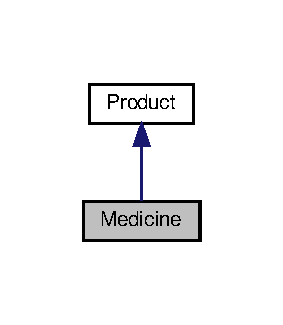
\includegraphics[width=136pt]{classMedicine__inherit__graph}
\end{center}
\end{figure}


Collaboration diagram for Medicine\+:\nopagebreak
\begin{figure}[H]
\begin{center}
\leavevmode
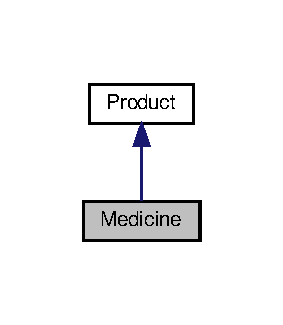
\includegraphics[width=136pt]{classMedicine__coll__graph}
\end{center}
\end{figure}
\subsection*{Public Member Functions}
\begin{DoxyCompactItemize}
\item 
\hyperlink{classMedicine_a6a879be6fb9f5b9b16b465a5aff3f835}{Medicine} ()
\begin{DoxyCompactList}\small\item\em If said \hyperlink{classMedicine}{Medicine} requires a precription. \end{DoxyCompactList}\item 
\hyperlink{classMedicine_a6b66bb37ef10ea4951aa94577f1a1c58}{Medicine} (string \hyperlink{classProduct_acc9bddcf74112d85a6dc231db2269b8d}{name}, string \hyperlink{classProduct_ac39d552b24ce60549271a85aea3f5ed0}{description}, float \hyperlink{classProduct_ad1fd6ee6c8653bf81898668b1d01b05d}{price}, int \hyperlink{classProduct_a299430b8756aba9f6d44af46831791cc}{quantity}, float \hyperlink{classProduct_ac772b7a57928ccfdb02309bde2e4fa33}{iva}, int \hyperlink{classProduct_acf4c1bb9d62717e3b2ecaaf7ec5dffd7}{code}, float \hyperlink{classMedicine_a56e42f35d8edce81983df5837b6fee54}{discount}, bool no\+Receipt)
\begin{DoxyCompactList}\small\item\em \hyperlink{classMedicine}{Medicine} Constructor. \end{DoxyCompactList}\item 
float \hyperlink{classMedicine_aae7277cc1a23171b2d60225d0e11f24d}{get\+Discount} () const
\begin{DoxyCompactList}\small\item\em Gets the Discount. \end{DoxyCompactList}\item 
float \hyperlink{classMedicine_a313a6ad362c0746ddb96425b097a8f77}{get\+Price\+With\+Discount} () const
\begin{DoxyCompactList}\small\item\em Calculates price with discount. \end{DoxyCompactList}\item 
bool \hyperlink{classMedicine_ac69fcbbcfda660e3ee4df38282442dc4}{prescription\+Required} () const
\item 
string \hyperlink{classMedicine_a42cabfcd2dd5f04b10e5a01d86f5ee60}{display} () const
\begin{DoxyCompactList}\small\item\em Write product info to string. \end{DoxyCompactList}\item 
string \hyperlink{classMedicine_a502f519c44cfb89071af6a920fb773e3}{prescr} () const
\end{DoxyCompactItemize}
\subsection*{Private Attributes}
\begin{DoxyCompactItemize}
\item 
float \hyperlink{classMedicine_a56e42f35d8edce81983df5837b6fee54}{discount}
\item 
bool \hyperlink{classMedicine_a10737b485d7f6e8b208ae5e26299333d}{prescription}
\begin{DoxyCompactList}\small\item\em State discount on \hyperlink{classMedicine}{Medicine}. \end{DoxyCompactList}\end{DoxyCompactItemize}
\subsection*{Friends}
\begin{DoxyCompactItemize}
\item 
ostream \& \hyperlink{classMedicine_ac59d59dad83c5b44d752d0dc6bdbf845}{operator$<$$<$} (ostream \&os, const \hyperlink{classMedicine}{Medicine} \&m)
\begin{DoxyCompactList}\small\item\em Overload ostream operator $<$$<$ to write \hyperlink{classMedicine}{Medicine}\textquotesingle{}s info to an outstream. \end{DoxyCompactList}\end{DoxyCompactItemize}


\subsection{Detailed Description}
Class for medicine. 

\subsection{Constructor \& Destructor Documentation}
\mbox{\Hypertarget{classMedicine_a6a879be6fb9f5b9b16b465a5aff3f835}\label{classMedicine_a6a879be6fb9f5b9b16b465a5aff3f835}} 
\index{Medicine@{Medicine}!Medicine@{Medicine}}
\index{Medicine@{Medicine}!Medicine@{Medicine}}
\subsubsection{\texorpdfstring{Medicine()}{Medicine()}\hspace{0.1cm}{\footnotesize\ttfamily [1/2]}}
{\footnotesize\ttfamily Medicine\+::\+Medicine (\begin{DoxyParamCaption}{ }\end{DoxyParamCaption})}



If said \hyperlink{classMedicine}{Medicine} requires a precription. 

$<$ \hyperlink{classMedicine}{Medicine} Constructor \mbox{\Hypertarget{classMedicine_a6b66bb37ef10ea4951aa94577f1a1c58}\label{classMedicine_a6b66bb37ef10ea4951aa94577f1a1c58}} 
\index{Medicine@{Medicine}!Medicine@{Medicine}}
\index{Medicine@{Medicine}!Medicine@{Medicine}}
\subsubsection{\texorpdfstring{Medicine()}{Medicine()}\hspace{0.1cm}{\footnotesize\ttfamily [2/2]}}
{\footnotesize\ttfamily Medicine\+::\+Medicine (\begin{DoxyParamCaption}\item[{string}]{name,  }\item[{string}]{description,  }\item[{float}]{price,  }\item[{int}]{quantity,  }\item[{float}]{iva,  }\item[{int}]{code,  }\item[{float}]{discount,  }\item[{bool}]{no\+Receipt }\end{DoxyParamCaption})}



\hyperlink{classMedicine}{Medicine} Constructor. 


\begin{DoxyParams}{Parameters}
{\em name} & \hyperlink{classProduct}{Product} name\\
\hline
{\em description} & Description\\
\hline
{\em prince} & Price\\
\hline
{\em iva} & I\+VA\\
\hline
{\em Code} & \hyperlink{classProduct}{Product} Code\\
\hline
{\em Discount} & State discount\\
\hline
{\em no\+Receipt} & If said \hyperlink{classMedicine}{Medicine} requeires a prescription \\
\hline
\end{DoxyParams}


\subsection{Member Function Documentation}
\mbox{\Hypertarget{classMedicine_a42cabfcd2dd5f04b10e5a01d86f5ee60}\label{classMedicine_a42cabfcd2dd5f04b10e5a01d86f5ee60}} 
\index{Medicine@{Medicine}!display@{display}}
\index{display@{display}!Medicine@{Medicine}}
\subsubsection{\texorpdfstring{display()}{display()}}
{\footnotesize\ttfamily string Medicine\+::display (\begin{DoxyParamCaption}{ }\end{DoxyParamCaption}) const\hspace{0.3cm}{\ttfamily [virtual]}}



Write product info to string. 

\begin{DoxyReturn}{Returns}
String with product info. 
\end{DoxyReturn}


Reimplemented from \hyperlink{classProduct_a2f411b12652a6b7b6194fcdbab3a1fb3}{Product}.

Here is the call graph for this function\+:\nopagebreak
\begin{figure}[H]
\begin{center}
\leavevmode
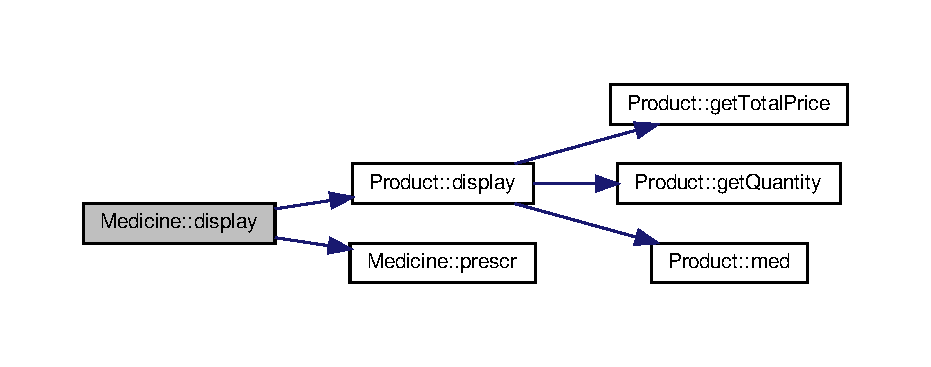
\includegraphics[width=350pt]{classMedicine_a42cabfcd2dd5f04b10e5a01d86f5ee60_cgraph}
\end{center}
\end{figure}
\mbox{\Hypertarget{classMedicine_aae7277cc1a23171b2d60225d0e11f24d}\label{classMedicine_aae7277cc1a23171b2d60225d0e11f24d}} 
\index{Medicine@{Medicine}!get\+Discount@{get\+Discount}}
\index{get\+Discount@{get\+Discount}!Medicine@{Medicine}}
\subsubsection{\texorpdfstring{get\+Discount()}{getDiscount()}}
{\footnotesize\ttfamily float Medicine\+::get\+Discount (\begin{DoxyParamCaption}{ }\end{DoxyParamCaption}) const}



Gets the Discount. 

\begin{DoxyReturn}{Returns}
The discount 
\end{DoxyReturn}
\mbox{\Hypertarget{classMedicine_a313a6ad362c0746ddb96425b097a8f77}\label{classMedicine_a313a6ad362c0746ddb96425b097a8f77}} 
\index{Medicine@{Medicine}!get\+Price\+With\+Discount@{get\+Price\+With\+Discount}}
\index{get\+Price\+With\+Discount@{get\+Price\+With\+Discount}!Medicine@{Medicine}}
\subsubsection{\texorpdfstring{get\+Price\+With\+Discount()}{getPriceWithDiscount()}}
{\footnotesize\ttfamily float Medicine\+::get\+Price\+With\+Discount (\begin{DoxyParamCaption}{ }\end{DoxyParamCaption}) const}



Calculates price with discount. 

\begin{DoxyReturn}{Returns}
Price with discount applied 
\end{DoxyReturn}
Here is the call graph for this function\+:\nopagebreak
\begin{figure}[H]
\begin{center}
\leavevmode
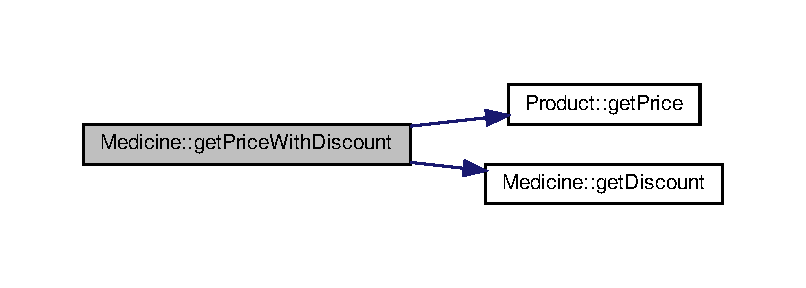
\includegraphics[width=350pt]{classMedicine_a313a6ad362c0746ddb96425b097a8f77_cgraph}
\end{center}
\end{figure}
\mbox{\Hypertarget{classMedicine_a502f519c44cfb89071af6a920fb773e3}\label{classMedicine_a502f519c44cfb89071af6a920fb773e3}} 
\index{Medicine@{Medicine}!prescr@{prescr}}
\index{prescr@{prescr}!Medicine@{Medicine}}
\subsubsection{\texorpdfstring{prescr()}{prescr()}}
{\footnotesize\ttfamily string Medicine\+::prescr (\begin{DoxyParamCaption}{ }\end{DoxyParamCaption}) const}

\mbox{\Hypertarget{classMedicine_ac69fcbbcfda660e3ee4df38282442dc4}\label{classMedicine_ac69fcbbcfda660e3ee4df38282442dc4}} 
\index{Medicine@{Medicine}!prescription\+Required@{prescription\+Required}}
\index{prescription\+Required@{prescription\+Required}!Medicine@{Medicine}}
\subsubsection{\texorpdfstring{prescription\+Required()}{prescriptionRequired()}}
{\footnotesize\ttfamily bool Medicine\+::prescription\+Required (\begin{DoxyParamCaption}{ }\end{DoxyParamCaption}) const}



\subsection{Friends And Related Function Documentation}
\mbox{\Hypertarget{classMedicine_ac59d59dad83c5b44d752d0dc6bdbf845}\label{classMedicine_ac59d59dad83c5b44d752d0dc6bdbf845}} 
\index{Medicine@{Medicine}!operator$<$$<$@{operator$<$$<$}}
\index{operator$<$$<$@{operator$<$$<$}!Medicine@{Medicine}}
\subsubsection{\texorpdfstring{operator$<$$<$}{operator<<}}
{\footnotesize\ttfamily ostream\& operator$<$$<$ (\begin{DoxyParamCaption}\item[{ostream \&}]{os,  }\item[{const \hyperlink{classMedicine}{Medicine} \&}]{m }\end{DoxyParamCaption})\hspace{0.3cm}{\ttfamily [friend]}}



Overload ostream operator $<$$<$ to write \hyperlink{classMedicine}{Medicine}\textquotesingle{}s info to an outstream. 


\begin{DoxyParams}{Parameters}
{\em os} & outstream\\
\hline
{\em m} & \hyperlink{classMedicine}{Medicine} to be written\\
\hline
\end{DoxyParams}
\begin{DoxyReturn}{Returns}
outstream 
\end{DoxyReturn}


\subsection{Member Data Documentation}
\mbox{\Hypertarget{classMedicine_a56e42f35d8edce81983df5837b6fee54}\label{classMedicine_a56e42f35d8edce81983df5837b6fee54}} 
\index{Medicine@{Medicine}!discount@{discount}}
\index{discount@{discount}!Medicine@{Medicine}}
\subsubsection{\texorpdfstring{discount}{discount}}
{\footnotesize\ttfamily float Medicine\+::discount\hspace{0.3cm}{\ttfamily [private]}}

\mbox{\Hypertarget{classMedicine_a10737b485d7f6e8b208ae5e26299333d}\label{classMedicine_a10737b485d7f6e8b208ae5e26299333d}} 
\index{Medicine@{Medicine}!prescription@{prescription}}
\index{prescription@{prescription}!Medicine@{Medicine}}
\subsubsection{\texorpdfstring{prescription}{prescription}}
{\footnotesize\ttfamily bool Medicine\+::prescription\hspace{0.3cm}{\ttfamily [private]}}



State discount on \hyperlink{classMedicine}{Medicine}. 

$<$ 

The documentation for this class was generated from the following files\+:\begin{DoxyCompactItemize}
\item 
src/\hyperlink{Medicine_8h}{Medicine.\+h}\item 
src/\hyperlink{Medicine_8cpp}{Medicine.\+cpp}\end{DoxyCompactItemize}

\hypertarget{classPerson}{}\section{Person Class Reference}
\label{classPerson}\index{Person@{Person}}


\hyperlink{classPerson}{Person} Class that represents a \hyperlink{classPerson}{Person} where is stored the person\textquotesingle{}s tax number.  




{\ttfamily \#include $<$Person.\+h$>$}



Inheritance diagram for Person\+:
\nopagebreak
\begin{figure}[H]
\begin{center}
\leavevmode
\includegraphics[width=214pt]{classPerson__inherit__graph}
\end{center}
\end{figure}


Collaboration diagram for Person\+:\nopagebreak
\begin{figure}[H]
\begin{center}
\leavevmode
\includegraphics[width=127pt]{classPerson__coll__graph}
\end{center}
\end{figure}
\subsection*{Public Member Functions}
\begin{DoxyCompactItemize}
\item 
\hyperlink{classPerson_aa4a247daff8ad28db9caac292dd2522b}{Person} (string n, string addr, unsigned int \hyperlink{classPerson_a55eea8ffb71b88d84ea43a6be15a2eb4}{contrib\+No})
\begin{DoxyCompactList}\small\item\em tax number of the \hyperlink{classPerson}{Person} \end{DoxyCompactList}\item 
unsigned int \hyperlink{classPerson_a8eb4c40211e1d1d3356d10df7f4ffcd7}{get\+Contrib\+No} () const
\begin{DoxyCompactList}\small\item\em Get the Contrib No object. \end{DoxyCompactList}\item 
bool \hyperlink{classPerson_a8b98ec6713875725a005f2b0ad19fa4c}{operator==} (const \hyperlink{classPerson}{Person} \&p)
\begin{DoxyCompactList}\small\item\em compares two person\textquotesingle{}s tax numbers \end{DoxyCompactList}\item 
bool \hyperlink{classPerson_aa61a8197d96d683b6c779a32382349cc}{operator$<$} (const \hyperlink{classPerson}{Person} \&p)
\begin{DoxyCompactList}\small\item\em compares two person\textquotesingle{}s name \end{DoxyCompactList}\end{DoxyCompactItemize}
\subsection*{Private Attributes}
\begin{DoxyCompactItemize}
\item 
unsigned int \hyperlink{classPerson_a55eea8ffb71b88d84ea43a6be15a2eb4}{contrib\+No}
\end{DoxyCompactItemize}
\subsection*{Friends}
\begin{DoxyCompactItemize}
\item 
ostream \& \hyperlink{classPerson_a520925d2df99c77933138568a48577dd}{operator$<$$<$} (ostream \&os, const \hyperlink{classPerson}{Person} \&p)
\begin{DoxyCompactList}\small\item\em writes \hyperlink{classPerson}{Person} p to outstream os \end{DoxyCompactList}\end{DoxyCompactItemize}


\subsection{Detailed Description}
\hyperlink{classPerson}{Person} Class that represents a \hyperlink{classPerson}{Person} where is stored the person\textquotesingle{}s tax number. 

Class for person. 

\subsection{Constructor \& Destructor Documentation}
\mbox{\Hypertarget{classPerson_aa4a247daff8ad28db9caac292dd2522b}\label{classPerson_aa4a247daff8ad28db9caac292dd2522b}} 
\index{Person@{Person}!Person@{Person}}
\index{Person@{Person}!Person@{Person}}
\subsubsection{\texorpdfstring{Person()}{Person()}}
{\footnotesize\ttfamily Person\+::\+Person (\begin{DoxyParamCaption}\item[{string}]{n,  }\item[{string}]{addr,  }\item[{unsigned int}]{contrib\+No }\end{DoxyParamCaption})}



tax number of the \hyperlink{classPerson}{Person} 

$<$ Construct a new \hyperlink{classPerson}{Person} object


\begin{DoxyParams}{Parameters}
{\em n} & The name of the \hyperlink{classPerson}{Person} to be created \\
\hline
{\em addr} & The adress of the \hyperlink{classPerson}{Person} be created \\
\hline
{\em contrib\+No} & The tax number of the \hyperlink{classPerson}{Person} to be created \\
\hline
\end{DoxyParams}


\subsection{Member Function Documentation}
\mbox{\Hypertarget{classPerson_a8eb4c40211e1d1d3356d10df7f4ffcd7}\label{classPerson_a8eb4c40211e1d1d3356d10df7f4ffcd7}} 
\index{Person@{Person}!get\+Contrib\+No@{get\+Contrib\+No}}
\index{get\+Contrib\+No@{get\+Contrib\+No}!Person@{Person}}
\subsubsection{\texorpdfstring{get\+Contrib\+No()}{getContribNo()}}
{\footnotesize\ttfamily unsigned int Person\+::get\+Contrib\+No (\begin{DoxyParamCaption}{ }\end{DoxyParamCaption}) const}



Get the Contrib No object. 

\begin{DoxyReturn}{Returns}
unsigned int person\textquotesingle{}s tax number 
\end{DoxyReturn}
\mbox{\Hypertarget{classPerson_aa61a8197d96d683b6c779a32382349cc}\label{classPerson_aa61a8197d96d683b6c779a32382349cc}} 
\index{Person@{Person}!operator$<$@{operator$<$}}
\index{operator$<$@{operator$<$}!Person@{Person}}
\subsubsection{\texorpdfstring{operator$<$()}{operator<()}}
{\footnotesize\ttfamily bool Person\+::operator$<$ (\begin{DoxyParamCaption}\item[{const \hyperlink{classPerson}{Person} \&}]{p }\end{DoxyParamCaption})}



compares two person\textquotesingle{}s name 


\begin{DoxyParams}{Parameters}
{\em p} & person to compare to\\
\hline
\end{DoxyParams}
\begin{DoxyReturn}{Returns}
true if \hyperlink{classPerson}{Person}\textquotesingle{}s name is alphabetical smaller than to p\textquotesingle{}s name 

false if \hyperlink{classPerson}{Person}\textquotesingle{}s name isn\textquotesingle{}t alphabetical smaller than to p\textquotesingle{}s name 
\end{DoxyReturn}
Here is the call graph for this function\+:\nopagebreak
\begin{figure}[H]
\begin{center}
\leavevmode
\includegraphics[width=299pt]{classPerson_aa61a8197d96d683b6c779a32382349cc_cgraph}
\end{center}
\end{figure}
\mbox{\Hypertarget{classPerson_a8b98ec6713875725a005f2b0ad19fa4c}\label{classPerson_a8b98ec6713875725a005f2b0ad19fa4c}} 
\index{Person@{Person}!operator==@{operator==}}
\index{operator==@{operator==}!Person@{Person}}
\subsubsection{\texorpdfstring{operator==()}{operator==()}}
{\footnotesize\ttfamily bool Person\+::operator== (\begin{DoxyParamCaption}\item[{const \hyperlink{classPerson}{Person} \&}]{p }\end{DoxyParamCaption})}



compares two person\textquotesingle{}s tax numbers 


\begin{DoxyParams}{Parameters}
{\em p} & person to compare to \\
\hline
\end{DoxyParams}
\begin{DoxyReturn}{Returns}
true if \hyperlink{classPerson}{Person}\textquotesingle{}s tax number is equal to p\textquotesingle{}s tax number 

false if \hyperlink{classPerson}{Person}\textquotesingle{}s tax number ism\textquotesingle{}t equal to p\textquotesingle{}s tax number 
\end{DoxyReturn}
Here is the call graph for this function\+:\nopagebreak
\begin{figure}[H]
\begin{center}
\leavevmode
\includegraphics[width=328pt]{classPerson_a8b98ec6713875725a005f2b0ad19fa4c_cgraph}
\end{center}
\end{figure}


\subsection{Friends And Related Function Documentation}
\mbox{\Hypertarget{classPerson_a520925d2df99c77933138568a48577dd}\label{classPerson_a520925d2df99c77933138568a48577dd}} 
\index{Person@{Person}!operator$<$$<$@{operator$<$$<$}}
\index{operator$<$$<$@{operator$<$$<$}!Person@{Person}}
\subsubsection{\texorpdfstring{operator$<$$<$}{operator<<}}
{\footnotesize\ttfamily ostream\& operator$<$$<$ (\begin{DoxyParamCaption}\item[{ostream \&}]{os,  }\item[{const \hyperlink{classPerson}{Person} \&}]{p }\end{DoxyParamCaption})\hspace{0.3cm}{\ttfamily [friend]}}



writes \hyperlink{classPerson}{Person} p to outstream os 


\begin{DoxyParams}{Parameters}
{\em os} & outstream\\
\hline
\end{DoxyParams}
param p \hyperlink{classPerson}{Person} Obj. to write

\begin{DoxyReturn}{Returns}
outstream 
\end{DoxyReturn}


\subsection{Member Data Documentation}
\mbox{\Hypertarget{classPerson_a55eea8ffb71b88d84ea43a6be15a2eb4}\label{classPerson_a55eea8ffb71b88d84ea43a6be15a2eb4}} 
\index{Person@{Person}!contrib\+No@{contrib\+No}}
\index{contrib\+No@{contrib\+No}!Person@{Person}}
\subsubsection{\texorpdfstring{contrib\+No}{contribNo}}
{\footnotesize\ttfamily unsigned int Person\+::contrib\+No\hspace{0.3cm}{\ttfamily [private]}}



The documentation for this class was generated from the following files\+:\begin{DoxyCompactItemize}
\item 
src/\hyperlink{Person_8h}{Person.\+h}\item 
src/\hyperlink{Person_8cpp}{Person.\+cpp}\end{DoxyCompactItemize}

\hypertarget{classPharmacy}{}\section{Pharmacy Class Reference}
\label{classPharmacy}\index{Pharmacy@{Pharmacy}}


\hyperlink{classPharmacy}{Pharmacy} Class that represents a \hyperlink{classPharmacy}{Pharmacy}.  




{\ttfamily \#include $<$Pharmacy.\+h$>$}



Inheritance diagram for Pharmacy\+:\nopagebreak
\begin{figure}[H]
\begin{center}
\leavevmode
\includegraphics[width=141pt]{classPharmacy__inherit__graph}
\end{center}
\end{figure}


Collaboration diagram for Pharmacy\+:\nopagebreak
\begin{figure}[H]
\begin{center}
\leavevmode
\includegraphics[width=141pt]{classPharmacy__coll__graph}
\end{center}
\end{figure}
\subsection*{Public Member Functions}
\begin{DoxyCompactItemize}
\item 
\hyperlink{classPharmacy_ad12ac7a309d2e77742508ecc7bee4453}{Pharmacy} (string n, string addr, string \hyperlink{classPharmacy_a620e101128be08b27f4401d53cfc39e6}{manager})
\begin{DoxyCompactList}\small\item\em Staff of the \hyperlink{classPharmacy}{Pharmacy} (all the members working in that \hyperlink{classPharmacy}{Pharmacy}) \end{DoxyCompactList}\item 
\hyperlink{classPharmacy_adb2b31d515bdf655ac3a952320a09680}{Pharmacy} (string n, string addr, string \hyperlink{classPharmacy_a620e101128be08b27f4401d53cfc39e6}{manager}, vector$<$ \hyperlink{classStaffMember}{Staff\+Member} $>$ sl)
\begin{DoxyCompactList}\small\item\em Construct a new \hyperlink{classPharmacy}{Pharmacy} object. \end{DoxyCompactList}\item 
vector$<$ \hyperlink{classStaffMember}{Staff\+Member} $>$ \hyperlink{classPharmacy_a030c21293a003be529663642a6825590}{get\+Staff} () const
\begin{DoxyCompactList}\small\item\em Get the Staff object. \end{DoxyCompactList}\item 
string \hyperlink{classPharmacy_acfa4217d82d6276e3e82991fdbb3fd13}{get\+Manager} () const
\begin{DoxyCompactList}\small\item\em Get the Manager object. \end{DoxyCompactList}\item 
string \hyperlink{classPharmacy_ac7e9631fe5f7e38e838a83a4118bbbf8}{get\+Info} () const
\begin{DoxyCompactList}\small\item\em Get the Info object. \end{DoxyCompactList}\item 
void \hyperlink{classPharmacy_a5c153e1ed72cfd0f824d43a1660c338d}{set\+Manager} (string \hyperlink{classEntity_afb45718695f537c330a463168616c262}{name})
\begin{DoxyCompactList}\small\item\em Sets the manager variable to a new one. \end{DoxyCompactList}\item 
void \hyperlink{classPharmacy_ac98f1404e96ea1560824afb612b1cab9}{add\+Staff} (\hyperlink{classStaffMember}{Staff\+Member} s)
\begin{DoxyCompactList}\small\item\em adds the Staff Member s the vector with all the Staff Members \end{DoxyCompactList}\item 
void \hyperlink{classPharmacy_ad1af6e62246f3060f922b4479d4d06bf}{remove\+Staff} (\hyperlink{classStaffMember}{Staff\+Member} s)
\begin{DoxyCompactList}\small\item\em removes the Staff Member s the vector with all the Staff Members \end{DoxyCompactList}\item 
bool \hyperlink{classPharmacy_acb5226880a626031aab93724949fa0e0}{operator==} (const \hyperlink{classPharmacy}{Pharmacy} \&p) const
\begin{DoxyCompactList}\small\item\em Compares two pharmacies and. \end{DoxyCompactList}\item 
void \hyperlink{classPharmacy_abdc810233f809eeab66fce0d443f1ba8}{set\+Staff\+Ph\+To\+None} ()
\begin{DoxyCompactList}\small\item\em Sets the pharmacy variable of the \hyperlink{classStaffMember}{Staff\+Member} \textquotesingle{}s from this pharmacy to None. Used when deleting a \hyperlink{classPharmacy}{Pharmacy}. \end{DoxyCompactList}\item 
bool \hyperlink{classPharmacy_a1fe770db0e60d644098750463cb2b8ee}{remove\+Staff} (string \hyperlink{classEntity_afb45718695f537c330a463168616c262}{name})
\begin{DoxyCompactList}\small\item\em Removes a certain \hyperlink{classStaffMember}{Staff\+Member} from this pharmacy. \end{DoxyCompactList}\item 
bool \hyperlink{classPharmacy_ababdb13d48f6e2c24e9a954f545bbeef}{contains\+Staff} (string \hyperlink{classEntity_afb45718695f537c330a463168616c262}{name})
\begin{DoxyCompactList}\small\item\em Checks if a \hyperlink{classStaffMember}{Staff\+Member} with a certain name exists in this \hyperlink{classPharmacy}{Pharmacy}. \end{DoxyCompactList}\item 
void \hyperlink{classPharmacy_addd2f907762d398ed28dba68eb4eaa66}{show\+Staffs\+Name} ()
\begin{DoxyCompactList}\small\item\em Displays the names of the \hyperlink{classStaffMember}{Staff\+Member} \textquotesingle{}s from this \hyperlink{classPharmacy}{Pharmacy}. \end{DoxyCompactList}\end{DoxyCompactItemize}
\subsection*{Private Attributes}
\begin{DoxyCompactItemize}
\item 
string \hyperlink{classPharmacy_a620e101128be08b27f4401d53cfc39e6}{manager}
\item 
vector$<$ \hyperlink{classStaffMember}{Staff\+Member} $>$ \hyperlink{classPharmacy_a5b515f5ef98dc2babdc48b8c937688a9}{staff}
\begin{DoxyCompactList}\small\item\em Manager of the \hyperlink{classPharmacy}{Pharmacy}. \end{DoxyCompactList}\end{DoxyCompactItemize}
\subsection*{Friends}
\begin{DoxyCompactItemize}
\item 
ostream \& \hyperlink{classPharmacy_aa75a7da96c11bdada029ebe3ecb397d6}{operator$<$$<$} (ostream \&os, const \hyperlink{classPharmacy}{Pharmacy} \&p)
\begin{DoxyCompactList}\small\item\em Overload outstream operator $<$$<$ to write a \hyperlink{classPharmacy}{Pharmacy} to an outstream. \end{DoxyCompactList}\end{DoxyCompactItemize}


\subsection{Detailed Description}
\hyperlink{classPharmacy}{Pharmacy} Class that represents a \hyperlink{classPharmacy}{Pharmacy}. 

\subsection{Constructor \& Destructor Documentation}
\mbox{\Hypertarget{classPharmacy_ad12ac7a309d2e77742508ecc7bee4453}\label{classPharmacy_ad12ac7a309d2e77742508ecc7bee4453}} 
\index{Pharmacy@{Pharmacy}!Pharmacy@{Pharmacy}}
\index{Pharmacy@{Pharmacy}!Pharmacy@{Pharmacy}}
\subsubsection{\texorpdfstring{Pharmacy()}{Pharmacy()}\hspace{0.1cm}{\footnotesize\ttfamily [1/2]}}
{\footnotesize\ttfamily Pharmacy\+::\+Pharmacy (\begin{DoxyParamCaption}\item[{string}]{n,  }\item[{string}]{addr,  }\item[{string}]{manager }\end{DoxyParamCaption})}



Staff of the \hyperlink{classPharmacy}{Pharmacy} (all the members working in that \hyperlink{classPharmacy}{Pharmacy}) 

$<$ Construct a new \hyperlink{classPharmacy}{Pharmacy} object


\begin{DoxyParams}{Parameters}
{\em n} & The name of the \hyperlink{classPharmacy}{Pharmacy} to be created \\
\hline
{\em addr} & The adress of the \hyperlink{classPharmacy}{Pharmacy} to be created \\
\hline
{\em manager} & The manager of the \hyperlink{classPharmacy}{Pharmacy} to be created \\
\hline
\end{DoxyParams}
\mbox{\Hypertarget{classPharmacy_adb2b31d515bdf655ac3a952320a09680}\label{classPharmacy_adb2b31d515bdf655ac3a952320a09680}} 
\index{Pharmacy@{Pharmacy}!Pharmacy@{Pharmacy}}
\index{Pharmacy@{Pharmacy}!Pharmacy@{Pharmacy}}
\subsubsection{\texorpdfstring{Pharmacy()}{Pharmacy()}\hspace{0.1cm}{\footnotesize\ttfamily [2/2]}}
{\footnotesize\ttfamily Pharmacy\+::\+Pharmacy (\begin{DoxyParamCaption}\item[{string}]{n,  }\item[{string}]{addr,  }\item[{string}]{manager,  }\item[{vector$<$ \hyperlink{classStaffMember}{Staff\+Member} $>$}]{sl }\end{DoxyParamCaption})}



Construct a new \hyperlink{classPharmacy}{Pharmacy} object. 


\begin{DoxyParams}{Parameters}
{\em n} & The name of the \hyperlink{classPharmacy}{Pharmacy} to be created \\
\hline
{\em addr} & The adress of the \hyperlink{classPharmacy}{Pharmacy} to be created \\
\hline
{\em sl} & All of the staff members of the \hyperlink{classPharmacy}{Pharmacy} to be created \\
\hline
\end{DoxyParams}


\subsection{Member Function Documentation}
\mbox{\Hypertarget{classPharmacy_ac98f1404e96ea1560824afb612b1cab9}\label{classPharmacy_ac98f1404e96ea1560824afb612b1cab9}} 
\index{Pharmacy@{Pharmacy}!add\+Staff@{add\+Staff}}
\index{add\+Staff@{add\+Staff}!Pharmacy@{Pharmacy}}
\subsubsection{\texorpdfstring{add\+Staff()}{addStaff()}}
{\footnotesize\ttfamily void Pharmacy\+::add\+Staff (\begin{DoxyParamCaption}\item[{\hyperlink{classStaffMember}{Staff\+Member}}]{s }\end{DoxyParamCaption})}



adds the Staff Member s the vector with all the Staff Members 


\begin{DoxyParams}{Parameters}
{\em s} & new Staff Member to be added \\
\hline
\end{DoxyParams}
\mbox{\Hypertarget{classPharmacy_ababdb13d48f6e2c24e9a954f545bbeef}\label{classPharmacy_ababdb13d48f6e2c24e9a954f545bbeef}} 
\index{Pharmacy@{Pharmacy}!contains\+Staff@{contains\+Staff}}
\index{contains\+Staff@{contains\+Staff}!Pharmacy@{Pharmacy}}
\subsubsection{\texorpdfstring{contains\+Staff()}{containsStaff()}}
{\footnotesize\ttfamily bool Pharmacy\+::contains\+Staff (\begin{DoxyParamCaption}\item[{string}]{name }\end{DoxyParamCaption})}



Checks if a \hyperlink{classStaffMember}{Staff\+Member} with a certain name exists in this \hyperlink{classPharmacy}{Pharmacy}. 


\begin{DoxyParams}{Parameters}
{\em name} & Name of the staff to be checked\\
\hline
\end{DoxyParams}
\begin{DoxyReturn}{Returns}
Boolean value of whether it contains the \hyperlink{classStaffMember}{Staff\+Member} or not 
\end{DoxyReturn}
Here is the call graph for this function\+:\nopagebreak
\begin{figure}[H]
\begin{center}
\leavevmode
\includegraphics[width=329pt]{classPharmacy_ababdb13d48f6e2c24e9a954f545bbeef_cgraph}
\end{center}
\end{figure}
\mbox{\Hypertarget{classPharmacy_ac7e9631fe5f7e38e838a83a4118bbbf8}\label{classPharmacy_ac7e9631fe5f7e38e838a83a4118bbbf8}} 
\index{Pharmacy@{Pharmacy}!get\+Info@{get\+Info}}
\index{get\+Info@{get\+Info}!Pharmacy@{Pharmacy}}
\subsubsection{\texorpdfstring{get\+Info()}{getInfo()}}
{\footnotesize\ttfamily string Pharmacy\+::get\+Info (\begin{DoxyParamCaption}{ }\end{DoxyParamCaption}) const}



Get the Info object. 

\begin{DoxyReturn}{Returns}
string prints all the the \hyperlink{classPharmacy}{Pharmacy}\textquotesingle{}s information 
\end{DoxyReturn}
\mbox{\Hypertarget{classPharmacy_acfa4217d82d6276e3e82991fdbb3fd13}\label{classPharmacy_acfa4217d82d6276e3e82991fdbb3fd13}} 
\index{Pharmacy@{Pharmacy}!get\+Manager@{get\+Manager}}
\index{get\+Manager@{get\+Manager}!Pharmacy@{Pharmacy}}
\subsubsection{\texorpdfstring{get\+Manager()}{getManager()}}
{\footnotesize\ttfamily string Pharmacy\+::get\+Manager (\begin{DoxyParamCaption}{ }\end{DoxyParamCaption}) const}



Get the Manager object. 

\begin{DoxyReturn}{Returns}
string the manager of the \hyperlink{classPharmacy}{Pharmacy} 
\end{DoxyReturn}
\mbox{\Hypertarget{classPharmacy_a030c21293a003be529663642a6825590}\label{classPharmacy_a030c21293a003be529663642a6825590}} 
\index{Pharmacy@{Pharmacy}!get\+Staff@{get\+Staff}}
\index{get\+Staff@{get\+Staff}!Pharmacy@{Pharmacy}}
\subsubsection{\texorpdfstring{get\+Staff()}{getStaff()}}
{\footnotesize\ttfamily vector$<$ \hyperlink{classStaffMember}{Staff\+Member} $>$ Pharmacy\+::get\+Staff (\begin{DoxyParamCaption}{ }\end{DoxyParamCaption}) const}



Get the Staff object. 

\begin{DoxyReturn}{Returns}
vector$<$\+Staff\+Member$>$ the staff members of the \hyperlink{classPharmacy}{Pharmacy} 
\end{DoxyReturn}
\mbox{\Hypertarget{classPharmacy_acb5226880a626031aab93724949fa0e0}\label{classPharmacy_acb5226880a626031aab93724949fa0e0}} 
\index{Pharmacy@{Pharmacy}!operator==@{operator==}}
\index{operator==@{operator==}!Pharmacy@{Pharmacy}}
\subsubsection{\texorpdfstring{operator==()}{operator==()}}
{\footnotesize\ttfamily bool Pharmacy\+::operator== (\begin{DoxyParamCaption}\item[{const \hyperlink{classPharmacy}{Pharmacy} \&}]{p }\end{DoxyParamCaption}) const}



Compares two pharmacies and. 


\begin{DoxyParams}{Parameters}
{\em p} & \hyperlink{classPharmacy}{Pharmacy} to be compared with\\
\hline
\end{DoxyParams}
\begin{DoxyReturn}{Returns}
Boolean value of whether they\textquotesingle{}re equal or not 
\end{DoxyReturn}
Here is the call graph for this function\+:\nopagebreak
\begin{figure}[H]
\begin{center}
\leavevmode
\includegraphics[width=318pt]{classPharmacy_acb5226880a626031aab93724949fa0e0_cgraph}
\end{center}
\end{figure}
\mbox{\Hypertarget{classPharmacy_ad1af6e62246f3060f922b4479d4d06bf}\label{classPharmacy_ad1af6e62246f3060f922b4479d4d06bf}} 
\index{Pharmacy@{Pharmacy}!remove\+Staff@{remove\+Staff}}
\index{remove\+Staff@{remove\+Staff}!Pharmacy@{Pharmacy}}
\subsubsection{\texorpdfstring{remove\+Staff()}{removeStaff()}\hspace{0.1cm}{\footnotesize\ttfamily [1/2]}}
{\footnotesize\ttfamily void Pharmacy\+::remove\+Staff (\begin{DoxyParamCaption}\item[{\hyperlink{classStaffMember}{Staff\+Member}}]{s }\end{DoxyParamCaption})}



removes the Staff Member s the vector with all the Staff Members 


\begin{DoxyParams}{Parameters}
{\em s} & Staff Member to be removed \\
\hline
\end{DoxyParams}
\mbox{\Hypertarget{classPharmacy_a1fe770db0e60d644098750463cb2b8ee}\label{classPharmacy_a1fe770db0e60d644098750463cb2b8ee}} 
\index{Pharmacy@{Pharmacy}!remove\+Staff@{remove\+Staff}}
\index{remove\+Staff@{remove\+Staff}!Pharmacy@{Pharmacy}}
\subsubsection{\texorpdfstring{remove\+Staff()}{removeStaff()}\hspace{0.1cm}{\footnotesize\ttfamily [2/2]}}
{\footnotesize\ttfamily bool Pharmacy\+::remove\+Staff (\begin{DoxyParamCaption}\item[{string}]{name }\end{DoxyParamCaption})}



Removes a certain \hyperlink{classStaffMember}{Staff\+Member} from this pharmacy. 


\begin{DoxyParams}{Parameters}
{\em name} & Name of the staff to be removed\\
\hline
\end{DoxyParams}
\begin{DoxyReturn}{Returns}
Boolean value of whether it was removed or not 
\end{DoxyReturn}
\mbox{\Hypertarget{classPharmacy_a5c153e1ed72cfd0f824d43a1660c338d}\label{classPharmacy_a5c153e1ed72cfd0f824d43a1660c338d}} 
\index{Pharmacy@{Pharmacy}!set\+Manager@{set\+Manager}}
\index{set\+Manager@{set\+Manager}!Pharmacy@{Pharmacy}}
\subsubsection{\texorpdfstring{set\+Manager()}{setManager()}}
{\footnotesize\ttfamily void Pharmacy\+::set\+Manager (\begin{DoxyParamCaption}\item[{string}]{name }\end{DoxyParamCaption})}



Sets the manager variable to a new one. 


\begin{DoxyParams}{Parameters}
{\em name} & Name of the new manager \\
\hline
\end{DoxyParams}
Here is the call graph for this function\+:\nopagebreak
\begin{figure}[H]
\begin{center}
\leavevmode
\includegraphics[width=322pt]{classPharmacy_a5c153e1ed72cfd0f824d43a1660c338d_cgraph}
\end{center}
\end{figure}
\mbox{\Hypertarget{classPharmacy_abdc810233f809eeab66fce0d443f1ba8}\label{classPharmacy_abdc810233f809eeab66fce0d443f1ba8}} 
\index{Pharmacy@{Pharmacy}!set\+Staff\+Ph\+To\+None@{set\+Staff\+Ph\+To\+None}}
\index{set\+Staff\+Ph\+To\+None@{set\+Staff\+Ph\+To\+None}!Pharmacy@{Pharmacy}}
\subsubsection{\texorpdfstring{set\+Staff\+Ph\+To\+None()}{setStaffPhToNone()}}
{\footnotesize\ttfamily void Pharmacy\+::set\+Staff\+Ph\+To\+None (\begin{DoxyParamCaption}{ }\end{DoxyParamCaption})}



Sets the pharmacy variable of the \hyperlink{classStaffMember}{Staff\+Member} \textquotesingle{}s from this pharmacy to None. Used when deleting a \hyperlink{classPharmacy}{Pharmacy}. 

\mbox{\Hypertarget{classPharmacy_addd2f907762d398ed28dba68eb4eaa66}\label{classPharmacy_addd2f907762d398ed28dba68eb4eaa66}} 
\index{Pharmacy@{Pharmacy}!show\+Staffs\+Name@{show\+Staffs\+Name}}
\index{show\+Staffs\+Name@{show\+Staffs\+Name}!Pharmacy@{Pharmacy}}
\subsubsection{\texorpdfstring{show\+Staffs\+Name()}{showStaffsName()}}
{\footnotesize\ttfamily void Pharmacy\+::show\+Staffs\+Name (\begin{DoxyParamCaption}{ }\end{DoxyParamCaption})}



Displays the names of the \hyperlink{classStaffMember}{Staff\+Member} \textquotesingle{}s from this \hyperlink{classPharmacy}{Pharmacy}. 



\subsection{Friends And Related Function Documentation}
\mbox{\Hypertarget{classPharmacy_aa75a7da96c11bdada029ebe3ecb397d6}\label{classPharmacy_aa75a7da96c11bdada029ebe3ecb397d6}} 
\index{Pharmacy@{Pharmacy}!operator$<$$<$@{operator$<$$<$}}
\index{operator$<$$<$@{operator$<$$<$}!Pharmacy@{Pharmacy}}
\subsubsection{\texorpdfstring{operator$<$$<$}{operator<<}}
{\footnotesize\ttfamily ostream\& operator$<$$<$ (\begin{DoxyParamCaption}\item[{ostream \&}]{os,  }\item[{const \hyperlink{classPharmacy}{Pharmacy} \&}]{p }\end{DoxyParamCaption})\hspace{0.3cm}{\ttfamily [friend]}}



Overload outstream operator $<$$<$ to write a \hyperlink{classPharmacy}{Pharmacy} to an outstream. 


\begin{DoxyParams}{Parameters}
{\em os} & Outstream\\
\hline
{\em p} & \hyperlink{classPharmacy}{Pharmacy} to be written\\
\hline
\end{DoxyParams}
\begin{DoxyReturn}{Returns}
Outstream 
\end{DoxyReturn}


\subsection{Member Data Documentation}
\mbox{\Hypertarget{classPharmacy_a620e101128be08b27f4401d53cfc39e6}\label{classPharmacy_a620e101128be08b27f4401d53cfc39e6}} 
\index{Pharmacy@{Pharmacy}!manager@{manager}}
\index{manager@{manager}!Pharmacy@{Pharmacy}}
\subsubsection{\texorpdfstring{manager}{manager}}
{\footnotesize\ttfamily string Pharmacy\+::manager\hspace{0.3cm}{\ttfamily [private]}}

\mbox{\Hypertarget{classPharmacy_a5b515f5ef98dc2babdc48b8c937688a9}\label{classPharmacy_a5b515f5ef98dc2babdc48b8c937688a9}} 
\index{Pharmacy@{Pharmacy}!staff@{staff}}
\index{staff@{staff}!Pharmacy@{Pharmacy}}
\subsubsection{\texorpdfstring{staff}{staff}}
{\footnotesize\ttfamily vector$<$\hyperlink{classStaffMember}{Staff\+Member}$>$ Pharmacy\+::staff\hspace{0.3cm}{\ttfamily [private]}}



Manager of the \hyperlink{classPharmacy}{Pharmacy}. 

$<$ 

The documentation for this class was generated from the following files\+:\begin{DoxyCompactItemize}
\item 
src/\hyperlink{Pharmacy_8h}{Pharmacy.\+h}\item 
src/\hyperlink{Pharmacy_8cpp}{Pharmacy.\+cpp}\end{DoxyCompactItemize}

\hypertarget{classPrescription}{}\section{Prescription Class Reference}
\label{classPrescription}\index{Prescription@{Prescription}}


\hyperlink{classPrescription}{Prescription} Class that represents a prescription where are stored the number, client, doctor and products os the prescription.  




{\ttfamily \#include $<$Prescription.\+h$>$}

\subsection*{Public Member Functions}
\begin{DoxyCompactItemize}
\item 
\hyperlink{classPrescription_a8dce6fbdb5b57a18c45de8992bf5d600}{Prescription} ()
\begin{DoxyCompactList}\small\item\em Construct a new \hyperlink{classPrescription}{Prescription} object. \end{DoxyCompactList}\item 
\hyperlink{classPrescription_a7be35e4e8ddb08878fd4fcbf308f9d2b}{Prescription} (int \hyperlink{classPrescription_a4b3dcfe55dff479143e63cf7778ffa12}{number}, string \hyperlink{classPrescription_a3a2d122c0229cd7985595cae3ab497c3}{client}, string \hyperlink{classPrescription_abf1e3c58a207e521294815884ffc6682}{doctor}, string \hyperlink{classPrescription_ab9556fbe876105624867e2f360617688}{product})
\begin{DoxyCompactList}\small\item\em Construct a new \hyperlink{classPrescription}{Prescription} object. \end{DoxyCompactList}\item 
virtual \hyperlink{classPrescription_a79779a7a4954ae3566411772a5313a88}{$\sim$\+Prescription} ()
\begin{DoxyCompactList}\small\item\em Destroy the \hyperlink{classPrescription}{Prescription} object. \end{DoxyCompactList}\item 
int \hyperlink{classPrescription_a6a89f632894bee1e959973d26f0b4cc8}{get\+Number} () const
\begin{DoxyCompactList}\small\item\em Get the Number object. \end{DoxyCompactList}\item 
const string \& \hyperlink{classPrescription_aaf2631c310511731d1538b9129b1ad04}{get\+Client} () const
\begin{DoxyCompactList}\small\item\em Get the \hyperlink{classClient}{Client} object. \end{DoxyCompactList}\item 
const string \& \hyperlink{classPrescription_aba0ddace1c50e0f708d1f8e427263e0f}{get\+Doctor} () const
\begin{DoxyCompactList}\small\item\em Get the Doctor object. \end{DoxyCompactList}\item 
string \hyperlink{classPrescription_aca98893524a101d4b42fd5ef4ea1ed51}{get\+Product} () const
\item 
void \hyperlink{classPrescription_a2c0f9433fda32c1ef8d4e96ff3b965b0}{set\+Client} (string c)
\begin{DoxyCompactList}\small\item\em Sets the client. \end{DoxyCompactList}\item 
void \hyperlink{classPrescription_ac2623f2ff21c5b0b454913c66e5f40a0}{set\+Dr} (string c)
\begin{DoxyCompactList}\small\item\em Sets the Doctor. \end{DoxyCompactList}\item 
void \hyperlink{classPrescription_a2594567d8bbb03cf18710db571c0cb64}{set\+Product} (string c)
\begin{DoxyCompactList}\small\item\em Sets the \hyperlink{classProduct}{Product}. \end{DoxyCompactList}\end{DoxyCompactItemize}
\subsection*{Private Attributes}
\begin{DoxyCompactItemize}
\item 
int \hyperlink{classPrescription_a4b3dcfe55dff479143e63cf7778ffa12}{number}
\item 
string \hyperlink{classPrescription_a3a2d122c0229cd7985595cae3ab497c3}{client}
\item 
string \hyperlink{classPrescription_abf1e3c58a207e521294815884ffc6682}{doctor}
\item 
string \hyperlink{classPrescription_ab9556fbe876105624867e2f360617688}{product}
\end{DoxyCompactItemize}
\subsection*{Friends}
\begin{DoxyCompactItemize}
\item 
ostream \& \hyperlink{classPrescription_a3daeb997a2f3f9666159cf018d0d1c28}{operator$<$$<$} (ostream \&os, const \hyperlink{classPrescription}{Prescription} \&p)
\item 
ostream \& \hyperlink{classPrescription_a3daeb997a2f3f9666159cf018d0d1c28}{operator$<$$<$} (ostream \&os, const \hyperlink{classPrescription}{Prescription} \&p)
\begin{DoxyCompactList}\small\item\em Overload ostream $<$$<$ operator to write Prescripiton to an outstream. \end{DoxyCompactList}\end{DoxyCompactItemize}


\subsection{Detailed Description}
\hyperlink{classPrescription}{Prescription} Class that represents a prescription where are stored the number, client, doctor and products os the prescription. 

\subsection{Constructor \& Destructor Documentation}
\mbox{\Hypertarget{classPrescription_a8dce6fbdb5b57a18c45de8992bf5d600}\label{classPrescription_a8dce6fbdb5b57a18c45de8992bf5d600}} 
\index{Prescription@{Prescription}!Prescription@{Prescription}}
\index{Prescription@{Prescription}!Prescription@{Prescription}}
\subsubsection{\texorpdfstring{Prescription()}{Prescription()}\hspace{0.1cm}{\footnotesize\ttfamily [1/2]}}
{\footnotesize\ttfamily Prescription\+::\+Prescription (\begin{DoxyParamCaption}{ }\end{DoxyParamCaption})}



Construct a new \hyperlink{classPrescription}{Prescription} object. 

\mbox{\Hypertarget{classPrescription_a7be35e4e8ddb08878fd4fcbf308f9d2b}\label{classPrescription_a7be35e4e8ddb08878fd4fcbf308f9d2b}} 
\index{Prescription@{Prescription}!Prescription@{Prescription}}
\index{Prescription@{Prescription}!Prescription@{Prescription}}
\subsubsection{\texorpdfstring{Prescription()}{Prescription()}\hspace{0.1cm}{\footnotesize\ttfamily [2/2]}}
{\footnotesize\ttfamily Prescription\+::\+Prescription (\begin{DoxyParamCaption}\item[{int}]{number,  }\item[{string}]{client,  }\item[{string}]{doctor,  }\item[{string}]{product }\end{DoxyParamCaption})}



Construct a new \hyperlink{classPrescription}{Prescription} object. 


\begin{DoxyParams}{Parameters}
{\em number} & number of the \hyperlink{classPrescription}{Prescription} to be created \\
\hline
{\em client} & \hyperlink{classClient}{Client} that owns the prescription to be created \\
\hline
{\em doctor} & Doctor that wrote the prescription to be created \\
\hline
\end{DoxyParams}
\mbox{\Hypertarget{classPrescription_a79779a7a4954ae3566411772a5313a88}\label{classPrescription_a79779a7a4954ae3566411772a5313a88}} 
\index{Prescription@{Prescription}!````~Prescription@{$\sim$\+Prescription}}
\index{````~Prescription@{$\sim$\+Prescription}!Prescription@{Prescription}}
\subsubsection{\texorpdfstring{$\sim$\+Prescription()}{~Prescription()}}
{\footnotesize\ttfamily Prescription\+::$\sim$\+Prescription (\begin{DoxyParamCaption}{ }\end{DoxyParamCaption})\hspace{0.3cm}{\ttfamily [virtual]}}



Destroy the \hyperlink{classPrescription}{Prescription} object. 



\subsection{Member Function Documentation}
\mbox{\Hypertarget{classPrescription_aaf2631c310511731d1538b9129b1ad04}\label{classPrescription_aaf2631c310511731d1538b9129b1ad04}} 
\index{Prescription@{Prescription}!get\+Client@{get\+Client}}
\index{get\+Client@{get\+Client}!Prescription@{Prescription}}
\subsubsection{\texorpdfstring{get\+Client()}{getClient()}}
{\footnotesize\ttfamily const string \& Prescription\+::get\+Client (\begin{DoxyParamCaption}{ }\end{DoxyParamCaption}) const}



Get the \hyperlink{classClient}{Client} object. 

\begin{DoxyReturn}{Returns}
const string\& \hyperlink{classPrescription}{Prescription}\textquotesingle{}s \hyperlink{classClient}{Client} 
\end{DoxyReturn}
\mbox{\Hypertarget{classPrescription_aba0ddace1c50e0f708d1f8e427263e0f}\label{classPrescription_aba0ddace1c50e0f708d1f8e427263e0f}} 
\index{Prescription@{Prescription}!get\+Doctor@{get\+Doctor}}
\index{get\+Doctor@{get\+Doctor}!Prescription@{Prescription}}
\subsubsection{\texorpdfstring{get\+Doctor()}{getDoctor()}}
{\footnotesize\ttfamily const string\& Prescription\+::get\+Doctor (\begin{DoxyParamCaption}{ }\end{DoxyParamCaption}) const}



Get the Doctor object. 

\begin{DoxyReturn}{Returns}
const string\& \hyperlink{classPrescription}{Prescription}\textquotesingle{}s Doctor 
\end{DoxyReturn}
\mbox{\Hypertarget{classPrescription_a6a89f632894bee1e959973d26f0b4cc8}\label{classPrescription_a6a89f632894bee1e959973d26f0b4cc8}} 
\index{Prescription@{Prescription}!get\+Number@{get\+Number}}
\index{get\+Number@{get\+Number}!Prescription@{Prescription}}
\subsubsection{\texorpdfstring{get\+Number()}{getNumber()}}
{\footnotesize\ttfamily int Prescription\+::get\+Number (\begin{DoxyParamCaption}{ }\end{DoxyParamCaption}) const}



Get the Number object. 

\begin{DoxyReturn}{Returns}
int \hyperlink{classPrescription}{Prescription}\textquotesingle{}s number 
\end{DoxyReturn}
\mbox{\Hypertarget{classPrescription_aca98893524a101d4b42fd5ef4ea1ed51}\label{classPrescription_aca98893524a101d4b42fd5ef4ea1ed51}} 
\index{Prescription@{Prescription}!get\+Product@{get\+Product}}
\index{get\+Product@{get\+Product}!Prescription@{Prescription}}
\subsubsection{\texorpdfstring{get\+Product()}{getProduct()}}
{\footnotesize\ttfamily string Prescription\+::get\+Product (\begin{DoxyParamCaption}{ }\end{DoxyParamCaption}) const}

\mbox{\Hypertarget{classPrescription_a2c0f9433fda32c1ef8d4e96ff3b965b0}\label{classPrescription_a2c0f9433fda32c1ef8d4e96ff3b965b0}} 
\index{Prescription@{Prescription}!set\+Client@{set\+Client}}
\index{set\+Client@{set\+Client}!Prescription@{Prescription}}
\subsubsection{\texorpdfstring{set\+Client()}{setClient()}}
{\footnotesize\ttfamily void Prescription\+::set\+Client (\begin{DoxyParamCaption}\item[{string}]{c }\end{DoxyParamCaption})}



Sets the client. 


\begin{DoxyParams}{Parameters}
{\em c} & \hyperlink{classClient}{Client} Name \\
\hline
\end{DoxyParams}
\mbox{\Hypertarget{classPrescription_ac2623f2ff21c5b0b454913c66e5f40a0}\label{classPrescription_ac2623f2ff21c5b0b454913c66e5f40a0}} 
\index{Prescription@{Prescription}!set\+Dr@{set\+Dr}}
\index{set\+Dr@{set\+Dr}!Prescription@{Prescription}}
\subsubsection{\texorpdfstring{set\+Dr()}{setDr()}}
{\footnotesize\ttfamily void Prescription\+::set\+Dr (\begin{DoxyParamCaption}\item[{string}]{c }\end{DoxyParamCaption})}



Sets the Doctor. 


\begin{DoxyParams}{Parameters}
{\em c} & Doctor Name \\
\hline
\end{DoxyParams}
\mbox{\Hypertarget{classPrescription_a2594567d8bbb03cf18710db571c0cb64}\label{classPrescription_a2594567d8bbb03cf18710db571c0cb64}} 
\index{Prescription@{Prescription}!set\+Product@{set\+Product}}
\index{set\+Product@{set\+Product}!Prescription@{Prescription}}
\subsubsection{\texorpdfstring{set\+Product()}{setProduct()}}
{\footnotesize\ttfamily void Prescription\+::set\+Product (\begin{DoxyParamCaption}\item[{string}]{c }\end{DoxyParamCaption})}



Sets the \hyperlink{classProduct}{Product}. 


\begin{DoxyParams}{Parameters}
{\em c} & \hyperlink{classProduct}{Product} Name \\
\hline
\end{DoxyParams}


\subsection{Friends And Related Function Documentation}
\mbox{\Hypertarget{classPrescription_a3daeb997a2f3f9666159cf018d0d1c28}\label{classPrescription_a3daeb997a2f3f9666159cf018d0d1c28}} 
\index{Prescription@{Prescription}!operator$<$$<$@{operator$<$$<$}}
\index{operator$<$$<$@{operator$<$$<$}!Prescription@{Prescription}}
\subsubsection{\texorpdfstring{operator$<$$<$}{operator<<}\hspace{0.1cm}{\footnotesize\ttfamily [1/2]}}
{\footnotesize\ttfamily ostream\& operator$<$$<$ (\begin{DoxyParamCaption}\item[{ostream \&}]{os,  }\item[{const \hyperlink{classPrescription}{Prescription} \&}]{p }\end{DoxyParamCaption})\hspace{0.3cm}{\ttfamily [friend]}}

\mbox{\Hypertarget{classPrescription_a3daeb997a2f3f9666159cf018d0d1c28}\label{classPrescription_a3daeb997a2f3f9666159cf018d0d1c28}} 
\index{Prescription@{Prescription}!operator$<$$<$@{operator$<$$<$}}
\index{operator$<$$<$@{operator$<$$<$}!Prescription@{Prescription}}
\subsubsection{\texorpdfstring{operator$<$$<$}{operator<<}\hspace{0.1cm}{\footnotesize\ttfamily [2/2]}}
{\footnotesize\ttfamily ostream\& operator$<$$<$ (\begin{DoxyParamCaption}\item[{ostream \&}]{os,  }\item[{const \hyperlink{classPrescription}{Prescription} \&}]{p }\end{DoxyParamCaption})\hspace{0.3cm}{\ttfamily [friend]}}



Overload ostream $<$$<$ operator to write Prescripiton to an outstream. 


\begin{DoxyParams}{Parameters}
{\em os} & Outstream\\
\hline
{\em p} & \hyperlink{classPrescription}{Prescription} to be written\\
\hline
\end{DoxyParams}
\begin{DoxyReturn}{Returns}
Outstream 
\end{DoxyReturn}


\subsection{Member Data Documentation}
\mbox{\Hypertarget{classPrescription_a3a2d122c0229cd7985595cae3ab497c3}\label{classPrescription_a3a2d122c0229cd7985595cae3ab497c3}} 
\index{Prescription@{Prescription}!client@{client}}
\index{client@{client}!Prescription@{Prescription}}
\subsubsection{\texorpdfstring{client}{client}}
{\footnotesize\ttfamily string Prescription\+::client\hspace{0.3cm}{\ttfamily [private]}}

\mbox{\Hypertarget{classPrescription_abf1e3c58a207e521294815884ffc6682}\label{classPrescription_abf1e3c58a207e521294815884ffc6682}} 
\index{Prescription@{Prescription}!doctor@{doctor}}
\index{doctor@{doctor}!Prescription@{Prescription}}
\subsubsection{\texorpdfstring{doctor}{doctor}}
{\footnotesize\ttfamily string Prescription\+::doctor\hspace{0.3cm}{\ttfamily [private]}}

\mbox{\Hypertarget{classPrescription_a4b3dcfe55dff479143e63cf7778ffa12}\label{classPrescription_a4b3dcfe55dff479143e63cf7778ffa12}} 
\index{Prescription@{Prescription}!number@{number}}
\index{number@{number}!Prescription@{Prescription}}
\subsubsection{\texorpdfstring{number}{number}}
{\footnotesize\ttfamily int Prescription\+::number\hspace{0.3cm}{\ttfamily [private]}}

\mbox{\Hypertarget{classPrescription_ab9556fbe876105624867e2f360617688}\label{classPrescription_ab9556fbe876105624867e2f360617688}} 
\index{Prescription@{Prescription}!product@{product}}
\index{product@{product}!Prescription@{Prescription}}
\subsubsection{\texorpdfstring{product}{product}}
{\footnotesize\ttfamily string Prescription\+::product\hspace{0.3cm}{\ttfamily [private]}}



The documentation for this class was generated from the following files\+:\begin{DoxyCompactItemize}
\item 
src/\hyperlink{Prescription_8h}{Prescription.\+h}\item 
src/\hyperlink{Prescription_8cpp}{Prescription.\+cpp}\end{DoxyCompactItemize}

\hypertarget{classProduct}{}\section{Product Class Reference}
\label{classProduct}\index{Product@{Product}}


\hyperlink{classProduct}{Product} Class that represents a prescription where are stored the number, client, doctor and products os the prescription.  




{\ttfamily \#include $<$Product.\+h$>$}



Inheritance diagram for Product\+:\nopagebreak
\begin{figure}[H]
\begin{center}
\leavevmode
\includegraphics[width=136pt]{classProduct__inherit__graph}
\end{center}
\end{figure}
\subsection*{Public Member Functions}
\begin{DoxyCompactItemize}
\item 
\hyperlink{classProduct_a847c1d85e67ce387166a597579a55135}{Product} ()
\begin{DoxyCompactList}\small\item\em Construct a new \hyperlink{classProduct}{Product} object. \end{DoxyCompactList}\item 
\hyperlink{classProduct_af5787b56a6be5a1807ceb7999c6adb6a}{Product} (string \hyperlink{classProduct_acc9bddcf74112d85a6dc231db2269b8d}{name}, string \hyperlink{classProduct_ac39d552b24ce60549271a85aea3f5ed0}{description}, float \hyperlink{classProduct_ad1fd6ee6c8653bf81898668b1d01b05d}{price}, int \hyperlink{classProduct_a299430b8756aba9f6d44af46831791cc}{quantity}, float \hyperlink{classProduct_ac772b7a57928ccfdb02309bde2e4fa33}{iva}, int \hyperlink{classProduct_acf4c1bb9d62717e3b2ecaaf7ec5dffd7}{code}, bool m)
\begin{DoxyCompactList}\small\item\em Construct a new \hyperlink{classProduct}{Product} object. \end{DoxyCompactList}\item 
int \hyperlink{classProduct_ada9a32ed7891875b3ccd8e064aad6492}{get\+Code} () const
\begin{DoxyCompactList}\small\item\em Destroy the \hyperlink{classProduct}{Product} object. \end{DoxyCompactList}\item 
const string \& \hyperlink{classProduct_afffde8c14c3bca709543cea274d67e7c}{get\+Description} () const
\begin{DoxyCompactList}\small\item\em Get the Description object. \end{DoxyCompactList}\item 
float \hyperlink{classProduct_a50605c5d457a7400a8dd5a0848480297}{get\+Iva} () const
\begin{DoxyCompactList}\small\item\em Get the Iva object. \end{DoxyCompactList}\item 
const string \& \hyperlink{classProduct_acbf3d46720bb1a0d16e49663b73b803d}{get\+Name} () const
\begin{DoxyCompactList}\small\item\em Get the Name object. \end{DoxyCompactList}\item 
float \hyperlink{classProduct_a0aaea95b8d3241b3758246254b8575e2}{get\+Price} () const
\begin{DoxyCompactList}\small\item\em Get the Price object. \end{DoxyCompactList}\item 
float \hyperlink{classProduct_a732aca2574f7a39e3a90837e0240e81f}{get\+Total\+Price} () const
\begin{DoxyCompactList}\small\item\em Get the Total Price object. \end{DoxyCompactList}\item 
virtual string \hyperlink{classProduct_a2f411b12652a6b7b6194fcdbab3a1fb3}{display} () const
\begin{DoxyCompactList}\small\item\em Write product info to string. \end{DoxyCompactList}\item 
bool \hyperlink{classProduct_a3a703454d7777191ad9282b38bce15e1}{get\+Medicine} () const
\item 
int \hyperlink{classProduct_a6a449b90b669aa4380d229b44eca686f}{get\+Quantity} () const
\item 
string \hyperlink{classProduct_aa2ccc7b6aa44a0bf10694b18f910dfa1}{med} () const
\item 
bool \hyperlink{classProduct_add7a6d09de7f21ca5d8a0228461ad6ae}{operator$<$} (const \hyperlink{classProduct}{Product} \&prod1) const
\end{DoxyCompactItemize}
\subsection*{Private Attributes}
\begin{DoxyCompactItemize}
\item 
string \hyperlink{classProduct_acc9bddcf74112d85a6dc231db2269b8d}{name}
\item 
string \hyperlink{classProduct_ac39d552b24ce60549271a85aea3f5ed0}{description}
\begin{DoxyCompactList}\small\item\em Name of the \hyperlink{classProduct}{Product}. \end{DoxyCompactList}\item 
float \hyperlink{classProduct_ad1fd6ee6c8653bf81898668b1d01b05d}{price}
\begin{DoxyCompactList}\small\item\em Description of the \hyperlink{classProduct}{Product}. \end{DoxyCompactList}\item 
float \hyperlink{classProduct_ac772b7a57928ccfdb02309bde2e4fa33}{iva}
\begin{DoxyCompactList}\small\item\em Price of the \hyperlink{classProduct}{Product}. \end{DoxyCompactList}\item 
int \hyperlink{classProduct_acf4c1bb9d62717e3b2ecaaf7ec5dffd7}{code}
\begin{DoxyCompactList}\small\item\em Iva of the \hyperlink{classProduct}{Product}. \end{DoxyCompactList}\item 
bool \hyperlink{classProduct_a2da08ec2fcf6b1d9383e42f6419b3a06}{medicine}
\begin{DoxyCompactList}\small\item\em Code of the \hyperlink{classProduct}{Product}. \end{DoxyCompactList}\item 
int \hyperlink{classProduct_a299430b8756aba9f6d44af46831791cc}{quantity}
\begin{DoxyCompactList}\small\item\em Wether or not the \hyperlink{classProduct}{Product} is \hyperlink{classMedicine}{Medicine}. \end{DoxyCompactList}\end{DoxyCompactItemize}
\subsection*{Friends}
\begin{DoxyCompactItemize}
\item 
ostream \& \hyperlink{classProduct_a8e60cf0623449094e3d8672262fe5420}{operator$<$$<$} (ostream \&os, const \hyperlink{classProduct}{Product} \&p)
\begin{DoxyCompactList}\small\item\em prints all the the product\textquotesingle{}s information \end{DoxyCompactList}\end{DoxyCompactItemize}


\subsection{Detailed Description}
\hyperlink{classProduct}{Product} Class that represents a prescription where are stored the number, client, doctor and products os the prescription. 

\subsection{Constructor \& Destructor Documentation}
\mbox{\Hypertarget{classProduct_a847c1d85e67ce387166a597579a55135}\label{classProduct_a847c1d85e67ce387166a597579a55135}} 
\index{Product@{Product}!Product@{Product}}
\index{Product@{Product}!Product@{Product}}
\subsubsection{\texorpdfstring{Product()}{Product()}\hspace{0.1cm}{\footnotesize\ttfamily [1/2]}}
{\footnotesize\ttfamily Product\+::\+Product (\begin{DoxyParamCaption}{ }\end{DoxyParamCaption})}



Construct a new \hyperlink{classProduct}{Product} object. 

\mbox{\Hypertarget{classProduct_af5787b56a6be5a1807ceb7999c6adb6a}\label{classProduct_af5787b56a6be5a1807ceb7999c6adb6a}} 
\index{Product@{Product}!Product@{Product}}
\index{Product@{Product}!Product@{Product}}
\subsubsection{\texorpdfstring{Product()}{Product()}\hspace{0.1cm}{\footnotesize\ttfamily [2/2]}}
{\footnotesize\ttfamily Product\+::\+Product (\begin{DoxyParamCaption}\item[{string}]{name,  }\item[{string}]{description,  }\item[{float}]{price,  }\item[{int}]{quantity,  }\item[{float}]{iva,  }\item[{int}]{code,  }\item[{bool}]{m }\end{DoxyParamCaption})}



Construct a new \hyperlink{classProduct}{Product} object. 


\begin{DoxyParams}{Parameters}
{\em name} & The name of the \hyperlink{classProduct}{Product} to be created \\
\hline
{\em description} & The description of the \hyperlink{classProduct}{Product} to be created \\
\hline
{\em price} & The price of the \hyperlink{classProduct}{Product} to be created \\
\hline
{\em iva} & The iva of the \hyperlink{classProduct}{Product} to be created \\
\hline
{\em code} & The code of the \hyperlink{classProduct}{Product} to be created \\
\hline
\end{DoxyParams}


\subsection{Member Function Documentation}
\mbox{\Hypertarget{classProduct_a2f411b12652a6b7b6194fcdbab3a1fb3}\label{classProduct_a2f411b12652a6b7b6194fcdbab3a1fb3}} 
\index{Product@{Product}!display@{display}}
\index{display@{display}!Product@{Product}}
\subsubsection{\texorpdfstring{display()}{display()}}
{\footnotesize\ttfamily string Product\+::display (\begin{DoxyParamCaption}{ }\end{DoxyParamCaption}) const\hspace{0.3cm}{\ttfamily [virtual]}}



Write product info to string. 

\begin{DoxyReturn}{Returns}
String with product info. 
\end{DoxyReturn}


Reimplemented in \hyperlink{classMedicine_a42cabfcd2dd5f04b10e5a01d86f5ee60}{Medicine}.

Here is the call graph for this function\+:\nopagebreak
\begin{figure}[H]
\begin{center}
\leavevmode
\includegraphics[width=317pt]{classProduct_a2f411b12652a6b7b6194fcdbab3a1fb3_cgraph}
\end{center}
\end{figure}
\mbox{\Hypertarget{classProduct_ada9a32ed7891875b3ccd8e064aad6492}\label{classProduct_ada9a32ed7891875b3ccd8e064aad6492}} 
\index{Product@{Product}!get\+Code@{get\+Code}}
\index{get\+Code@{get\+Code}!Product@{Product}}
\subsubsection{\texorpdfstring{get\+Code()}{getCode()}}
{\footnotesize\ttfamily int Product\+::get\+Code (\begin{DoxyParamCaption}{ }\end{DoxyParamCaption}) const}



Destroy the \hyperlink{classProduct}{Product} object. 

Get the Code object

\begin{DoxyReturn}{Returns}
int \hyperlink{classProduct}{Product}\textquotesingle{}s code 
\end{DoxyReturn}
\mbox{\Hypertarget{classProduct_afffde8c14c3bca709543cea274d67e7c}\label{classProduct_afffde8c14c3bca709543cea274d67e7c}} 
\index{Product@{Product}!get\+Description@{get\+Description}}
\index{get\+Description@{get\+Description}!Product@{Product}}
\subsubsection{\texorpdfstring{get\+Description()}{getDescription()}}
{\footnotesize\ttfamily const string \& Product\+::get\+Description (\begin{DoxyParamCaption}{ }\end{DoxyParamCaption}) const}



Get the Description object. 

\begin{DoxyReturn}{Returns}
const string\& \hyperlink{classProduct}{Product}\textquotesingle{}s description 
\end{DoxyReturn}
\mbox{\Hypertarget{classProduct_a50605c5d457a7400a8dd5a0848480297}\label{classProduct_a50605c5d457a7400a8dd5a0848480297}} 
\index{Product@{Product}!get\+Iva@{get\+Iva}}
\index{get\+Iva@{get\+Iva}!Product@{Product}}
\subsubsection{\texorpdfstring{get\+Iva()}{getIva()}}
{\footnotesize\ttfamily float Product\+::get\+Iva (\begin{DoxyParamCaption}{ }\end{DoxyParamCaption}) const}



Get the Iva object. 

\begin{DoxyReturn}{Returns}
float \hyperlink{classProduct}{Product}\textquotesingle{}s iva 
\end{DoxyReturn}
\mbox{\Hypertarget{classProduct_a3a703454d7777191ad9282b38bce15e1}\label{classProduct_a3a703454d7777191ad9282b38bce15e1}} 
\index{Product@{Product}!get\+Medicine@{get\+Medicine}}
\index{get\+Medicine@{get\+Medicine}!Product@{Product}}
\subsubsection{\texorpdfstring{get\+Medicine()}{getMedicine()}}
{\footnotesize\ttfamily bool Product\+::get\+Medicine (\begin{DoxyParamCaption}{ }\end{DoxyParamCaption}) const}

\mbox{\Hypertarget{classProduct_acbf3d46720bb1a0d16e49663b73b803d}\label{classProduct_acbf3d46720bb1a0d16e49663b73b803d}} 
\index{Product@{Product}!get\+Name@{get\+Name}}
\index{get\+Name@{get\+Name}!Product@{Product}}
\subsubsection{\texorpdfstring{get\+Name()}{getName()}}
{\footnotesize\ttfamily const string \& Product\+::get\+Name (\begin{DoxyParamCaption}{ }\end{DoxyParamCaption}) const}



Get the Name object. 

\begin{DoxyReturn}{Returns}
const string\& \hyperlink{classProduct}{Product}\textquotesingle{}s name 
\end{DoxyReturn}
\mbox{\Hypertarget{classProduct_a0aaea95b8d3241b3758246254b8575e2}\label{classProduct_a0aaea95b8d3241b3758246254b8575e2}} 
\index{Product@{Product}!get\+Price@{get\+Price}}
\index{get\+Price@{get\+Price}!Product@{Product}}
\subsubsection{\texorpdfstring{get\+Price()}{getPrice()}}
{\footnotesize\ttfamily float Product\+::get\+Price (\begin{DoxyParamCaption}{ }\end{DoxyParamCaption}) const}



Get the Price object. 

\begin{DoxyReturn}{Returns}
float \hyperlink{classProduct}{Product}\textquotesingle{}s price 
\end{DoxyReturn}
\mbox{\Hypertarget{classProduct_a6a449b90b669aa4380d229b44eca686f}\label{classProduct_a6a449b90b669aa4380d229b44eca686f}} 
\index{Product@{Product}!get\+Quantity@{get\+Quantity}}
\index{get\+Quantity@{get\+Quantity}!Product@{Product}}
\subsubsection{\texorpdfstring{get\+Quantity()}{getQuantity()}}
{\footnotesize\ttfamily int Product\+::get\+Quantity (\begin{DoxyParamCaption}{ }\end{DoxyParamCaption}) const}

\mbox{\Hypertarget{classProduct_a732aca2574f7a39e3a90837e0240e81f}\label{classProduct_a732aca2574f7a39e3a90837e0240e81f}} 
\index{Product@{Product}!get\+Total\+Price@{get\+Total\+Price}}
\index{get\+Total\+Price@{get\+Total\+Price}!Product@{Product}}
\subsubsection{\texorpdfstring{get\+Total\+Price()}{getTotalPrice()}}
{\footnotesize\ttfamily float Product\+::get\+Total\+Price (\begin{DoxyParamCaption}{ }\end{DoxyParamCaption}) const}



Get the Total Price object. 

\begin{DoxyReturn}{Returns}
float total price of the product with the iva added 
\end{DoxyReturn}
\mbox{\Hypertarget{classProduct_aa2ccc7b6aa44a0bf10694b18f910dfa1}\label{classProduct_aa2ccc7b6aa44a0bf10694b18f910dfa1}} 
\index{Product@{Product}!med@{med}}
\index{med@{med}!Product@{Product}}
\subsubsection{\texorpdfstring{med()}{med()}}
{\footnotesize\ttfamily string Product\+::med (\begin{DoxyParamCaption}{ }\end{DoxyParamCaption}) const}

\mbox{\Hypertarget{classProduct_add7a6d09de7f21ca5d8a0228461ad6ae}\label{classProduct_add7a6d09de7f21ca5d8a0228461ad6ae}} 
\index{Product@{Product}!operator$<$@{operator$<$}}
\index{operator$<$@{operator$<$}!Product@{Product}}
\subsubsection{\texorpdfstring{operator$<$()}{operator<()}}
{\footnotesize\ttfamily bool Product\+::operator$<$ (\begin{DoxyParamCaption}\item[{const \hyperlink{classProduct}{Product} \&}]{prod1 }\end{DoxyParamCaption}) const}

Here is the call graph for this function\+:\nopagebreak
\begin{figure}[H]
\begin{center}
\leavevmode
\includegraphics[width=321pt]{classProduct_add7a6d09de7f21ca5d8a0228461ad6ae_cgraph}
\end{center}
\end{figure}


\subsection{Friends And Related Function Documentation}
\mbox{\Hypertarget{classProduct_a8e60cf0623449094e3d8672262fe5420}\label{classProduct_a8e60cf0623449094e3d8672262fe5420}} 
\index{Product@{Product}!operator$<$$<$@{operator$<$$<$}}
\index{operator$<$$<$@{operator$<$$<$}!Product@{Product}}
\subsubsection{\texorpdfstring{operator$<$$<$}{operator<<}}
{\footnotesize\ttfamily ostream\& operator$<$$<$ (\begin{DoxyParamCaption}\item[{ostream \&}]{os,  }\item[{const \hyperlink{classProduct}{Product} \&}]{p }\end{DoxyParamCaption})\hspace{0.3cm}{\ttfamily [friend]}}



prints all the the product\textquotesingle{}s information 


\begin{DoxyParams}{Parameters}
{\em os} & \\
\hline
{\em p} & product \\
\hline
\end{DoxyParams}
\begin{DoxyReturn}{Returns}
ostream\& the information 
\end{DoxyReturn}


\subsection{Member Data Documentation}
\mbox{\Hypertarget{classProduct_acf4c1bb9d62717e3b2ecaaf7ec5dffd7}\label{classProduct_acf4c1bb9d62717e3b2ecaaf7ec5dffd7}} 
\index{Product@{Product}!code@{code}}
\index{code@{code}!Product@{Product}}
\subsubsection{\texorpdfstring{code}{code}}
{\footnotesize\ttfamily int Product\+::code\hspace{0.3cm}{\ttfamily [private]}}



Iva of the \hyperlink{classProduct}{Product}. 

$<$ \mbox{\Hypertarget{classProduct_ac39d552b24ce60549271a85aea3f5ed0}\label{classProduct_ac39d552b24ce60549271a85aea3f5ed0}} 
\index{Product@{Product}!description@{description}}
\index{description@{description}!Product@{Product}}
\subsubsection{\texorpdfstring{description}{description}}
{\footnotesize\ttfamily string Product\+::description\hspace{0.3cm}{\ttfamily [private]}}



Name of the \hyperlink{classProduct}{Product}. 

$<$ \mbox{\Hypertarget{classProduct_ac772b7a57928ccfdb02309bde2e4fa33}\label{classProduct_ac772b7a57928ccfdb02309bde2e4fa33}} 
\index{Product@{Product}!iva@{iva}}
\index{iva@{iva}!Product@{Product}}
\subsubsection{\texorpdfstring{iva}{iva}}
{\footnotesize\ttfamily float Product\+::iva\hspace{0.3cm}{\ttfamily [private]}}



Price of the \hyperlink{classProduct}{Product}. 

$<$ \mbox{\Hypertarget{classProduct_a2da08ec2fcf6b1d9383e42f6419b3a06}\label{classProduct_a2da08ec2fcf6b1d9383e42f6419b3a06}} 
\index{Product@{Product}!medicine@{medicine}}
\index{medicine@{medicine}!Product@{Product}}
\subsubsection{\texorpdfstring{medicine}{medicine}}
{\footnotesize\ttfamily bool Product\+::medicine\hspace{0.3cm}{\ttfamily [private]}}



Code of the \hyperlink{classProduct}{Product}. 

$<$ \mbox{\Hypertarget{classProduct_acc9bddcf74112d85a6dc231db2269b8d}\label{classProduct_acc9bddcf74112d85a6dc231db2269b8d}} 
\index{Product@{Product}!name@{name}}
\index{name@{name}!Product@{Product}}
\subsubsection{\texorpdfstring{name}{name}}
{\footnotesize\ttfamily string Product\+::name\hspace{0.3cm}{\ttfamily [private]}}

\mbox{\Hypertarget{classProduct_ad1fd6ee6c8653bf81898668b1d01b05d}\label{classProduct_ad1fd6ee6c8653bf81898668b1d01b05d}} 
\index{Product@{Product}!price@{price}}
\index{price@{price}!Product@{Product}}
\subsubsection{\texorpdfstring{price}{price}}
{\footnotesize\ttfamily float Product\+::price\hspace{0.3cm}{\ttfamily [private]}}



Description of the \hyperlink{classProduct}{Product}. 

$<$ \mbox{\Hypertarget{classProduct_a299430b8756aba9f6d44af46831791cc}\label{classProduct_a299430b8756aba9f6d44af46831791cc}} 
\index{Product@{Product}!quantity@{quantity}}
\index{quantity@{quantity}!Product@{Product}}
\subsubsection{\texorpdfstring{quantity}{quantity}}
{\footnotesize\ttfamily int Product\+::quantity\hspace{0.3cm}{\ttfamily [private]}}



Wether or not the \hyperlink{classProduct}{Product} is \hyperlink{classMedicine}{Medicine}. 

$<$ 

The documentation for this class was generated from the following files\+:\begin{DoxyCompactItemize}
\item 
src/\hyperlink{Product_8h}{Product.\+h}\item 
src/\hyperlink{Product_8cpp}{Product.\+cpp}\end{DoxyCompactItemize}

\hypertarget{classSale}{}\section{Sale Class Reference}
\label{classSale}\index{Sale@{Sale}}


\hyperlink{classSale}{Sale} class.  




{\ttfamily \#include $<$Sale.\+h$>$}

\subsection*{Public Member Functions}
\begin{DoxyCompactItemize}
\item 
\hyperlink{classSale_a4b941c26295df31d639351b276a11956}{Sale} ()
\begin{DoxyCompactList}\small\item\em Construct a new \hyperlink{classSale}{Sale} object. \end{DoxyCompactList}\item 
\hyperlink{classSale_a69f5e59b612e42837898b951ea08c3b7}{Sale} (vector$<$ tuple$<$ string, unsigned int, float $>$$>$ cart)
\begin{DoxyCompactList}\small\item\em Destroy the \hyperlink{classSale}{Sale} object. \end{DoxyCompactList}\item 
\hyperlink{classSale_ac832a81dfbb1a6130c4b50675c5533db}{Sale} (tm $\ast$time, vector$<$ tuple$<$ string, unsigned int, float $>$$>$ cart, float \hyperlink{classSale_a7fcb726755f9a802c21c1ecef5fc5753}{price})
\item 
tm $\ast$ \hyperlink{classSale_a7dbd53790d4cbd1d04163f3ace444122}{get\+Date} () const
\begin{DoxyCompactList}\small\item\em Get the Date object. \end{DoxyCompactList}\item 
unsigned int \hyperlink{classSale_a0f4f6f985ba28b31fc56adfac37bc952}{get\+Code} () const
\begin{DoxyCompactList}\small\item\em Get the Code object. \end{DoxyCompactList}\item 
void \hyperlink{classSale_ad582ae56bc2aa780b428e31de213a192}{add\+Prod\+Price\+Qtt} (\hyperlink{classProduct}{Product} p, int q)
\item 
string \hyperlink{classSale_af237ba4edbb4747b5d325fa7d60de179}{display} ()
\end{DoxyCompactItemize}
\subsection*{Private Attributes}
\begin{DoxyCompactItemize}
\item 
tm $\ast$ \hyperlink{classSale_a953e40805ef7b401caa1fc356c23772c}{date}
\item 
unsigned int \hyperlink{classSale_ad86ea33bedf6450d06a90442eca79053}{code}
\begin{DoxyCompactList}\small\item\em Code of the last sale in the system. \end{DoxyCompactList}\item 
vector$<$ tuple$<$ string, unsigned int, float $>$ $>$ \hyperlink{classSale_a968a0a80a79f28b918509af6f9c93821}{prod\+Price\+Qtt}
\begin{DoxyCompactList}\small\item\em Code of the \hyperlink{classSale}{Sale}. \end{DoxyCompactList}\item 
float \hyperlink{classSale_a7fcb726755f9a802c21c1ecef5fc5753}{price}
\begin{DoxyCompactList}\small\item\em Vector containing a tuples of product names, price paid and quantity. \end{DoxyCompactList}\end{DoxyCompactItemize}
\subsection*{Static Private Attributes}
\begin{DoxyCompactItemize}
\item 
static unsigned int \hyperlink{classSale_aeebd444e8f864bd91a90e6d426dabc70}{last\+Code} = 0
\begin{DoxyCompactList}\small\item\em Time and Date of \hyperlink{classSale}{Sale}. \end{DoxyCompactList}\end{DoxyCompactItemize}
\subsection*{Friends}
\begin{DoxyCompactItemize}
\item 
ostream \& \hyperlink{classSale_a3dc1c9b3c685b4a1d9553083be9c3fbf}{operator$<$$<$} (ostream \&os, \hyperlink{classSale}{Sale} \&s)
\begin{DoxyCompactList}\small\item\em Write sale to Outstream. \end{DoxyCompactList}\end{DoxyCompactItemize}


\subsection{Detailed Description}
\hyperlink{classSale}{Sale} class. 

\subsection{Constructor \& Destructor Documentation}
\mbox{\Hypertarget{classSale_a4b941c26295df31d639351b276a11956}\label{classSale_a4b941c26295df31d639351b276a11956}} 
\index{Sale@{Sale}!Sale@{Sale}}
\index{Sale@{Sale}!Sale@{Sale}}
\subsubsection{\texorpdfstring{Sale()}{Sale()}\hspace{0.1cm}{\footnotesize\ttfamily [1/3]}}
{\footnotesize\ttfamily Sale\+::\+Sale (\begin{DoxyParamCaption}{ }\end{DoxyParamCaption})}



Construct a new \hyperlink{classSale}{Sale} object. 

\mbox{\Hypertarget{classSale_a69f5e59b612e42837898b951ea08c3b7}\label{classSale_a69f5e59b612e42837898b951ea08c3b7}} 
\index{Sale@{Sale}!Sale@{Sale}}
\index{Sale@{Sale}!Sale@{Sale}}
\subsubsection{\texorpdfstring{Sale()}{Sale()}\hspace{0.1cm}{\footnotesize\ttfamily [2/3]}}
{\footnotesize\ttfamily Sale\+::\+Sale (\begin{DoxyParamCaption}\item[{vector$<$ tuple$<$ string, unsigned int, float $>$$>$}]{cart }\end{DoxyParamCaption})}



Destroy the \hyperlink{classSale}{Sale} object. 

Construct a new \hyperlink{classSale}{Sale} object


\begin{DoxyParams}{Parameters}
{\em cart} & \\
\hline
\end{DoxyParams}
Here is the call graph for this function\+:\nopagebreak
\begin{figure}[H]
\begin{center}
\leavevmode
\includegraphics[width=240pt]{classSale_a69f5e59b612e42837898b951ea08c3b7_cgraph}
\end{center}
\end{figure}
\mbox{\Hypertarget{classSale_ac832a81dfbb1a6130c4b50675c5533db}\label{classSale_ac832a81dfbb1a6130c4b50675c5533db}} 
\index{Sale@{Sale}!Sale@{Sale}}
\index{Sale@{Sale}!Sale@{Sale}}
\subsubsection{\texorpdfstring{Sale()}{Sale()}\hspace{0.1cm}{\footnotesize\ttfamily [3/3]}}
{\footnotesize\ttfamily Sale\+::\+Sale (\begin{DoxyParamCaption}\item[{tm $\ast$}]{time,  }\item[{vector$<$ tuple$<$ string, unsigned int, float $>$$>$}]{cart,  }\item[{float}]{price }\end{DoxyParamCaption})}



\subsection{Member Function Documentation}
\mbox{\Hypertarget{classSale_ad582ae56bc2aa780b428e31de213a192}\label{classSale_ad582ae56bc2aa780b428e31de213a192}} 
\index{Sale@{Sale}!add\+Prod\+Price\+Qtt@{add\+Prod\+Price\+Qtt}}
\index{add\+Prod\+Price\+Qtt@{add\+Prod\+Price\+Qtt}!Sale@{Sale}}
\subsubsection{\texorpdfstring{add\+Prod\+Price\+Qtt()}{addProdPriceQtt()}}
{\footnotesize\ttfamily void Sale\+::add\+Prod\+Price\+Qtt (\begin{DoxyParamCaption}\item[{\hyperlink{classProduct}{Product}}]{p,  }\item[{int}]{q }\end{DoxyParamCaption})}


\begin{DoxyParams}{Parameters}
{\em p} & product to be add \\
\hline
{\em qtt} & quantity \\
\hline
\end{DoxyParams}
Here is the call graph for this function\+:\nopagebreak
\begin{figure}[H]
\begin{center}
\leavevmode
\includegraphics[width=326pt]{classSale_ad582ae56bc2aa780b428e31de213a192_cgraph}
\end{center}
\end{figure}
\mbox{\Hypertarget{classSale_af237ba4edbb4747b5d325fa7d60de179}\label{classSale_af237ba4edbb4747b5d325fa7d60de179}} 
\index{Sale@{Sale}!display@{display}}
\index{display@{display}!Sale@{Sale}}
\subsubsection{\texorpdfstring{display()}{display()}}
{\footnotesize\ttfamily string Sale\+::display (\begin{DoxyParamCaption}{ }\end{DoxyParamCaption})}

\mbox{\Hypertarget{classSale_a0f4f6f985ba28b31fc56adfac37bc952}\label{classSale_a0f4f6f985ba28b31fc56adfac37bc952}} 
\index{Sale@{Sale}!get\+Code@{get\+Code}}
\index{get\+Code@{get\+Code}!Sale@{Sale}}
\subsubsection{\texorpdfstring{get\+Code()}{getCode()}}
{\footnotesize\ttfamily unsigned int Sale\+::get\+Code (\begin{DoxyParamCaption}{ }\end{DoxyParamCaption}) const}



Get the Code object. 

\begin{DoxyReturn}{Returns}
unsigned int code 
\end{DoxyReturn}
\mbox{\Hypertarget{classSale_a7dbd53790d4cbd1d04163f3ace444122}\label{classSale_a7dbd53790d4cbd1d04163f3ace444122}} 
\index{Sale@{Sale}!get\+Date@{get\+Date}}
\index{get\+Date@{get\+Date}!Sale@{Sale}}
\subsubsection{\texorpdfstring{get\+Date()}{getDate()}}
{\footnotesize\ttfamily tm $\ast$ Sale\+::get\+Date (\begin{DoxyParamCaption}{ }\end{DoxyParamCaption}) const}



Get the Date object. 

\begin{DoxyReturn}{Returns}
tm$\ast$ time and date 
\end{DoxyReturn}


\subsection{Friends And Related Function Documentation}
\mbox{\Hypertarget{classSale_a3dc1c9b3c685b4a1d9553083be9c3fbf}\label{classSale_a3dc1c9b3c685b4a1d9553083be9c3fbf}} 
\index{Sale@{Sale}!operator$<$$<$@{operator$<$$<$}}
\index{operator$<$$<$@{operator$<$$<$}!Sale@{Sale}}
\subsubsection{\texorpdfstring{operator$<$$<$}{operator<<}}
{\footnotesize\ttfamily ostream\& operator$<$$<$ (\begin{DoxyParamCaption}\item[{ostream \&}]{os,  }\item[{\hyperlink{classSale}{Sale} \&}]{s }\end{DoxyParamCaption})\hspace{0.3cm}{\ttfamily [friend]}}



Write sale to Outstream. 


\begin{DoxyParams}{Parameters}
{\em os} & outstream \\
\hline
{\em s} & \hyperlink{classSale}{Sale} to be written \\
\hline
\end{DoxyParams}
\begin{DoxyReturn}{Returns}
ostream\& 
\end{DoxyReturn}


\subsection{Member Data Documentation}
\mbox{\Hypertarget{classSale_ad86ea33bedf6450d06a90442eca79053}\label{classSale_ad86ea33bedf6450d06a90442eca79053}} 
\index{Sale@{Sale}!code@{code}}
\index{code@{code}!Sale@{Sale}}
\subsubsection{\texorpdfstring{code}{code}}
{\footnotesize\ttfamily unsigned int Sale\+::code\hspace{0.3cm}{\ttfamily [private]}}



Code of the last sale in the system. 

$<$ \mbox{\Hypertarget{classSale_a953e40805ef7b401caa1fc356c23772c}\label{classSale_a953e40805ef7b401caa1fc356c23772c}} 
\index{Sale@{Sale}!date@{date}}
\index{date@{date}!Sale@{Sale}}
\subsubsection{\texorpdfstring{date}{date}}
{\footnotesize\ttfamily tm$\ast$ Sale\+::date\hspace{0.3cm}{\ttfamily [private]}}

\mbox{\Hypertarget{classSale_aeebd444e8f864bd91a90e6d426dabc70}\label{classSale_aeebd444e8f864bd91a90e6d426dabc70}} 
\index{Sale@{Sale}!last\+Code@{last\+Code}}
\index{last\+Code@{last\+Code}!Sale@{Sale}}
\subsubsection{\texorpdfstring{last\+Code}{lastCode}}
{\footnotesize\ttfamily unsigned int Sale\+::last\+Code = 0\hspace{0.3cm}{\ttfamily [static]}, {\ttfamily [private]}}



Time and Date of \hyperlink{classSale}{Sale}. 

$<$ \mbox{\Hypertarget{classSale_a7fcb726755f9a802c21c1ecef5fc5753}\label{classSale_a7fcb726755f9a802c21c1ecef5fc5753}} 
\index{Sale@{Sale}!price@{price}}
\index{price@{price}!Sale@{Sale}}
\subsubsection{\texorpdfstring{price}{price}}
{\footnotesize\ttfamily float Sale\+::price\hspace{0.3cm}{\ttfamily [private]}}



Vector containing a tuples of product names, price paid and quantity. 

$<$ \mbox{\Hypertarget{classSale_a968a0a80a79f28b918509af6f9c93821}\label{classSale_a968a0a80a79f28b918509af6f9c93821}} 
\index{Sale@{Sale}!prod\+Price\+Qtt@{prod\+Price\+Qtt}}
\index{prod\+Price\+Qtt@{prod\+Price\+Qtt}!Sale@{Sale}}
\subsubsection{\texorpdfstring{prod\+Price\+Qtt}{prodPriceQtt}}
{\footnotesize\ttfamily vector$<$tuple$<$string , unsigned int, float$>$ $>$ Sale\+::prod\+Price\+Qtt\hspace{0.3cm}{\ttfamily [private]}}



Code of the \hyperlink{classSale}{Sale}. 

$<$ 

The documentation for this class was generated from the following files\+:\begin{DoxyCompactItemize}
\item 
src/\hyperlink{Sale_8h}{Sale.\+h}\item 
src/\hyperlink{Sale_8cpp}{Sale.\+cpp}\end{DoxyCompactItemize}

\hypertarget{classStaffMember}{}\section{Staff\+Member Class Reference}
\label{classStaffMember}\index{Staff\+Member@{Staff\+Member}}


\hyperlink{classStaffMember}{Staff\+Member} Class that represents a staff member from a pharmacy where are stored is salary and the position in that pharmacy.  




{\ttfamily \#include $<$Staff\+Member.\+h$>$}



Inheritance diagram for Staff\+Member\+:\nopagebreak
\begin{figure}[H]
\begin{center}
\leavevmode
\includegraphics[width=153pt]{classStaffMember__inherit__graph}
\end{center}
\end{figure}


Collaboration diagram for Staff\+Member\+:\nopagebreak
\begin{figure}[H]
\begin{center}
\leavevmode
\includegraphics[width=153pt]{classStaffMember__coll__graph}
\end{center}
\end{figure}
\subsection*{Public Member Functions}
\begin{DoxyCompactItemize}
\item 
\hyperlink{classStaffMember_a1e9921baaffb1e708b77f3488c78684b}{Staff\+Member} (string n, string addr, unsigned int \hyperlink{classPerson_a55eea8ffb71b88d84ea43a6be15a2eb4}{contrib\+No}, unsigned int sal, string ph, string pos)
\begin{DoxyCompactList}\small\item\em Position of the Staff Member in the \hyperlink{classPharmacy}{Pharmacy}. \end{DoxyCompactList}\item 
\hyperlink{classStaffMember_ac29edb372cd676446075d72bbb0d7de6}{Staff\+Member} ()
\item 
unsigned int \hyperlink{classStaffMember_affc762af53afc6fcbb7c29a362de05bc}{get\+Salary} () const
\begin{DoxyCompactList}\small\item\em Get the Salary object. \end{DoxyCompactList}\item 
string \hyperlink{classStaffMember_a94c742e2577c13695fef27af507e153b}{get\+Pharmacy} () const
\begin{DoxyCompactList}\small\item\em Get the \hyperlink{classPharmacy}{Pharmacy} object. \end{DoxyCompactList}\item 
string \hyperlink{classStaffMember_a7ae61e5f21a3131f3ed6d9e2be0f445f}{get\+Position} () const
\begin{DoxyCompactList}\small\item\em Get the Position object. \end{DoxyCompactList}\item 
string \hyperlink{classStaffMember_ad9db2f7dc662950ea2e7e420285e5ea5}{get\+Info} () const
\begin{DoxyCompactList}\small\item\em Get the Info object. \end{DoxyCompactList}\item 
void \hyperlink{classStaffMember_ab2d7ec284f4c34d7951b3168106bf092}{set\+Salary} (unsigned int ns)
\begin{DoxyCompactList}\small\item\em Set the Salary object. \end{DoxyCompactList}\item 
void \hyperlink{classStaffMember_a628c894f76e94a3a9370e610ccdf78fe}{set\+Pharmacy} (string ph)
\begin{DoxyCompactList}\small\item\em Set the \hyperlink{classPharmacy}{Pharmacy} object. \end{DoxyCompactList}\item 
void \hyperlink{classStaffMember_afa7f9171f01d6d24ea25e0e458fca513}{set\+Position} (string pos)
\begin{DoxyCompactList}\small\item\em Set the Position object. \end{DoxyCompactList}\end{DoxyCompactItemize}
\subsection*{Private Attributes}
\begin{DoxyCompactItemize}
\item 
unsigned int \hyperlink{classStaffMember_ae64ceda8a343e92fe577ae6cad878e6c}{salary}
\item 
string \hyperlink{classStaffMember_a20cb40d4d2b8b26070b853fb4ab68ddf}{pharmacy}
\begin{DoxyCompactList}\small\item\em Salary of the Staff Member. \end{DoxyCompactList}\item 
string \hyperlink{classStaffMember_a170b93cb78c310afcb87b24c5164a9b7}{position}
\begin{DoxyCompactList}\small\item\em \hyperlink{classPharmacy}{Pharmacy} where the Staff Member works. \end{DoxyCompactList}\end{DoxyCompactItemize}
\subsection*{Friends}
\begin{DoxyCompactItemize}
\item 
ostream \& \hyperlink{classStaffMember_a439f44a9fdf5a48fddf42d0929184c9a}{operator$<$$<$} (ostream \&os, const \hyperlink{classStaffMember}{Staff\+Member} \&s)
\begin{DoxyCompactList}\small\item\em Overload write operator $<$$<$ to write a Staff\+Members info to an outstream. \end{DoxyCompactList}\end{DoxyCompactItemize}


\subsection{Detailed Description}
\hyperlink{classStaffMember}{Staff\+Member} Class that represents a staff member from a pharmacy where are stored is salary and the position in that pharmacy. 

\subsection{Constructor \& Destructor Documentation}
\mbox{\Hypertarget{classStaffMember_a1e9921baaffb1e708b77f3488c78684b}\label{classStaffMember_a1e9921baaffb1e708b77f3488c78684b}} 
\index{Staff\+Member@{Staff\+Member}!Staff\+Member@{Staff\+Member}}
\index{Staff\+Member@{Staff\+Member}!Staff\+Member@{Staff\+Member}}
\subsubsection{\texorpdfstring{Staff\+Member()}{StaffMember()}\hspace{0.1cm}{\footnotesize\ttfamily [1/2]}}
{\footnotesize\ttfamily Staff\+Member\+::\+Staff\+Member (\begin{DoxyParamCaption}\item[{string}]{n,  }\item[{string}]{addr,  }\item[{unsigned int}]{contrib\+No,  }\item[{unsigned int}]{sal,  }\item[{string}]{ph,  }\item[{string}]{pos }\end{DoxyParamCaption})}



Position of the Staff Member in the \hyperlink{classPharmacy}{Pharmacy}. 

$<$ Construct a new Staff Member object \begin{DoxyVerb}@param n The name of the Staff Member to be created
@param addr The adress of the Staff Member to be created
@param contribNo The tax number of the Staff Member to be created
@param sal The Salary of the Staff Member to be created
@param ph The Pharmacy where the Staff Member to be created works
@param pos The Position of the Staff Member to be created\end{DoxyVerb}
 \mbox{\Hypertarget{classStaffMember_ac29edb372cd676446075d72bbb0d7de6}\label{classStaffMember_ac29edb372cd676446075d72bbb0d7de6}} 
\index{Staff\+Member@{Staff\+Member}!Staff\+Member@{Staff\+Member}}
\index{Staff\+Member@{Staff\+Member}!Staff\+Member@{Staff\+Member}}
\subsubsection{\texorpdfstring{Staff\+Member()}{StaffMember()}\hspace{0.1cm}{\footnotesize\ttfamily [2/2]}}
{\footnotesize\ttfamily Staff\+Member\+::\+Staff\+Member (\begin{DoxyParamCaption}{ }\end{DoxyParamCaption})}



\subsection{Member Function Documentation}
\mbox{\Hypertarget{classStaffMember_ad9db2f7dc662950ea2e7e420285e5ea5}\label{classStaffMember_ad9db2f7dc662950ea2e7e420285e5ea5}} 
\index{Staff\+Member@{Staff\+Member}!get\+Info@{get\+Info}}
\index{get\+Info@{get\+Info}!Staff\+Member@{Staff\+Member}}
\subsubsection{\texorpdfstring{get\+Info()}{getInfo()}}
{\footnotesize\ttfamily string Staff\+Member\+::get\+Info (\begin{DoxyParamCaption}{ }\end{DoxyParamCaption}) const}



Get the Info object. 

\begin{DoxyReturn}{Returns}
string prints all the the Staff Member\textquotesingle{}s information 
\end{DoxyReturn}
\mbox{\Hypertarget{classStaffMember_a94c742e2577c13695fef27af507e153b}\label{classStaffMember_a94c742e2577c13695fef27af507e153b}} 
\index{Staff\+Member@{Staff\+Member}!get\+Pharmacy@{get\+Pharmacy}}
\index{get\+Pharmacy@{get\+Pharmacy}!Staff\+Member@{Staff\+Member}}
\subsubsection{\texorpdfstring{get\+Pharmacy()}{getPharmacy()}}
{\footnotesize\ttfamily string Staff\+Member\+::get\+Pharmacy (\begin{DoxyParamCaption}{ }\end{DoxyParamCaption}) const}



Get the \hyperlink{classPharmacy}{Pharmacy} object. 

\begin{DoxyReturn}{Returns}
string Staff Member\textquotesingle{}s \hyperlink{classPharmacy}{Pharmacy} 
\end{DoxyReturn}
\mbox{\Hypertarget{classStaffMember_a7ae61e5f21a3131f3ed6d9e2be0f445f}\label{classStaffMember_a7ae61e5f21a3131f3ed6d9e2be0f445f}} 
\index{Staff\+Member@{Staff\+Member}!get\+Position@{get\+Position}}
\index{get\+Position@{get\+Position}!Staff\+Member@{Staff\+Member}}
\subsubsection{\texorpdfstring{get\+Position()}{getPosition()}}
{\footnotesize\ttfamily string Staff\+Member\+::get\+Position (\begin{DoxyParamCaption}{ }\end{DoxyParamCaption}) const}



Get the Position object. 

\begin{DoxyReturn}{Returns}
string Staff Member\textquotesingle{}s Position 
\end{DoxyReturn}
\mbox{\Hypertarget{classStaffMember_affc762af53afc6fcbb7c29a362de05bc}\label{classStaffMember_affc762af53afc6fcbb7c29a362de05bc}} 
\index{Staff\+Member@{Staff\+Member}!get\+Salary@{get\+Salary}}
\index{get\+Salary@{get\+Salary}!Staff\+Member@{Staff\+Member}}
\subsubsection{\texorpdfstring{get\+Salary()}{getSalary()}}
{\footnotesize\ttfamily unsigned int Staff\+Member\+::get\+Salary (\begin{DoxyParamCaption}{ }\end{DoxyParamCaption}) const}



Get the Salary object. 

\begin{DoxyReturn}{Returns}
unsigned int Staff Member\textquotesingle{}s Salary 
\end{DoxyReturn}
\mbox{\Hypertarget{classStaffMember_a628c894f76e94a3a9370e610ccdf78fe}\label{classStaffMember_a628c894f76e94a3a9370e610ccdf78fe}} 
\index{Staff\+Member@{Staff\+Member}!set\+Pharmacy@{set\+Pharmacy}}
\index{set\+Pharmacy@{set\+Pharmacy}!Staff\+Member@{Staff\+Member}}
\subsubsection{\texorpdfstring{set\+Pharmacy()}{setPharmacy()}}
{\footnotesize\ttfamily void Staff\+Member\+::set\+Pharmacy (\begin{DoxyParamCaption}\item[{string}]{ph }\end{DoxyParamCaption})}



Set the \hyperlink{classPharmacy}{Pharmacy} object. 


\begin{DoxyParams}{Parameters}
{\em ph} & new Staff Member\textquotesingle{}s \hyperlink{classPharmacy}{Pharmacy} \\
\hline
\end{DoxyParams}
\mbox{\Hypertarget{classStaffMember_afa7f9171f01d6d24ea25e0e458fca513}\label{classStaffMember_afa7f9171f01d6d24ea25e0e458fca513}} 
\index{Staff\+Member@{Staff\+Member}!set\+Position@{set\+Position}}
\index{set\+Position@{set\+Position}!Staff\+Member@{Staff\+Member}}
\subsubsection{\texorpdfstring{set\+Position()}{setPosition()}}
{\footnotesize\ttfamily void Staff\+Member\+::set\+Position (\begin{DoxyParamCaption}\item[{string}]{pos }\end{DoxyParamCaption})}



Set the Position object. 


\begin{DoxyParams}{Parameters}
{\em pos} & new Staff Member\textquotesingle{}s Position \\
\hline
\end{DoxyParams}
\mbox{\Hypertarget{classStaffMember_ab2d7ec284f4c34d7951b3168106bf092}\label{classStaffMember_ab2d7ec284f4c34d7951b3168106bf092}} 
\index{Staff\+Member@{Staff\+Member}!set\+Salary@{set\+Salary}}
\index{set\+Salary@{set\+Salary}!Staff\+Member@{Staff\+Member}}
\subsubsection{\texorpdfstring{set\+Salary()}{setSalary()}}
{\footnotesize\ttfamily void Staff\+Member\+::set\+Salary (\begin{DoxyParamCaption}\item[{unsigned int}]{ns }\end{DoxyParamCaption})}



Set the Salary object. 


\begin{DoxyParams}{Parameters}
{\em ns} & new Staff Member\textquotesingle{}s Salary \\
\hline
\end{DoxyParams}


\subsection{Friends And Related Function Documentation}
\mbox{\Hypertarget{classStaffMember_a439f44a9fdf5a48fddf42d0929184c9a}\label{classStaffMember_a439f44a9fdf5a48fddf42d0929184c9a}} 
\index{Staff\+Member@{Staff\+Member}!operator$<$$<$@{operator$<$$<$}}
\index{operator$<$$<$@{operator$<$$<$}!Staff\+Member@{Staff\+Member}}
\subsubsection{\texorpdfstring{operator$<$$<$}{operator<<}}
{\footnotesize\ttfamily ostream\& operator$<$$<$ (\begin{DoxyParamCaption}\item[{ostream \&}]{os,  }\item[{const \hyperlink{classStaffMember}{Staff\+Member} \&}]{s }\end{DoxyParamCaption})\hspace{0.3cm}{\ttfamily [friend]}}



Overload write operator $<$$<$ to write a Staff\+Members info to an outstream. 


\begin{DoxyParams}{Parameters}
{\em os} & outstream\\
\hline
{\em s} & \hyperlink{classStaffMember}{Staff\+Member} to be written\\
\hline
\end{DoxyParams}
\begin{DoxyReturn}{Returns}
Outstream 
\end{DoxyReturn}


\subsection{Member Data Documentation}
\mbox{\Hypertarget{classStaffMember_a20cb40d4d2b8b26070b853fb4ab68ddf}\label{classStaffMember_a20cb40d4d2b8b26070b853fb4ab68ddf}} 
\index{Staff\+Member@{Staff\+Member}!pharmacy@{pharmacy}}
\index{pharmacy@{pharmacy}!Staff\+Member@{Staff\+Member}}
\subsubsection{\texorpdfstring{pharmacy}{pharmacy}}
{\footnotesize\ttfamily string Staff\+Member\+::pharmacy\hspace{0.3cm}{\ttfamily [private]}}



Salary of the Staff Member. 

$<$ \mbox{\Hypertarget{classStaffMember_a170b93cb78c310afcb87b24c5164a9b7}\label{classStaffMember_a170b93cb78c310afcb87b24c5164a9b7}} 
\index{Staff\+Member@{Staff\+Member}!position@{position}}
\index{position@{position}!Staff\+Member@{Staff\+Member}}
\subsubsection{\texorpdfstring{position}{position}}
{\footnotesize\ttfamily string Staff\+Member\+::position\hspace{0.3cm}{\ttfamily [private]}}



\hyperlink{classPharmacy}{Pharmacy} where the Staff Member works. 

$<$ \mbox{\Hypertarget{classStaffMember_ae64ceda8a343e92fe577ae6cad878e6c}\label{classStaffMember_ae64ceda8a343e92fe577ae6cad878e6c}} 
\index{Staff\+Member@{Staff\+Member}!salary@{salary}}
\index{salary@{salary}!Staff\+Member@{Staff\+Member}}
\subsubsection{\texorpdfstring{salary}{salary}}
{\footnotesize\ttfamily unsigned int Staff\+Member\+::salary\hspace{0.3cm}{\ttfamily [private]}}



The documentation for this class was generated from the following files\+:\begin{DoxyCompactItemize}
\item 
src/\hyperlink{StaffMember_8h}{Staff\+Member.\+h}\item 
src/\hyperlink{StaffMember_8cpp}{Staff\+Member.\+cpp}\end{DoxyCompactItemize}

\hypertarget{structstringHash}{}\section{string\+Hash Struct Reference}
\label{structstringHash}\index{string\+Hash@{string\+Hash}}


Struct defining the hash functions.  




{\ttfamily \#include $<$Data\+Base.\+h$>$}

\subsection*{Public Member Functions}
\begin{DoxyCompactItemize}
\item 
int \hyperlink{structstringHash_ac4d7d160bcb2d79142c04bf5b0e867be}{operator()} (const string \&s) const
\item 
bool \hyperlink{structstringHash_af490d7bfd9ca18975134236254427481}{operator()} (const string \&s1, const string \&s2) const
\end{DoxyCompactItemize}


\subsection{Detailed Description}
Struct defining the hash functions. 

\subsection{Member Function Documentation}
\mbox{\Hypertarget{structstringHash_ac4d7d160bcb2d79142c04bf5b0e867be}\label{structstringHash_ac4d7d160bcb2d79142c04bf5b0e867be}} 
\index{string\+Hash@{string\+Hash}!operator()@{operator()}}
\index{operator()@{operator()}!string\+Hash@{string\+Hash}}
\subsubsection{\texorpdfstring{operator()()}{operator()()}\hspace{0.1cm}{\footnotesize\ttfamily [1/2]}}
{\footnotesize\ttfamily int string\+Hash\+::operator() (\begin{DoxyParamCaption}\item[{const string \&}]{s }\end{DoxyParamCaption}) const\hspace{0.3cm}{\ttfamily [inline]}}

\mbox{\Hypertarget{structstringHash_af490d7bfd9ca18975134236254427481}\label{structstringHash_af490d7bfd9ca18975134236254427481}} 
\index{string\+Hash@{string\+Hash}!operator()@{operator()}}
\index{operator()@{operator()}!string\+Hash@{string\+Hash}}
\subsubsection{\texorpdfstring{operator()()}{operator()()}\hspace{0.1cm}{\footnotesize\ttfamily [2/2]}}
{\footnotesize\ttfamily bool string\+Hash\+::operator() (\begin{DoxyParamCaption}\item[{const string \&}]{s1,  }\item[{const string \&}]{s2 }\end{DoxyParamCaption}) const\hspace{0.3cm}{\ttfamily [inline]}}



The documentation for this struct was generated from the following file\+:\begin{DoxyCompactItemize}
\item 
src/\hyperlink{DataBase_8h}{Data\+Base.\+h}\end{DoxyCompactItemize}

\chapter{File Documentation}
\hypertarget{BST_8h}{}\section{src/\+B\+ST.h File Reference}
\label{BST_8h}\index{src/\+B\+S\+T.\+h@{src/\+B\+S\+T.\+h}}
{\ttfamily \#include $<$iostream$>$}\newline
{\ttfamily \#include $<$stack$>$}\newline
{\ttfamily \#include $<$queue$>$}\newline
Include dependency graph for B\+S\+T.\+h\+:\nopagebreak
\begin{figure}[H]
\begin{center}
\leavevmode
\includegraphics[width=255pt]{BST_8h__incl}
\end{center}
\end{figure}
This graph shows which files directly or indirectly include this file\+:\nopagebreak
\begin{figure}[H]
\begin{center}
\leavevmode
\includegraphics[width=325pt]{BST_8h__dep__incl}
\end{center}
\end{figure}
\subsection*{Classes}
\begin{DoxyCompactItemize}
\item 
class \hyperlink{classBSTItrIn}{B\+S\+T\+Itr\+In$<$ Comparable $>$}
\item 
class \hyperlink{classBSTItrPre}{B\+S\+T\+Itr\+Pre$<$ Comparable $>$}
\item 
class \hyperlink{classBSTItrPost}{B\+S\+T\+Itr\+Post$<$ Comparable $>$}
\item 
class \hyperlink{classBSTItrLevel}{B\+S\+T\+Itr\+Level$<$ Comparable $>$}
\item 
class \hyperlink{classBST}{B\+S\+T$<$ Comparable $>$}
\item 
class \hyperlink{classBinaryNode}{Binary\+Node$<$ Comparable $>$}
\item 
class \hyperlink{classBST}{B\+S\+T$<$ Comparable $>$}
\item 
class \hyperlink{classBSTItrPost}{B\+S\+T\+Itr\+Post$<$ Comparable $>$}
\item 
class \hyperlink{classBSTItrPre}{B\+S\+T\+Itr\+Pre$<$ Comparable $>$}
\item 
class \hyperlink{classBSTItrIn}{B\+S\+T\+Itr\+In$<$ Comparable $>$}
\item 
class \hyperlink{classBSTItrLevel}{B\+S\+T\+Itr\+Level$<$ Comparable $>$}
\end{DoxyCompactItemize}

\hypertarget{Client_8cpp}{}\section{src/\+Client.cpp File Reference}
\label{Client_8cpp}\index{src/\+Client.\+cpp@{src/\+Client.\+cpp}}
{\ttfamily \#include \char`\"{}Client.\+h\char`\"{}}\newline
Include dependency graph for Client.\+cpp\+:\nopagebreak
\begin{figure}[H]
\begin{center}
\leavevmode
\includegraphics[width=350pt]{Client_8cpp__incl}
\end{center}
\end{figure}
\subsection*{Functions}
\begin{DoxyCompactItemize}
\item 
ostream \& \hyperlink{Client_8cpp_ae8980b59fbd6f02e9ebd291446c37bef}{operator$<$$<$} (ostream \&os, const \hyperlink{classClient}{Client} \&c)
\end{DoxyCompactItemize}


\subsection{Function Documentation}
\mbox{\Hypertarget{Client_8cpp_ae8980b59fbd6f02e9ebd291446c37bef}\label{Client_8cpp_ae8980b59fbd6f02e9ebd291446c37bef}} 
\index{Client.\+cpp@{Client.\+cpp}!operator$<$$<$@{operator$<$$<$}}
\index{operator$<$$<$@{operator$<$$<$}!Client.\+cpp@{Client.\+cpp}}
\subsubsection{\texorpdfstring{operator$<$$<$()}{operator<<()}}
{\footnotesize\ttfamily ostream\& operator$<$$<$ (\begin{DoxyParamCaption}\item[{ostream \&}]{os,  }\item[{const \hyperlink{classClient}{Client} \&}]{c }\end{DoxyParamCaption})}


\begin{DoxyParams}{Parameters}
{\em os} & Outstream\\
\hline
{\em c} & \hyperlink{classClient}{Client} to be written\\
\hline
\end{DoxyParams}
\begin{DoxyReturn}{Returns}
outstream 
\end{DoxyReturn}

\hypertarget{Client_8h}{}\section{src/\+Client.h File Reference}
\label{Client_8h}\index{src/\+Client.\+h@{src/\+Client.\+h}}
{\ttfamily \#include $<$vector$>$}\newline
{\ttfamily \#include \char`\"{}Person.\+h\char`\"{}}\newline
{\ttfamily \#include \char`\"{}Client.\+h\char`\"{}}\newline
{\ttfamily \#include \char`\"{}Sale.\+h\char`\"{}}\newline
{\ttfamily \#include \char`\"{}B\+S\+T.\+h\char`\"{}}\newline
{\ttfamily \#include $<$iostream$>$}\newline
{\ttfamily \#include $<$fstream$>$}\newline
Include dependency graph for Client.\+h\+:\nopagebreak
\begin{figure}[H]
\begin{center}
\leavevmode
\includegraphics[width=350pt]{Client_8h__incl}
\end{center}
\end{figure}
This graph shows which files directly or indirectly include this file\+:\nopagebreak
\begin{figure}[H]
\begin{center}
\leavevmode
\includegraphics[width=305pt]{Client_8h__dep__incl}
\end{center}
\end{figure}
\subsection*{Classes}
\begin{DoxyCompactItemize}
\item 
class \hyperlink{classClient}{Client}
\begin{DoxyCompactList}\small\item\em \hyperlink{classClient}{Client} Class that represents a client. \end{DoxyCompactList}\end{DoxyCompactItemize}

\hypertarget{DataBase_8cpp}{}\section{src/\+Data\+Base.cpp File Reference}
\label{DataBase_8cpp}\index{src/\+Data\+Base.\+cpp@{src/\+Data\+Base.\+cpp}}
{\ttfamily \#include \char`\"{}Data\+Base.\+h\char`\"{}}\newline
{\ttfamily \#include \char`\"{}Prints\+N\+Sorts.\+h\char`\"{}}\newline
Include dependency graph for Data\+Base.\+cpp\+:\nopagebreak
\begin{figure}[H]
\begin{center}
\leavevmode
\includegraphics[width=350pt]{DataBase_8cpp__incl}
\end{center}
\end{figure}
\subsection*{Typedefs}
\begin{DoxyCompactItemize}
\item 
typedef \hyperlink{classBSTItrIn}{B\+S\+T\+Itr\+In}$<$ \hyperlink{classClient}{Client} $>$ \hyperlink{DataBase_8cpp_a6cab9e7e342d9688e221f9f3a10520e1}{c\+Itr}
\end{DoxyCompactItemize}


\subsection{Typedef Documentation}
\mbox{\Hypertarget{DataBase_8cpp_a6cab9e7e342d9688e221f9f3a10520e1}\label{DataBase_8cpp_a6cab9e7e342d9688e221f9f3a10520e1}} 
\index{Data\+Base.\+cpp@{Data\+Base.\+cpp}!c\+Itr@{c\+Itr}}
\index{c\+Itr@{c\+Itr}!Data\+Base.\+cpp@{Data\+Base.\+cpp}}
\subsubsection{\texorpdfstring{c\+Itr}{cItr}}
{\footnotesize\ttfamily typedef \hyperlink{classBSTItrIn}{B\+S\+T\+Itr\+In}$<$\hyperlink{classClient}{Client}$>$ \hyperlink{DataBase_8cpp_a6cab9e7e342d9688e221f9f3a10520e1}{c\+Itr}}


\hypertarget{DataBase_8h}{}\section{src/\+Data\+Base.h File Reference}
\label{DataBase_8h}\index{src/\+Data\+Base.\+h@{src/\+Data\+Base.\+h}}
{\ttfamily \#include $<$iostream$>$}\newline
{\ttfamily \#include $<$string$>$}\newline
{\ttfamily \#include $<$vector$>$}\newline
{\ttfamily \#include $<$fstream$>$}\newline
{\ttfamily \#include $<$sstream$>$}\newline
{\ttfamily \#include $<$ctime$>$}\newline
{\ttfamily \#include $<$queue$>$}\newline
{\ttfamily \#include $<$unordered\+\_\+set$>$}\newline
{\ttfamily \#include $<$iomanip$>$}\newline
{\ttfamily \#include \char`\"{}Product.\+h\char`\"{}}\newline
{\ttfamily \#include \char`\"{}Pharmacy.\+h\char`\"{}}\newline
{\ttfamily \#include \char`\"{}Client.\+h\char`\"{}}\newline
{\ttfamily \#include \char`\"{}Staff\+Member.\+h\char`\"{}}\newline
{\ttfamily \#include \char`\"{}Prescription.\+h\char`\"{}}\newline
{\ttfamily \#include \char`\"{}Sale.\+h\char`\"{}}\newline
{\ttfamily \#include \char`\"{}Medicine.\+h\char`\"{}}\newline
{\ttfamily \#include \char`\"{}B\+S\+T.\+h\char`\"{}}\newline
Include dependency graph for Data\+Base.\+h\+:\nopagebreak
\begin{figure}[H]
\begin{center}
\leavevmode
\includegraphics[width=350pt]{DataBase_8h__incl}
\end{center}
\end{figure}
This graph shows which files directly or indirectly include this file\+:\nopagebreak
\begin{figure}[H]
\begin{center}
\leavevmode
\includegraphics[width=266pt]{DataBase_8h__dep__incl}
\end{center}
\end{figure}
\subsection*{Classes}
\begin{DoxyCompactItemize}
\item 
struct \hyperlink{structstringHash}{string\+Hash}
\begin{DoxyCompactList}\small\item\em Struct defining the hash functions. \end{DoxyCompactList}\item 
class \hyperlink{classDataBase}{Data\+Base}
\begin{DoxyCompactList}\small\item\em Class containing all the general information and data structures about the other classes. \end{DoxyCompactList}\item 
class \hyperlink{classErrorOpeningFile}{Error\+Opening\+File}
\begin{DoxyCompactList}\small\item\em Class for error opening file. \end{DoxyCompactList}\item 
class \hyperlink{classItemDoesNotExist}{Item\+Does\+Not\+Exist}
\begin{DoxyCompactList}\small\item\em Class for when an item does not exist. \end{DoxyCompactList}\end{DoxyCompactItemize}
\subsection*{Typedefs}
\begin{DoxyCompactItemize}
\item 
typedef unordered\+\_\+set$<$ string, \hyperlink{structstringHash}{string\+Hash}, \hyperlink{structstringHash}{string\+Hash} $>$ \hyperlink{DataBase_8h_a309f0ca910338932f751c46c6e5ccbbc}{files\+HT}
\end{DoxyCompactItemize}


\subsection{Typedef Documentation}
\mbox{\Hypertarget{DataBase_8h_a309f0ca910338932f751c46c6e5ccbbc}\label{DataBase_8h_a309f0ca910338932f751c46c6e5ccbbc}} 
\index{Data\+Base.\+h@{Data\+Base.\+h}!files\+HT@{files\+HT}}
\index{files\+HT@{files\+HT}!Data\+Base.\+h@{Data\+Base.\+h}}
\subsubsection{\texorpdfstring{files\+HT}{filesHT}}
{\footnotesize\ttfamily typedef unordered\+\_\+set$<$string, \hyperlink{structstringHash}{string\+Hash}, \hyperlink{structstringHash}{string\+Hash}$>$ \hyperlink{DataBase_8h_a309f0ca910338932f751c46c6e5ccbbc}{files\+HT}}


\hypertarget{Entity_8cpp}{}\section{src/\+Entity.cpp File Reference}
\label{Entity_8cpp}\index{src/\+Entity.\+cpp@{src/\+Entity.\+cpp}}
{\ttfamily \#include \char`\"{}Entity.\+h\char`\"{}}\newline
Include dependency graph for Entity.\+cpp\+:\nopagebreak
\begin{figure}[H]
\begin{center}
\leavevmode
\includegraphics[width=264pt]{Entity_8cpp__incl}
\end{center}
\end{figure}
\subsection*{Functions}
\begin{DoxyCompactItemize}
\item 
ostream \& \hyperlink{Entity_8cpp_a985385a6f8478ba830ea909fc233c150}{operator$<$$<$} (ostream \&os, const \hyperlink{classEntity}{Entity} \&e)
\end{DoxyCompactItemize}


\subsection{Function Documentation}
\mbox{\Hypertarget{Entity_8cpp_a985385a6f8478ba830ea909fc233c150}\label{Entity_8cpp_a985385a6f8478ba830ea909fc233c150}} 
\index{Entity.\+cpp@{Entity.\+cpp}!operator$<$$<$@{operator$<$$<$}}
\index{operator$<$$<$@{operator$<$$<$}!Entity.\+cpp@{Entity.\+cpp}}
\subsubsection{\texorpdfstring{operator$<$$<$()}{operator<<()}}
{\footnotesize\ttfamily ostream\& operator$<$$<$ (\begin{DoxyParamCaption}\item[{ostream \&}]{os,  }\item[{const \hyperlink{classEntity}{Entity} \&}]{e }\end{DoxyParamCaption})}


\begin{DoxyParams}{Parameters}
{\em os} & outstream \\
\hline
{\em e} & \hyperlink{classEntity}{Entity} to be written \\
\hline
\end{DoxyParams}
\begin{DoxyReturn}{Returns}
outstream 
\end{DoxyReturn}

\hypertarget{Entity_8h}{}\section{src/\+Entity.h File Reference}
\label{Entity_8h}\index{src/\+Entity.\+h@{src/\+Entity.\+h}}
{\ttfamily \#include $<$string$>$}\newline
{\ttfamily \#include $<$iostream$>$}\newline
{\ttfamily \#include $<$sstream$>$}\newline
Include dependency graph for Entity.\+h\+:\nopagebreak
\begin{figure}[H]
\begin{center}
\leavevmode
\includegraphics[width=264pt]{Entity_8h__incl}
\end{center}
\end{figure}
This graph shows which files directly or indirectly include this file\+:\nopagebreak
\begin{figure}[H]
\begin{center}
\leavevmode
\includegraphics[width=350pt]{Entity_8h__dep__incl}
\end{center}
\end{figure}
\subsection*{Classes}
\begin{DoxyCompactItemize}
\item 
class \hyperlink{classEntity}{Entity}
\begin{DoxyCompactList}\small\item\em \hyperlink{classEntity}{Entity} Class that represents a entity(can be a Person or a Pharmacy) where are stored the name and address. \end{DoxyCompactList}\end{DoxyCompactItemize}

\hypertarget{main_8cpp}{}\section{src/main.cpp File Reference}
\label{main_8cpp}\index{src/main.\+cpp@{src/main.\+cpp}}
{\ttfamily \#include $<$iostream$>$}\newline
{\ttfamily \#include $<$string$>$}\newline
{\ttfamily \#include $<$fstream$>$}\newline
{\ttfamily \#include $<$iomanip$>$}\newline
{\ttfamily \#include $<$limits$>$}\newline
{\ttfamily \#include \char`\"{}Sale.\+h\char`\"{}}\newline
{\ttfamily \#include \char`\"{}B\+S\+T.\+h\char`\"{}}\newline
{\ttfamily \#include \char`\"{}Product.\+h\char`\"{}}\newline
{\ttfamily \#include \char`\"{}Medicine.\+h\char`\"{}}\newline
{\ttfamily \#include \char`\"{}Data\+Base.\+h\char`\"{}}\newline
{\ttfamily \#include \char`\"{}Entity.\+h\char`\"{}}\newline
{\ttfamily \#include \char`\"{}Staff\+Member.\+h\char`\"{}}\newline
Include dependency graph for main.\+cpp\+:\nopagebreak
\begin{figure}[H]
\begin{center}
\leavevmode
\includegraphics[width=350pt]{main_8cpp__incl}
\end{center}
\end{figure}
\subsection*{Functions}
\begin{DoxyCompactItemize}
\item 
int \hyperlink{main_8cpp_acae0cb71cc559b4b16c3bb6709724d97}{check\+Boundaries} (int linf, int lsup)
\item 
void \hyperlink{main_8cpp_ac892403bd7bb3f5bac7ef98066af4d32}{pharmacies\+Menu} (\hyperlink{classDataBase}{Data\+Base} \&d)
\item 
void \hyperlink{main_8cpp_a80af2a4e56a2cad76ea29c8e2bab08a6}{staff\+Menu} (\hyperlink{classDataBase}{Data\+Base} \&d)
\item 
void \hyperlink{main_8cpp_a46e3cb3588a4c774625292cbad09f2d3}{clients\+Menu} (\hyperlink{classDataBase}{Data\+Base} \&d)
\item 
void \hyperlink{main_8cpp_a2558faa12dabc123877491b5b0c0d2f6}{products\+Menu} (\hyperlink{classDataBase}{Data\+Base} \&d)
\item 
void \hyperlink{main_8cpp_afa6188515d5698c8610c53bd3b1400c9}{sales\+Menu} (\hyperlink{classDataBase}{Data\+Base} \&d)
\item 
void \hyperlink{main_8cpp_a6493618a83fdbf17d2097f85784f7e09}{prescriptions\+Menu} (\hyperlink{classDataBase}{Data\+Base} \&d)
\item 
void \hyperlink{main_8cpp_abe7363459e3cd892fc1d053d535da8a6}{main\+Menu} (\hyperlink{classDataBase}{Data\+Base} \&d)
\item 
int \hyperlink{main_8cpp_ae66f6b31b5ad750f1fe042a706a4e3d4}{main} ()
\end{DoxyCompactItemize}


\subsection{Function Documentation}
\mbox{\Hypertarget{main_8cpp_acae0cb71cc559b4b16c3bb6709724d97}\label{main_8cpp_acae0cb71cc559b4b16c3bb6709724d97}} 
\index{main.\+cpp@{main.\+cpp}!check\+Boundaries@{check\+Boundaries}}
\index{check\+Boundaries@{check\+Boundaries}!main.\+cpp@{main.\+cpp}}
\subsubsection{\texorpdfstring{check\+Boundaries()}{checkBoundaries()}}
{\footnotesize\ttfamily int check\+Boundaries (\begin{DoxyParamCaption}\item[{int}]{linf,  }\item[{int}]{lsup }\end{DoxyParamCaption})}

\mbox{\Hypertarget{main_8cpp_a46e3cb3588a4c774625292cbad09f2d3}\label{main_8cpp_a46e3cb3588a4c774625292cbad09f2d3}} 
\index{main.\+cpp@{main.\+cpp}!clients\+Menu@{clients\+Menu}}
\index{clients\+Menu@{clients\+Menu}!main.\+cpp@{main.\+cpp}}
\subsubsection{\texorpdfstring{clients\+Menu()}{clientsMenu()}}
{\footnotesize\ttfamily void clients\+Menu (\begin{DoxyParamCaption}\item[{\hyperlink{classDataBase}{Data\+Base} \&}]{d }\end{DoxyParamCaption})}

Here is the call graph for this function\+:\nopagebreak
\begin{figure}[H]
\begin{center}
\leavevmode
\includegraphics[width=350pt]{main_8cpp_a46e3cb3588a4c774625292cbad09f2d3_cgraph}
\end{center}
\end{figure}
\mbox{\Hypertarget{main_8cpp_ae66f6b31b5ad750f1fe042a706a4e3d4}\label{main_8cpp_ae66f6b31b5ad750f1fe042a706a4e3d4}} 
\index{main.\+cpp@{main.\+cpp}!main@{main}}
\index{main@{main}!main.\+cpp@{main.\+cpp}}
\subsubsection{\texorpdfstring{main()}{main()}}
{\footnotesize\ttfamily int main (\begin{DoxyParamCaption}{ }\end{DoxyParamCaption})}

Here is the call graph for this function\+:\nopagebreak
\begin{figure}[H]
\begin{center}
\leavevmode
\includegraphics[width=350pt]{main_8cpp_ae66f6b31b5ad750f1fe042a706a4e3d4_cgraph}
\end{center}
\end{figure}
\mbox{\Hypertarget{main_8cpp_abe7363459e3cd892fc1d053d535da8a6}\label{main_8cpp_abe7363459e3cd892fc1d053d535da8a6}} 
\index{main.\+cpp@{main.\+cpp}!main\+Menu@{main\+Menu}}
\index{main\+Menu@{main\+Menu}!main.\+cpp@{main.\+cpp}}
\subsubsection{\texorpdfstring{main\+Menu()}{mainMenu()}}
{\footnotesize\ttfamily void main\+Menu (\begin{DoxyParamCaption}\item[{\hyperlink{classDataBase}{Data\+Base} \&}]{d }\end{DoxyParamCaption})}

Here is the call graph for this function\+:\nopagebreak
\begin{figure}[H]
\begin{center}
\leavevmode
\includegraphics[width=350pt]{main_8cpp_abe7363459e3cd892fc1d053d535da8a6_cgraph}
\end{center}
\end{figure}
\mbox{\Hypertarget{main_8cpp_ac892403bd7bb3f5bac7ef98066af4d32}\label{main_8cpp_ac892403bd7bb3f5bac7ef98066af4d32}} 
\index{main.\+cpp@{main.\+cpp}!pharmacies\+Menu@{pharmacies\+Menu}}
\index{pharmacies\+Menu@{pharmacies\+Menu}!main.\+cpp@{main.\+cpp}}
\subsubsection{\texorpdfstring{pharmacies\+Menu()}{pharmaciesMenu()}}
{\footnotesize\ttfamily void pharmacies\+Menu (\begin{DoxyParamCaption}\item[{\hyperlink{classDataBase}{Data\+Base} \&}]{d }\end{DoxyParamCaption})}

Here is the call graph for this function\+:\nopagebreak
\begin{figure}[H]
\begin{center}
\leavevmode
\includegraphics[width=350pt]{main_8cpp_ac892403bd7bb3f5bac7ef98066af4d32_cgraph}
\end{center}
\end{figure}
\mbox{\Hypertarget{main_8cpp_a6493618a83fdbf17d2097f85784f7e09}\label{main_8cpp_a6493618a83fdbf17d2097f85784f7e09}} 
\index{main.\+cpp@{main.\+cpp}!prescriptions\+Menu@{prescriptions\+Menu}}
\index{prescriptions\+Menu@{prescriptions\+Menu}!main.\+cpp@{main.\+cpp}}
\subsubsection{\texorpdfstring{prescriptions\+Menu()}{prescriptionsMenu()}}
{\footnotesize\ttfamily void prescriptions\+Menu (\begin{DoxyParamCaption}\item[{\hyperlink{classDataBase}{Data\+Base} \&}]{d }\end{DoxyParamCaption})}

Here is the call graph for this function\+:\nopagebreak
\begin{figure}[H]
\begin{center}
\leavevmode
\includegraphics[width=350pt]{main_8cpp_a6493618a83fdbf17d2097f85784f7e09_cgraph}
\end{center}
\end{figure}
\mbox{\Hypertarget{main_8cpp_a2558faa12dabc123877491b5b0c0d2f6}\label{main_8cpp_a2558faa12dabc123877491b5b0c0d2f6}} 
\index{main.\+cpp@{main.\+cpp}!products\+Menu@{products\+Menu}}
\index{products\+Menu@{products\+Menu}!main.\+cpp@{main.\+cpp}}
\subsubsection{\texorpdfstring{products\+Menu()}{productsMenu()}}
{\footnotesize\ttfamily void products\+Menu (\begin{DoxyParamCaption}\item[{\hyperlink{classDataBase}{Data\+Base} \&}]{d }\end{DoxyParamCaption})}

Here is the call graph for this function\+:\nopagebreak
\begin{figure}[H]
\begin{center}
\leavevmode
\includegraphics[width=339pt]{main_8cpp_a2558faa12dabc123877491b5b0c0d2f6_cgraph}
\end{center}
\end{figure}
\mbox{\Hypertarget{main_8cpp_afa6188515d5698c8610c53bd3b1400c9}\label{main_8cpp_afa6188515d5698c8610c53bd3b1400c9}} 
\index{main.\+cpp@{main.\+cpp}!sales\+Menu@{sales\+Menu}}
\index{sales\+Menu@{sales\+Menu}!main.\+cpp@{main.\+cpp}}
\subsubsection{\texorpdfstring{sales\+Menu()}{salesMenu()}}
{\footnotesize\ttfamily void sales\+Menu (\begin{DoxyParamCaption}\item[{\hyperlink{classDataBase}{Data\+Base} \&}]{d }\end{DoxyParamCaption})}

Here is the call graph for this function\+:\nopagebreak
\begin{figure}[H]
\begin{center}
\leavevmode
\includegraphics[width=350pt]{main_8cpp_afa6188515d5698c8610c53bd3b1400c9_cgraph}
\end{center}
\end{figure}
\mbox{\Hypertarget{main_8cpp_a80af2a4e56a2cad76ea29c8e2bab08a6}\label{main_8cpp_a80af2a4e56a2cad76ea29c8e2bab08a6}} 
\index{main.\+cpp@{main.\+cpp}!staff\+Menu@{staff\+Menu}}
\index{staff\+Menu@{staff\+Menu}!main.\+cpp@{main.\+cpp}}
\subsubsection{\texorpdfstring{staff\+Menu()}{staffMenu()}}
{\footnotesize\ttfamily void staff\+Menu (\begin{DoxyParamCaption}\item[{\hyperlink{classDataBase}{Data\+Base} \&}]{d }\end{DoxyParamCaption})}

Here is the call graph for this function\+:\nopagebreak
\begin{figure}[H]
\begin{center}
\leavevmode
\includegraphics[width=350pt]{main_8cpp_a80af2a4e56a2cad76ea29c8e2bab08a6_cgraph}
\end{center}
\end{figure}

\hypertarget{Medicine_8cpp}{}\section{src/\+Medicine.cpp File Reference}
\label{Medicine_8cpp}\index{src/\+Medicine.\+cpp@{src/\+Medicine.\+cpp}}
{\ttfamily \#include \char`\"{}Medicine.\+h\char`\"{}}\newline
{\ttfamily \#include \char`\"{}Product.\+h\char`\"{}}\newline
Include dependency graph for Medicine.\+cpp\+:\nopagebreak
\begin{figure}[H]
\begin{center}
\leavevmode
\includegraphics[width=196pt]{Medicine_8cpp__incl}
\end{center}
\end{figure}
\subsection*{Functions}
\begin{DoxyCompactItemize}
\item 
ostream \& \hyperlink{Medicine_8cpp_ac59d59dad83c5b44d752d0dc6bdbf845}{operator$<$$<$} (ostream \&os, const \hyperlink{classMedicine}{Medicine} \&m)
\end{DoxyCompactItemize}


\subsection{Function Documentation}
\mbox{\Hypertarget{Medicine_8cpp_ac59d59dad83c5b44d752d0dc6bdbf845}\label{Medicine_8cpp_ac59d59dad83c5b44d752d0dc6bdbf845}} 
\index{Medicine.\+cpp@{Medicine.\+cpp}!operator$<$$<$@{operator$<$$<$}}
\index{operator$<$$<$@{operator$<$$<$}!Medicine.\+cpp@{Medicine.\+cpp}}
\subsubsection{\texorpdfstring{operator$<$$<$()}{operator<<()}}
{\footnotesize\ttfamily ostream\& operator$<$$<$ (\begin{DoxyParamCaption}\item[{ostream \&}]{os,  }\item[{const \hyperlink{classMedicine}{Medicine} \&}]{m }\end{DoxyParamCaption})}


\begin{DoxyParams}{Parameters}
{\em os} & outstream\\
\hline
{\em m} & \hyperlink{classMedicine}{Medicine} to be written\\
\hline
\end{DoxyParams}
\begin{DoxyReturn}{Returns}
outstream 
\end{DoxyReturn}
Here is the call graph for this function\+:\nopagebreak
\begin{figure}[H]
\begin{center}
\leavevmode
\includegraphics[width=331pt]{Medicine_8cpp_ac59d59dad83c5b44d752d0dc6bdbf845_cgraph}
\end{center}
\end{figure}

\hypertarget{Medicine_8h}{}\section{src/\+Medicine.h File Reference}
\label{Medicine_8h}\index{src/\+Medicine.\+h@{src/\+Medicine.\+h}}
{\ttfamily \#include \char`\"{}Product.\+h\char`\"{}}\newline
Include dependency graph for Medicine.\+h\+:\nopagebreak
\begin{figure}[H]
\begin{center}
\leavevmode
\includegraphics[width=194pt]{Medicine_8h__incl}
\end{center}
\end{figure}
This graph shows which files directly or indirectly include this file\+:\nopagebreak
\begin{figure}[H]
\begin{center}
\leavevmode
\includegraphics[width=350pt]{Medicine_8h__dep__incl}
\end{center}
\end{figure}
\subsection*{Classes}
\begin{DoxyCompactItemize}
\item 
class \hyperlink{classMedicine}{Medicine}
\begin{DoxyCompactList}\small\item\em Class for medicine. \end{DoxyCompactList}\end{DoxyCompactItemize}

\hypertarget{Person_8cpp}{}\section{src/\+Person.cpp File Reference}
\label{Person_8cpp}\index{src/\+Person.\+cpp@{src/\+Person.\+cpp}}
{\ttfamily \#include \char`\"{}Person.\+h\char`\"{}}\newline
Include dependency graph for Person.\+cpp\+:\nopagebreak
\begin{figure}[H]
\begin{center}
\leavevmode
\includegraphics[width=264pt]{Person_8cpp__incl}
\end{center}
\end{figure}
\subsection*{Functions}
\begin{DoxyCompactItemize}
\item 
ostream \& \hyperlink{Person_8cpp_a520925d2df99c77933138568a48577dd}{operator$<$$<$} (ostream \&os, const \hyperlink{classPerson}{Person} \&p)
\end{DoxyCompactItemize}


\subsection{Function Documentation}
\mbox{\Hypertarget{Person_8cpp_a520925d2df99c77933138568a48577dd}\label{Person_8cpp_a520925d2df99c77933138568a48577dd}} 
\index{Person.\+cpp@{Person.\+cpp}!operator$<$$<$@{operator$<$$<$}}
\index{operator$<$$<$@{operator$<$$<$}!Person.\+cpp@{Person.\+cpp}}
\subsubsection{\texorpdfstring{operator$<$$<$()}{operator<<()}}
{\footnotesize\ttfamily ostream\& operator$<$$<$ (\begin{DoxyParamCaption}\item[{ostream \&}]{os,  }\item[{const \hyperlink{classPerson}{Person} \&}]{p }\end{DoxyParamCaption})}


\begin{DoxyParams}{Parameters}
{\em os} & outstream\\
\hline
\end{DoxyParams}
param p \hyperlink{classPerson}{Person} Obj. to write

\begin{DoxyReturn}{Returns}
outstream 
\end{DoxyReturn}

\hypertarget{Person_8h}{}\section{src/\+Person.h File Reference}
\label{Person_8h}\index{src/\+Person.\+h@{src/\+Person.\+h}}
{\ttfamily \#include \char`\"{}Entity.\+h\char`\"{}}\newline
{\ttfamily \#include $<$iostream$>$}\newline
Include dependency graph for Person.\+h\+:\nopagebreak
\begin{figure}[H]
\begin{center}
\leavevmode
\includegraphics[width=264pt]{Person_8h__incl}
\end{center}
\end{figure}
This graph shows which files directly or indirectly include this file\+:\nopagebreak
\begin{figure}[H]
\begin{center}
\leavevmode
\includegraphics[width=350pt]{Person_8h__dep__incl}
\end{center}
\end{figure}
\subsection*{Classes}
\begin{DoxyCompactItemize}
\item 
class \hyperlink{classPerson}{Person}
\begin{DoxyCompactList}\small\item\em \hyperlink{classPerson}{Person} Class that represents a \hyperlink{classPerson}{Person} where is stored the person\textquotesingle{}s tax number. \end{DoxyCompactList}\end{DoxyCompactItemize}

\hypertarget{Pharmacy_8cpp}{}\section{src/\+Pharmacy.cpp File Reference}
\label{Pharmacy_8cpp}\index{src/\+Pharmacy.\+cpp@{src/\+Pharmacy.\+cpp}}
{\ttfamily \#include \char`\"{}Pharmacy.\+h\char`\"{}}\newline
Include dependency graph for Pharmacy.\+cpp\+:\nopagebreak
\begin{figure}[H]
\begin{center}
\leavevmode
\includegraphics[width=270pt]{Pharmacy_8cpp__incl}
\end{center}
\end{figure}
\subsection*{Functions}
\begin{DoxyCompactItemize}
\item 
ostream \& \hyperlink{Pharmacy_8cpp_aa75a7da96c11bdada029ebe3ecb397d6}{operator$<$$<$} (ostream \&os, const \hyperlink{classPharmacy}{Pharmacy} \&p)
\end{DoxyCompactItemize}


\subsection{Function Documentation}
\mbox{\Hypertarget{Pharmacy_8cpp_aa75a7da96c11bdada029ebe3ecb397d6}\label{Pharmacy_8cpp_aa75a7da96c11bdada029ebe3ecb397d6}} 
\index{Pharmacy.\+cpp@{Pharmacy.\+cpp}!operator$<$$<$@{operator$<$$<$}}
\index{operator$<$$<$@{operator$<$$<$}!Pharmacy.\+cpp@{Pharmacy.\+cpp}}
\subsubsection{\texorpdfstring{operator$<$$<$()}{operator<<()}}
{\footnotesize\ttfamily ostream\& operator$<$$<$ (\begin{DoxyParamCaption}\item[{ostream \&}]{os,  }\item[{const \hyperlink{classPharmacy}{Pharmacy} \&}]{p }\end{DoxyParamCaption})}


\begin{DoxyParams}{Parameters}
{\em os} & Outstream\\
\hline
{\em p} & \hyperlink{classPharmacy}{Pharmacy} to be written\\
\hline
\end{DoxyParams}
\begin{DoxyReturn}{Returns}
Outstream 
\end{DoxyReturn}

\hypertarget{Pharmacy_8h}{}\section{src/\+Pharmacy.h File Reference}
\label{Pharmacy_8h}\index{src/\+Pharmacy.\+h@{src/\+Pharmacy.\+h}}
{\ttfamily \#include $<$vector$>$}\newline
{\ttfamily \#include \char`\"{}Entity.\+h\char`\"{}}\newline
{\ttfamily \#include \char`\"{}Staff\+Member.\+h\char`\"{}}\newline
Include dependency graph for Pharmacy.\+h\+:\nopagebreak
\begin{figure}[H]
\begin{center}
\leavevmode
\includegraphics[width=270pt]{Pharmacy_8h__incl}
\end{center}
\end{figure}
This graph shows which files directly or indirectly include this file\+:\nopagebreak
\begin{figure}[H]
\begin{center}
\leavevmode
\includegraphics[width=336pt]{Pharmacy_8h__dep__incl}
\end{center}
\end{figure}
\subsection*{Classes}
\begin{DoxyCompactItemize}
\item 
class \hyperlink{classPharmacy}{Pharmacy}
\begin{DoxyCompactList}\small\item\em \hyperlink{classPharmacy}{Pharmacy} Class that represents a \hyperlink{classPharmacy}{Pharmacy}. \end{DoxyCompactList}\end{DoxyCompactItemize}

\hypertarget{Prescription_8cpp}{}\section{src/\+Prescription.cpp File Reference}
\label{Prescription_8cpp}\index{src/\+Prescription.\+cpp@{src/\+Prescription.\+cpp}}
{\ttfamily \#include \char`\"{}Prescription.\+h\char`\"{}}\newline
Include dependency graph for Prescription.\+cpp\+:\nopagebreak
\begin{figure}[H]
\begin{center}
\leavevmode
\includegraphics[width=256pt]{Prescription_8cpp__incl}
\end{center}
\end{figure}
\subsection*{Functions}
\begin{DoxyCompactItemize}
\item 
ostream \& \hyperlink{Prescription_8cpp_a3daeb997a2f3f9666159cf018d0d1c28}{operator$<$$<$} (ostream \&os, const \hyperlink{classPrescription}{Prescription} \&p)
\end{DoxyCompactItemize}


\subsection{Function Documentation}
\mbox{\Hypertarget{Prescription_8cpp_a3daeb997a2f3f9666159cf018d0d1c28}\label{Prescription_8cpp_a3daeb997a2f3f9666159cf018d0d1c28}} 
\index{Prescription.\+cpp@{Prescription.\+cpp}!operator$<$$<$@{operator$<$$<$}}
\index{operator$<$$<$@{operator$<$$<$}!Prescription.\+cpp@{Prescription.\+cpp}}
\subsubsection{\texorpdfstring{operator$<$$<$()}{operator<<()}}
{\footnotesize\ttfamily ostream\& operator$<$$<$ (\begin{DoxyParamCaption}\item[{ostream \&}]{os,  }\item[{const \hyperlink{classPrescription}{Prescription} \&}]{p }\end{DoxyParamCaption})}


\begin{DoxyParams}{Parameters}
{\em os} & Outstream\\
\hline
{\em p} & \hyperlink{classPrescription}{Prescription} to be written\\
\hline
\end{DoxyParams}
\begin{DoxyReturn}{Returns}
Outstream 
\end{DoxyReturn}

\hypertarget{Prescription_8h}{}\section{src/\+Prescription.h File Reference}
\label{Prescription_8h}\index{src/\+Prescription.\+h@{src/\+Prescription.\+h}}
{\ttfamily \#include $<$iostream$>$}\newline
{\ttfamily \#include $<$string$>$}\newline
{\ttfamily \#include $<$vector$>$}\newline
Include dependency graph for Prescription.\+h\+:\nopagebreak
\begin{figure}[H]
\begin{center}
\leavevmode
\includegraphics[width=256pt]{Prescription_8h__incl}
\end{center}
\end{figure}
This graph shows which files directly or indirectly include this file\+:\nopagebreak
\begin{figure}[H]
\begin{center}
\leavevmode
\includegraphics[width=344pt]{Prescription_8h__dep__incl}
\end{center}
\end{figure}
\subsection*{Classes}
\begin{DoxyCompactItemize}
\item 
class \hyperlink{classPrescription}{Prescription}
\begin{DoxyCompactList}\small\item\em \hyperlink{classPrescription}{Prescription} Class that represents a prescription where are stored the number, client, doctor and products os the prescription. \end{DoxyCompactList}\end{DoxyCompactItemize}

\hypertarget{PrintsNSorts_8h}{}\section{src/\+Prints\+N\+Sorts.h File Reference}
\label{PrintsNSorts_8h}\index{src/\+Prints\+N\+Sorts.\+h@{src/\+Prints\+N\+Sorts.\+h}}
{\ttfamily \#include $<$iostream$>$}\newline
{\ttfamily \#include $<$vector$>$}\newline
{\ttfamily \#include $<$algorithm$>$}\newline
Include dependency graph for Prints\+N\+Sorts.\+h\+:\nopagebreak
\begin{figure}[H]
\begin{center}
\leavevmode
\includegraphics[width=270pt]{PrintsNSorts_8h__incl}
\end{center}
\end{figure}
This graph shows which files directly or indirectly include this file\+:\nopagebreak
\begin{figure}[H]
\begin{center}
\leavevmode
\includegraphics[width=178pt]{PrintsNSorts_8h__dep__incl}
\end{center}
\end{figure}
\subsection*{Functions}
\begin{DoxyCompactItemize}
\item 
{\footnotesize template$<$class T $>$ }\\void \hyperlink{PrintsNSorts_8h_a5837010d189a7bf58768fd9efb808919}{print\+Vector} (const vector$<$ T $>$ \&v)
\item 
{\footnotesize template$<$class T $>$ }\\int \hyperlink{PrintsNSorts_8h_a29fd290020732ac0864c4f157a29cca3}{partition} (vector$<$ T $>$ \&arr, int low, int high)
\item 
{\footnotesize template$<$class T $>$ }\\void \hyperlink{PrintsNSorts_8h_a3e4d14298b3da1f9e64adb8ae4547dcd}{quick\+Sort} (vector$<$ T $>$ \&arr, int low, int high)
\begin{DoxyCompactList}\small\item\em The main function that implements Quick\+Sort arr\mbox{[}\mbox{]} --$>$ Array to be sorted, low --$>$ Starting index, high --$>$ Ending index. \end{DoxyCompactList}\item 
{\footnotesize template$<$class T $>$ }\\void \hyperlink{PrintsNSorts_8h_ac96a86ae64c66b9973e38aee47538de4}{quick\+Sort} (vector$<$ T $>$ \&arr)
\begin{DoxyCompactList}\small\item\em calls quicksort(\+Arr, Low, High) \end{DoxyCompactList}\item 
{\footnotesize template$<$class T $>$ }\\T \hyperlink{PrintsNSorts_8h_ac56fd5ea209eb8066eeabf6fa1c393f0}{check\+For\+Type} ()
\end{DoxyCompactItemize}


\subsection{Function Documentation}
\mbox{\Hypertarget{PrintsNSorts_8h_ac56fd5ea209eb8066eeabf6fa1c393f0}\label{PrintsNSorts_8h_ac56fd5ea209eb8066eeabf6fa1c393f0}} 
\index{Prints\+N\+Sorts.\+h@{Prints\+N\+Sorts.\+h}!check\+For\+Type@{check\+For\+Type}}
\index{check\+For\+Type@{check\+For\+Type}!Prints\+N\+Sorts.\+h@{Prints\+N\+Sorts.\+h}}
\subsubsection{\texorpdfstring{check\+For\+Type()}{checkForType()}}
{\footnotesize\ttfamily template$<$class T $>$ \\
T check\+For\+Type (\begin{DoxyParamCaption}{ }\end{DoxyParamCaption})}

\mbox{\Hypertarget{PrintsNSorts_8h_a29fd290020732ac0864c4f157a29cca3}\label{PrintsNSorts_8h_a29fd290020732ac0864c4f157a29cca3}} 
\index{Prints\+N\+Sorts.\+h@{Prints\+N\+Sorts.\+h}!partition@{partition}}
\index{partition@{partition}!Prints\+N\+Sorts.\+h@{Prints\+N\+Sorts.\+h}}
\subsubsection{\texorpdfstring{partition()}{partition()}}
{\footnotesize\ttfamily template$<$class T $>$ \\
int partition (\begin{DoxyParamCaption}\item[{vector$<$ T $>$ \&}]{arr,  }\item[{int}]{low,  }\item[{int}]{high }\end{DoxyParamCaption})}

This function takes last element as pivot, places the pivot element at its correct position in sorted array, and places all smaller (smaller than pivot) to left of pivot and all greater elements to right of pivot


\begin{DoxyParams}[1]{Parameters}
 & {\em arr} & The arrgument \\
\hline
\mbox{\tt in}  & {\em low} & The low \\
\hline
\mbox{\tt in}  & {\em high} & The high\\
\hline
\end{DoxyParams}

\begin{DoxyTemplParams}{Template Parameters}
{\em T} & Type of vector\\
\hline
\end{DoxyTemplParams}
\begin{DoxyReturn}{Returns}
new index for sort 
\end{DoxyReturn}
\mbox{\Hypertarget{PrintsNSorts_8h_a5837010d189a7bf58768fd9efb808919}\label{PrintsNSorts_8h_a5837010d189a7bf58768fd9efb808919}} 
\index{Prints\+N\+Sorts.\+h@{Prints\+N\+Sorts.\+h}!print\+Vector@{print\+Vector}}
\index{print\+Vector@{print\+Vector}!Prints\+N\+Sorts.\+h@{Prints\+N\+Sorts.\+h}}
\subsubsection{\texorpdfstring{print\+Vector()}{printVector()}}
{\footnotesize\ttfamily template$<$class T $>$ \\
void print\+Vector (\begin{DoxyParamCaption}\item[{const vector$<$ T $>$ \&}]{v }\end{DoxyParamCaption})}

\mbox{\Hypertarget{PrintsNSorts_8h_a3e4d14298b3da1f9e64adb8ae4547dcd}\label{PrintsNSorts_8h_a3e4d14298b3da1f9e64adb8ae4547dcd}} 
\index{Prints\+N\+Sorts.\+h@{Prints\+N\+Sorts.\+h}!quick\+Sort@{quick\+Sort}}
\index{quick\+Sort@{quick\+Sort}!Prints\+N\+Sorts.\+h@{Prints\+N\+Sorts.\+h}}
\subsubsection{\texorpdfstring{quick\+Sort()}{quickSort()}\hspace{0.1cm}{\footnotesize\ttfamily [1/2]}}
{\footnotesize\ttfamily template$<$class T $>$ \\
void quick\+Sort (\begin{DoxyParamCaption}\item[{vector$<$ T $>$ \&}]{arr,  }\item[{int}]{low,  }\item[{int}]{high }\end{DoxyParamCaption})}



The main function that implements Quick\+Sort arr\mbox{[}\mbox{]} --$>$ Array to be sorted, low --$>$ Starting index, high --$>$ Ending index. 


\begin{DoxyParams}[1]{Parameters}
 & {\em arr} & The vector \\
\hline
\mbox{\tt in}  & {\em low} & The low \\
\hline
\mbox{\tt in}  & {\em high} & The high\\
\hline
\end{DoxyParams}

\begin{DoxyTemplParams}{Template Parameters}
{\em T} & type of vector \\
\hline
\end{DoxyTemplParams}
Here is the call graph for this function\+:\nopagebreak
\begin{figure}[H]
\begin{center}
\leavevmode
\includegraphics[width=225pt]{PrintsNSorts_8h_a3e4d14298b3da1f9e64adb8ae4547dcd_cgraph}
\end{center}
\end{figure}
\mbox{\Hypertarget{PrintsNSorts_8h_ac96a86ae64c66b9973e38aee47538de4}\label{PrintsNSorts_8h_ac96a86ae64c66b9973e38aee47538de4}} 
\index{Prints\+N\+Sorts.\+h@{Prints\+N\+Sorts.\+h}!quick\+Sort@{quick\+Sort}}
\index{quick\+Sort@{quick\+Sort}!Prints\+N\+Sorts.\+h@{Prints\+N\+Sorts.\+h}}
\subsubsection{\texorpdfstring{quick\+Sort()}{quickSort()}\hspace{0.1cm}{\footnotesize\ttfamily [2/2]}}
{\footnotesize\ttfamily template$<$class T $>$ \\
void quick\+Sort (\begin{DoxyParamCaption}\item[{vector$<$ T $>$ \&}]{arr }\end{DoxyParamCaption})}



calls quicksort(\+Arr, Low, High) 


\begin{DoxyParams}{Parameters}
{\em arr} & The Vector\\
\hline
\end{DoxyParams}

\begin{DoxyTemplParams}{Template Parameters}
{\em T} & type of vector \\
\hline
\end{DoxyTemplParams}
Here is the call graph for this function\+:\nopagebreak
\begin{figure}[H]
\begin{center}
\leavevmode
\includegraphics[width=319pt]{PrintsNSorts_8h_ac96a86ae64c66b9973e38aee47538de4_cgraph}
\end{center}
\end{figure}

\hypertarget{Product_8cpp}{}\section{src/\+Product.cpp File Reference}
\label{Product_8cpp}\index{src/\+Product.\+cpp@{src/\+Product.\+cpp}}
{\ttfamily \#include \char`\"{}Product.\+h\char`\"{}}\newline
Include dependency graph for Product.\+cpp\+:\nopagebreak
\begin{figure}[H]
\begin{center}
\leavevmode
\includegraphics[width=194pt]{Product_8cpp__incl}
\end{center}
\end{figure}
\subsection*{Functions}
\begin{DoxyCompactItemize}
\item 
ostream \& \hyperlink{Product_8cpp_a8e60cf0623449094e3d8672262fe5420}{operator$<$$<$} (ostream \&os, const \hyperlink{classProduct}{Product} \&p)
\end{DoxyCompactItemize}


\subsection{Function Documentation}
\mbox{\Hypertarget{Product_8cpp_a8e60cf0623449094e3d8672262fe5420}\label{Product_8cpp_a8e60cf0623449094e3d8672262fe5420}} 
\index{Product.\+cpp@{Product.\+cpp}!operator$<$$<$@{operator$<$$<$}}
\index{operator$<$$<$@{operator$<$$<$}!Product.\+cpp@{Product.\+cpp}}
\subsubsection{\texorpdfstring{operator$<$$<$()}{operator<<()}}
{\footnotesize\ttfamily ostream\& operator$<$$<$ (\begin{DoxyParamCaption}\item[{ostream \&}]{os,  }\item[{const \hyperlink{classProduct}{Product} \&}]{p }\end{DoxyParamCaption})}


\begin{DoxyParams}{Parameters}
{\em os} & \\
\hline
{\em p} & product \\
\hline
\end{DoxyParams}
\begin{DoxyReturn}{Returns}
ostream\& the information 
\end{DoxyReturn}
Here is the call graph for this function\+:\nopagebreak
\begin{figure}[H]
\begin{center}
\leavevmode
\includegraphics[width=294pt]{Product_8cpp_a8e60cf0623449094e3d8672262fe5420_cgraph}
\end{center}
\end{figure}

\hypertarget{Product_8h}{}\section{src/\+Product.h File Reference}
\label{Product_8h}\index{src/\+Product.\+h@{src/\+Product.\+h}}
{\ttfamily \#include $<$iostream$>$}\newline
{\ttfamily \#include $<$string$>$}\newline
Include dependency graph for Product.\+h\+:\nopagebreak
\begin{figure}[H]
\begin{center}
\leavevmode
\includegraphics[width=194pt]{Product_8h__incl}
\end{center}
\end{figure}
This graph shows which files directly or indirectly include this file\+:\nopagebreak
\begin{figure}[H]
\begin{center}
\leavevmode
\includegraphics[width=350pt]{Product_8h__dep__incl}
\end{center}
\end{figure}
\subsection*{Classes}
\begin{DoxyCompactItemize}
\item 
class \hyperlink{classProduct}{Product}
\begin{DoxyCompactList}\small\item\em \hyperlink{classProduct}{Product} Class that represents a prescription where are stored the number, client, doctor and products os the prescription. \end{DoxyCompactList}\end{DoxyCompactItemize}

\hypertarget{Sale_8cpp}{}\section{src/\+Sale.cpp File Reference}
\label{Sale_8cpp}\index{src/\+Sale.\+cpp@{src/\+Sale.\+cpp}}
{\ttfamily \#include \char`\"{}Sale.\+h\char`\"{}}\newline
{\ttfamily \#include \char`\"{}Medicine.\+h\char`\"{}}\newline
{\ttfamily \#include $<$sstream$>$}\newline
Include dependency graph for Sale.\+cpp\+:\nopagebreak
\begin{figure}[H]
\begin{center}
\leavevmode
\includegraphics[width=350pt]{Sale_8cpp__incl}
\end{center}
\end{figure}
\subsection*{Functions}
\begin{DoxyCompactItemize}
\item 
ostream \& \hyperlink{Sale_8cpp_aea3ace513ca1658873f8b367e57fe3ec}{operator$<$$<$} (ostream \&os, \hyperlink{classSale}{Sale} \&m)
\end{DoxyCompactItemize}


\subsection{Function Documentation}
\mbox{\Hypertarget{Sale_8cpp_aea3ace513ca1658873f8b367e57fe3ec}\label{Sale_8cpp_aea3ace513ca1658873f8b367e57fe3ec}} 
\index{Sale.\+cpp@{Sale.\+cpp}!operator$<$$<$@{operator$<$$<$}}
\index{operator$<$$<$@{operator$<$$<$}!Sale.\+cpp@{Sale.\+cpp}}
\subsubsection{\texorpdfstring{operator$<$$<$()}{operator<<()}}
{\footnotesize\ttfamily ostream\& operator$<$$<$ (\begin{DoxyParamCaption}\item[{ostream \&}]{os,  }\item[{\hyperlink{classSale}{Sale} \&}]{m }\end{DoxyParamCaption})}


\begin{DoxyParams}{Parameters}
{\em os} & outstream \\
\hline
{\em s} & \hyperlink{classSale}{Sale} to be written \\
\hline
\end{DoxyParams}
\begin{DoxyReturn}{Returns}
ostream\& 
\end{DoxyReturn}

\hypertarget{Sale_8h}{}\section{src/\+Sale.h File Reference}
\label{Sale_8h}\index{src/\+Sale.\+h@{src/\+Sale.\+h}}
{\ttfamily \#include $<$iostream$>$}\newline
{\ttfamily \#include $<$string$>$}\newline
{\ttfamily \#include $<$vector$>$}\newline
{\ttfamily \#include $<$ctime$>$}\newline
{\ttfamily \#include $<$tuple$>$}\newline
{\ttfamily \#include \char`\"{}Product.\+h\char`\"{}}\newline
Include dependency graph for Sale.\+h\+:\nopagebreak
\begin{figure}[H]
\begin{center}
\leavevmode
\includegraphics[width=350pt]{Sale_8h__incl}
\end{center}
\end{figure}
This graph shows which files directly or indirectly include this file\+:\nopagebreak
\begin{figure}[H]
\begin{center}
\leavevmode
\includegraphics[width=350pt]{Sale_8h__dep__incl}
\end{center}
\end{figure}
\subsection*{Classes}
\begin{DoxyCompactItemize}
\item 
class \hyperlink{classSale}{Sale}
\begin{DoxyCompactList}\small\item\em \hyperlink{classSale}{Sale} class. \end{DoxyCompactList}\end{DoxyCompactItemize}

\hypertarget{StaffMember_8cpp}{}\section{src/\+Staff\+Member.cpp File Reference}
\label{StaffMember_8cpp}\index{src/\+Staff\+Member.\+cpp@{src/\+Staff\+Member.\+cpp}}
{\ttfamily \#include \char`\"{}Staff\+Member.\+h\char`\"{}}\newline
{\ttfamily \#include \char`\"{}Person.\+h\char`\"{}}\newline
Include dependency graph for Staff\+Member.\+cpp\+:\nopagebreak
\begin{figure}[H]
\begin{center}
\leavevmode
\includegraphics[width=297pt]{StaffMember_8cpp__incl}
\end{center}
\end{figure}
\subsection*{Functions}
\begin{DoxyCompactItemize}
\item 
ostream \& \hyperlink{StaffMember_8cpp_a439f44a9fdf5a48fddf42d0929184c9a}{operator$<$$<$} (ostream \&os, const \hyperlink{classStaffMember}{Staff\+Member} \&s)
\end{DoxyCompactItemize}


\subsection{Function Documentation}
\mbox{\Hypertarget{StaffMember_8cpp_a439f44a9fdf5a48fddf42d0929184c9a}\label{StaffMember_8cpp_a439f44a9fdf5a48fddf42d0929184c9a}} 
\index{Staff\+Member.\+cpp@{Staff\+Member.\+cpp}!operator$<$$<$@{operator$<$$<$}}
\index{operator$<$$<$@{operator$<$$<$}!Staff\+Member.\+cpp@{Staff\+Member.\+cpp}}
\subsubsection{\texorpdfstring{operator$<$$<$()}{operator<<()}}
{\footnotesize\ttfamily ostream\& operator$<$$<$ (\begin{DoxyParamCaption}\item[{ostream \&}]{os,  }\item[{const \hyperlink{classStaffMember}{Staff\+Member} \&}]{s }\end{DoxyParamCaption})}


\begin{DoxyParams}{Parameters}
{\em os} & outstream\\
\hline
{\em s} & \hyperlink{classStaffMember}{Staff\+Member} to be written\\
\hline
\end{DoxyParams}
\begin{DoxyReturn}{Returns}
Outstream 
\end{DoxyReturn}

\hypertarget{StaffMember_8h}{}\section{src/\+Staff\+Member.h File Reference}
\label{StaffMember_8h}\index{src/\+Staff\+Member.\+h@{src/\+Staff\+Member.\+h}}
{\ttfamily \#include \char`\"{}Person.\+h\char`\"{}}\newline
{\ttfamily \#include $<$iostream$>$}\newline
Include dependency graph for Staff\+Member.\+h\+:\nopagebreak
\begin{figure}[H]
\begin{center}
\leavevmode
\includegraphics[width=278pt]{StaffMember_8h__incl}
\end{center}
\end{figure}
This graph shows which files directly or indirectly include this file\+:\nopagebreak
\begin{figure}[H]
\begin{center}
\leavevmode
\includegraphics[width=350pt]{StaffMember_8h__dep__incl}
\end{center}
\end{figure}
\subsection*{Classes}
\begin{DoxyCompactItemize}
\item 
class \hyperlink{classStaffMember}{Staff\+Member}
\begin{DoxyCompactList}\small\item\em \hyperlink{classStaffMember}{Staff\+Member} Class that represents a staff member from a pharmacy where are stored is salary and the position in that pharmacy. \end{DoxyCompactList}\end{DoxyCompactItemize}

%--- End generated contents ---

% Index
\backmatter
\newpage
\phantomsection
\clearemptydoublepage
\addcontentsline{toc}{chapter}{Index}
\printindex

\end{document}
